% ═══════════════════════════════════════════════════════════════
\chapter{Lab 02 — Store Sales Forecasting}
\label{ch:lab02}
% ═══════════════════════════════════════════════════════════════

\section{Problem Definition}

\begin{problembox}
Forecast daily \texttt{sales} for each (date, store, product-family) combination over a \textbf{16-day horizon} — a classic \textbf{demand forecasting} task. Primary metric: \textbf{RMSLE} (Root Mean Squared Logarithmic Error), which penalizes relative error and is robust to the right-skewed sales distribution. The critical design constraint: \textbf{all lag/rolling features must be shifted at least 16 days} to prevent look-ahead bias.
\end{problembox}

\subsection{Dataset}
\begin{itemize}
  \item \textbf{6 CSV files:} \texttt{train.csv} (300k+ rows with labels), \texttt{test.csv} (28k rows, no \texttt{sales} — what we predict), \texttt{stores.csv} (metadata), \texttt{oil.csv} (daily oil price), \texttt{holidays\_events.csv}, \texttt{transactions.csv}.
  \item \textbf{Key columns:} \texttt{date}, \texttt{store\_nbr}, \texttt{family} (product category), \texttt{sales} (target), \texttt{onpromotion} (items being promoted).
  \item \textbf{Time range:} $\sim$5 years of training data; test covers 16 consecutive days after the last train date.
\end{itemize}

\section{Complete Workflow}

\subsection{Step 1 — Load Data \& Validate Schema}

Six CSV files are loaded and schema-checked. The \texttt{test.csv} lacks a \texttt{sales} column — that is what we must predict. Date ranges are confirmed: train spans several years, test covers exactly the 16-day horizon after the last training date. Stores and product families should match between train and test; discrepancies would break the feature engineering pipeline.

\subsection{Step 2 — Exploratory Data Analysis (8 Sub-steps)}

EDA is systematic and organized into 8 focused sub-sections, each answering a specific question about the data:

\subsubsection{2.1 — Missing Values}
Oil prices (\texttt{dcoilwtico}) are missing on $\sim$43 days — structurally, on weekends and holidays when markets are closed. This is \textbf{structural missingness}, not random. The fix: forward-fill then backward-fill inside \texttt{build\_feature\_frame()}. Other columns should have zero missing.

\begin{figure}[H]\centering
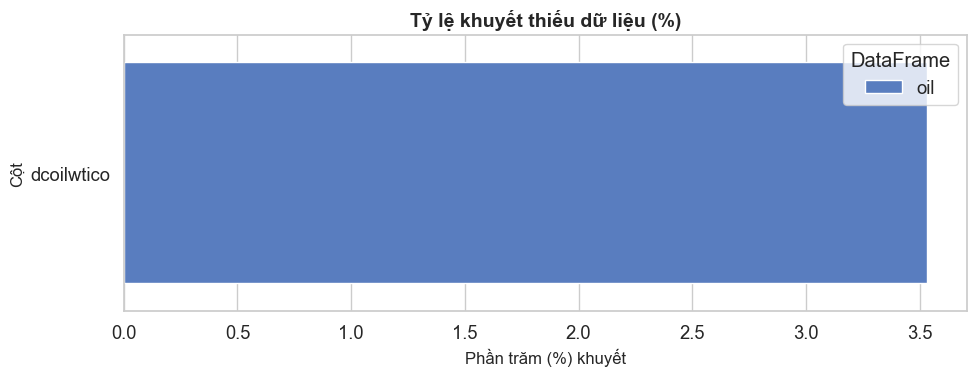
\includegraphics[width=0.78\textwidth]{figures/lab02/eda_001.png}
\caption{Missing values analysis — oil prices are missing on weekends/holidays due to market closure; all other columns are complete.}
\end{figure}

\subsubsection{2.2 — Target Distribution}
\texttt{sales} is heavily right-skewed (few high-sales days, many low-sales days). Three plots confirm:
\begin{itemize}
  \item Raw histogram: long right tail. \textbf{Decision:} train on $\log_{1p}(\text{sales})$ to approximate normality and stabilize variance.
  \item $\log_{1p}$ histogram: approximately normal — validates the training strategy.
  \item Boxplot: reveals outliers and the interquartile range. Zero sales > 10\% is normal (stores don't stock every family every day).
\end{itemize}

\begin{figure}[H]\centering
\begin{figure}[H]
  \centering
  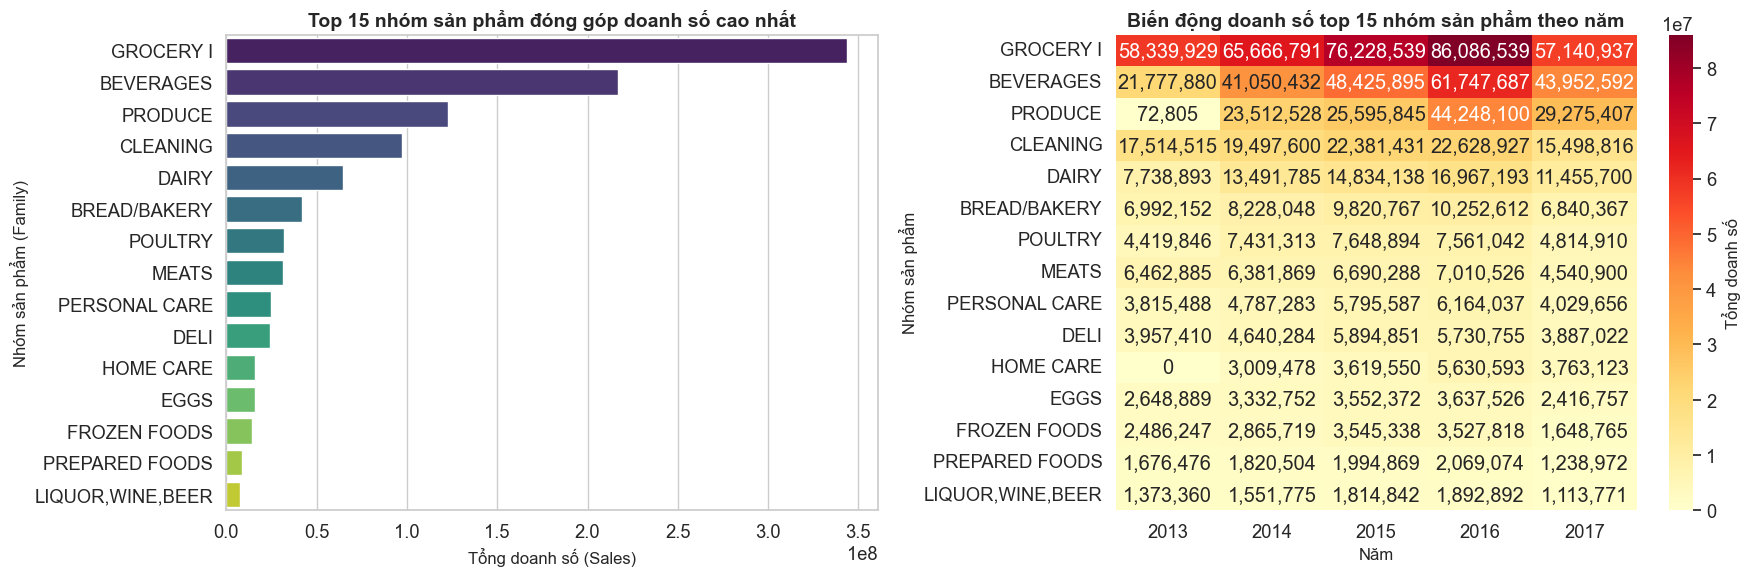
\includegraphics[width=\textwidth]{figures/lab02/eda_003.png}
  \caption{Target distribution — raw + $\log_{1p}$ — showing right skew.}
\end{figure}
\begin{figure}[H]
  \centering
  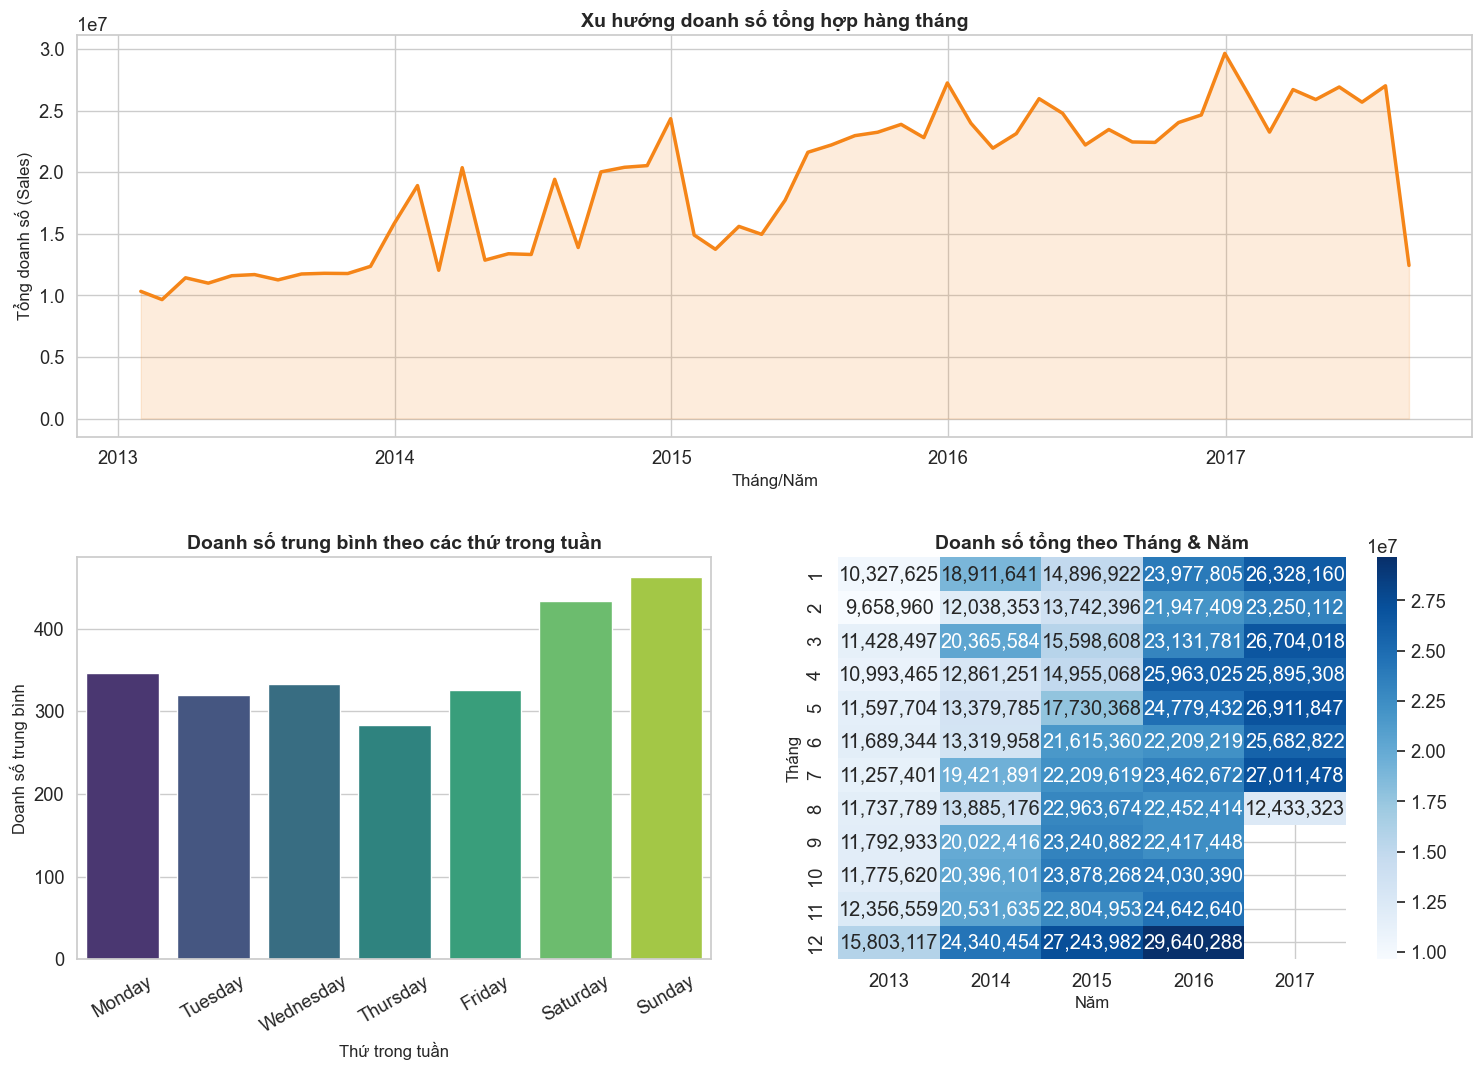
\includegraphics[width=0.7\textwidth]{figures/lab02/eda_004.png}
  \caption{Target boxplot by segments — reveals spread across different customer segments.}
\end{figure}
\begin{figure}[H]
  \centering
  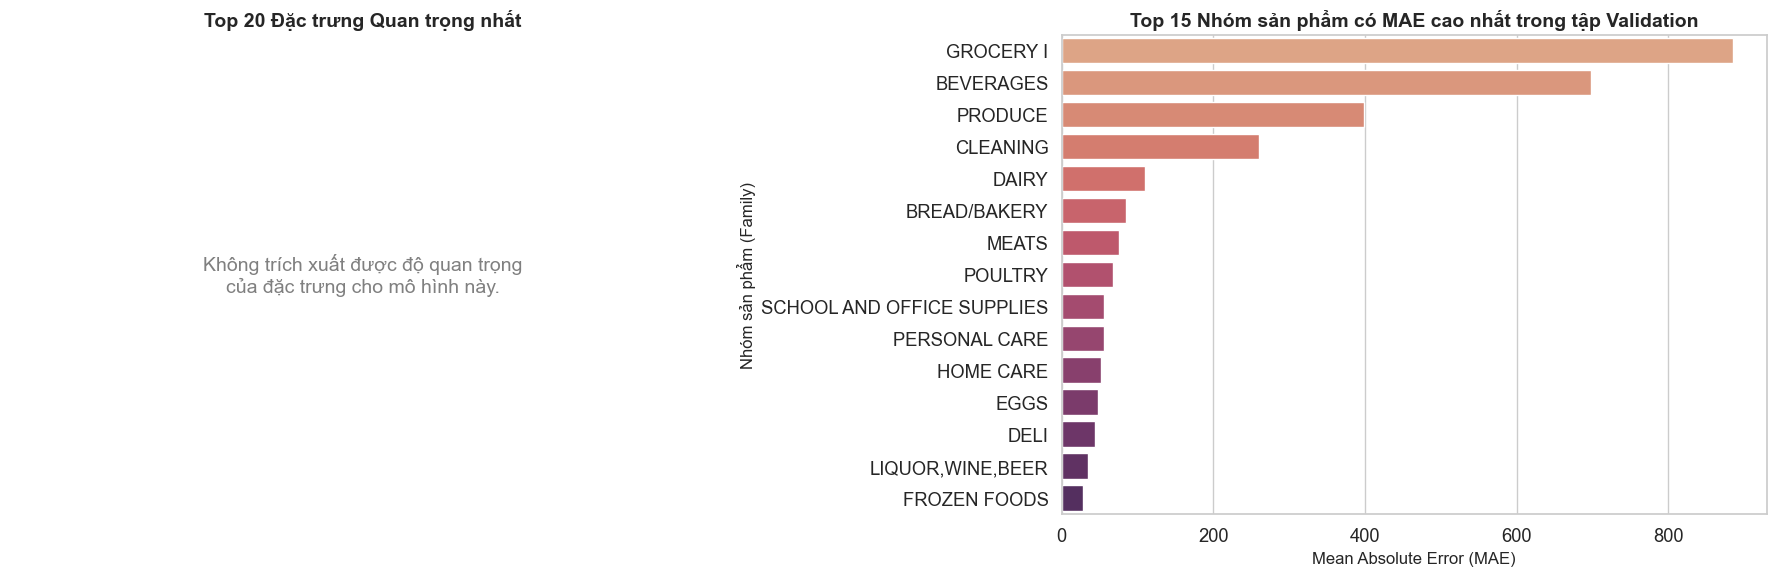
\includegraphics[width=0.7\textwidth]{figures/lab02/eda_018.png}
  \caption{Target distribution analysis: $\log_{1p}$ transform normalizes the heavily right-skewed sales data.}
\end{figure}
\end{figure}

\subsubsection{2.3 — Product Family Analysis}
Top-15 families by total sales show a Pareto distribution — \texttt{GROCERY I}, \texttt{BEVERAGES}, \texttt{PRODUCE} dominate revenue. Year-over-year heatmaps reveal whether market composition is shifting. This informs: should we train one global model or one per family?

\begin{figure}[H]\centering
\begin{figure}[H]
  \centering
  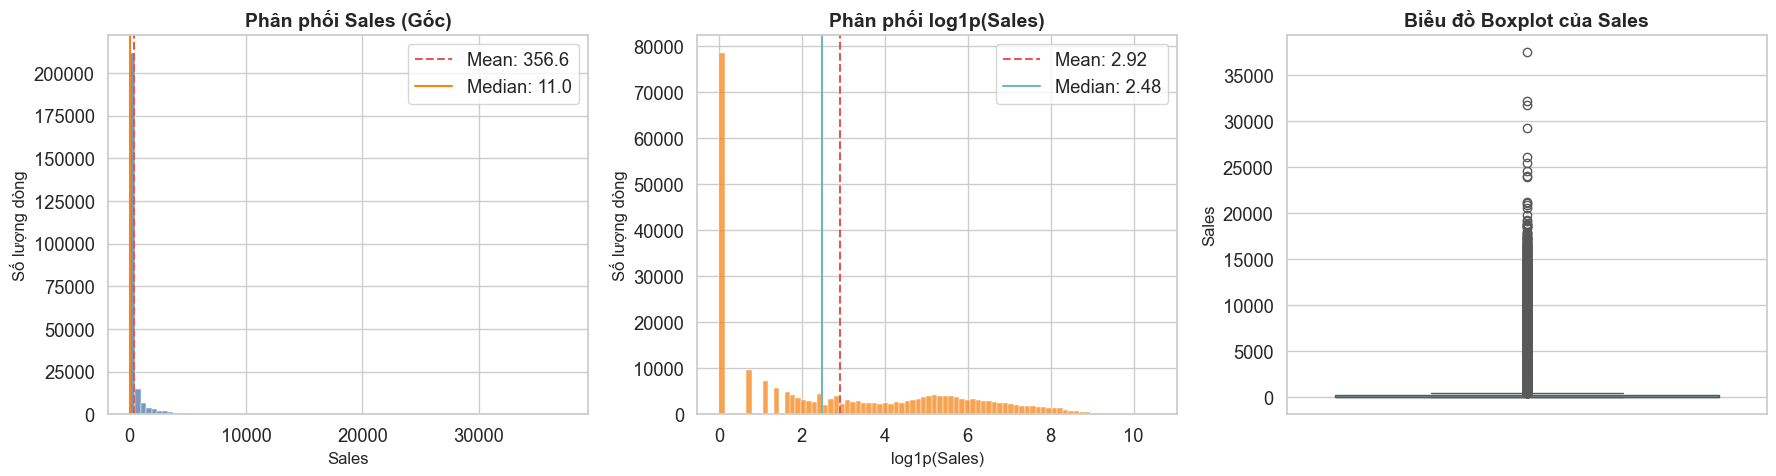
\includegraphics[width=\textwidth]{figures/lab02/eda_002.png}
  \caption{Product family revenue breakdown}
\end{figure}
\begin{figure}[H]
  \centering
  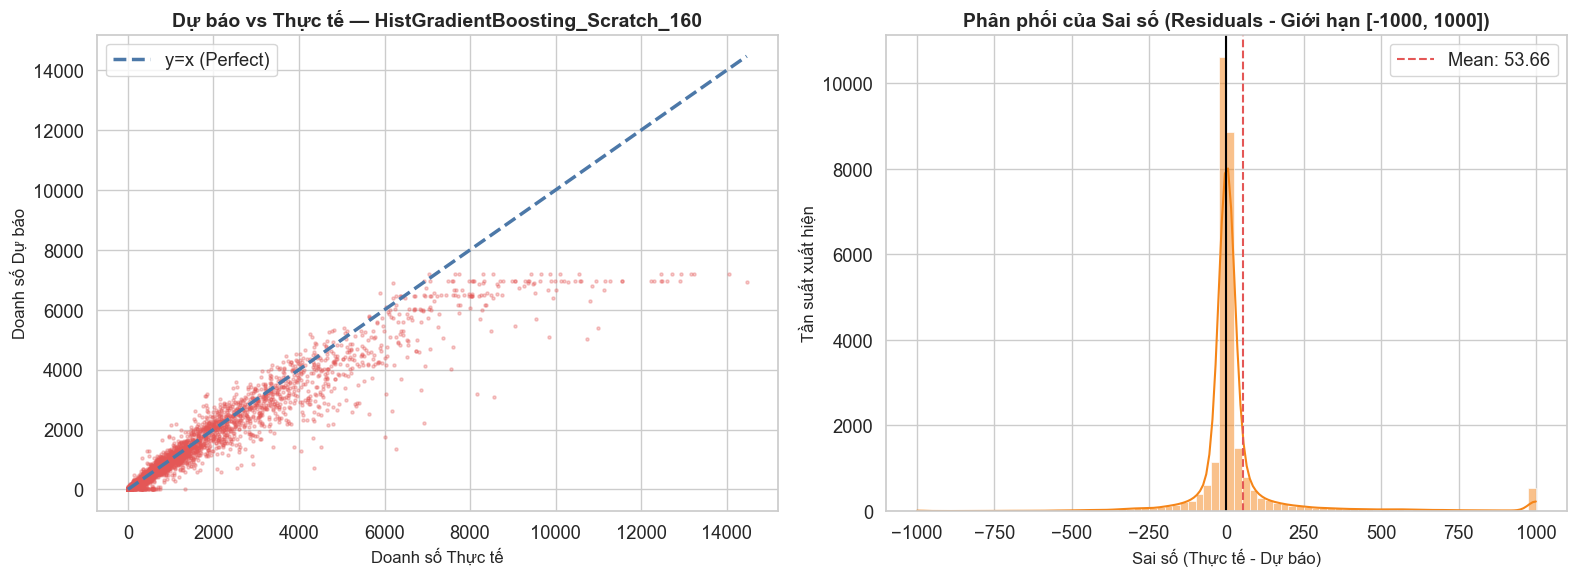
\includegraphics[width=\textwidth]{figures/lab02/eda_016.png}
  \caption{Revenue by category}
\end{figure}
\end{figure}

\subsubsection{2.4 — Trend and Seasonality}
Three plots reveal time-dependent patterns:
\begin{itemize}
  \item \textbf{Monthly total sales line chart:} Gradual growth trend over years.
  \item \textbf{Day-of-week bar chart:} Weekend sales > weekday sales — \texttt{is\_weekend} feature captures this.
  \item \textbf{Month $\times$ Year heatmap:} December spikes in holiday shopping season.
\end{itemize}

\begin{figure}[H]\centering
\begin{figure}[H]
  \centering
  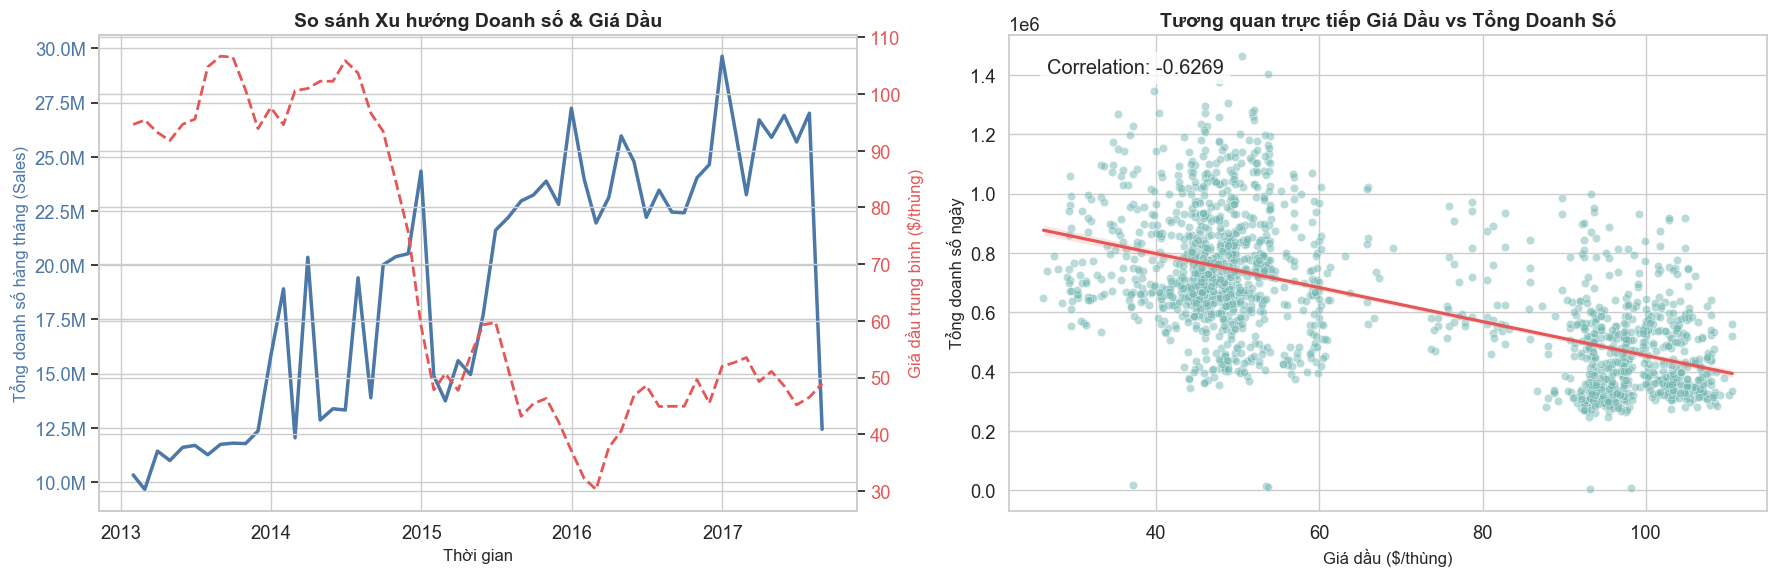
\includegraphics[width=\textwidth]{figures/lab02/eda_007.png}
  \caption{Daily revenue rolling mean — trend}
\end{figure}
\begin{figure}[H]
  \centering
  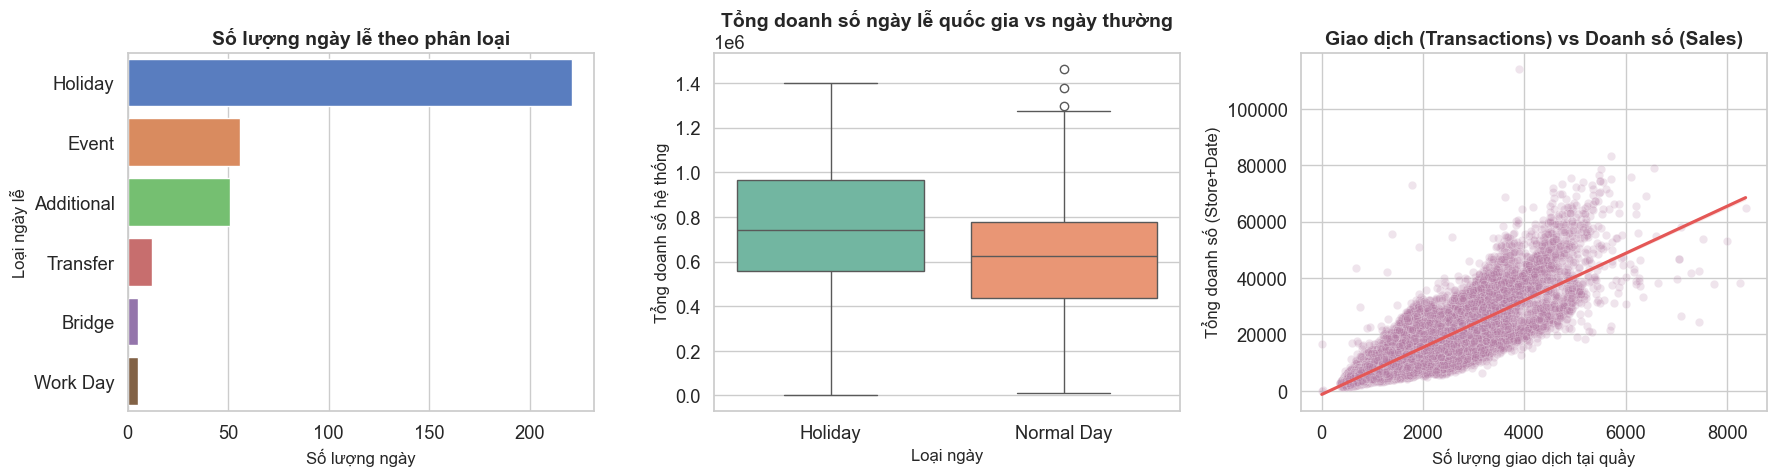
\includegraphics[width=\textwidth]{figures/lab02/eda_008.png}
  \caption{Monthly revenue patterns}
\end{figure}
\end{figure}

\subsubsection{2.5 — Promotion Impact}
\texttt{onpromotion} is bucketed (0, 1–5, 6–20, 20+) and correlated with sales. A scatter + regression line shows positive correlation, possibly with diminishing returns. Promotions are deployed more heavily around holidays — a potential confounder.

\begin{figure}[H]\centering
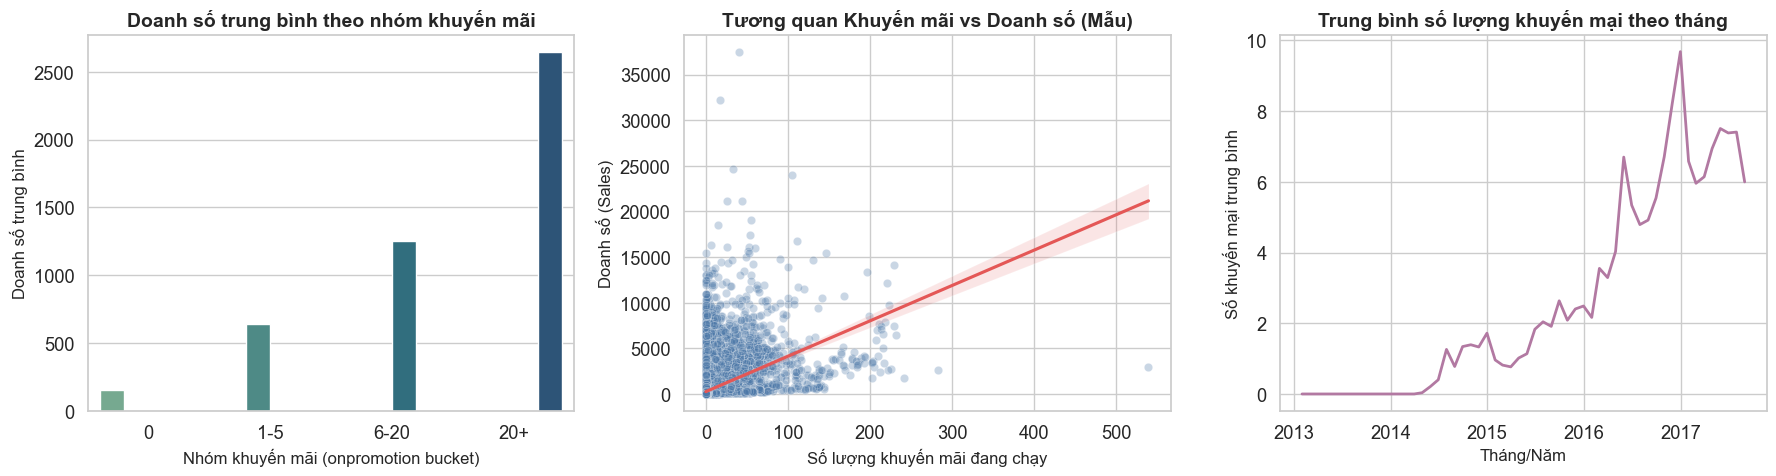
\includegraphics[width=0.78\textwidth]{figures/lab02/eda_005.png}
\caption{Promotion impact: \texttt{onpromotion} vs. sales showing positive correlation with diminishing returns at high promotion levels.}
\end{figure}

\subsubsection{2.6 — Store Characteristics}
Store \texttt{type} (A–E) reflects format/size; \texttt{cluster} reflects geographic/demographic grouping. Boxplots reveal: Type A stores have the highest volume; even within the same type, variance is large (location matters). If type/cluster explains >20\% of sales variance, these features are essential.

\begin{figure}[H]\centering
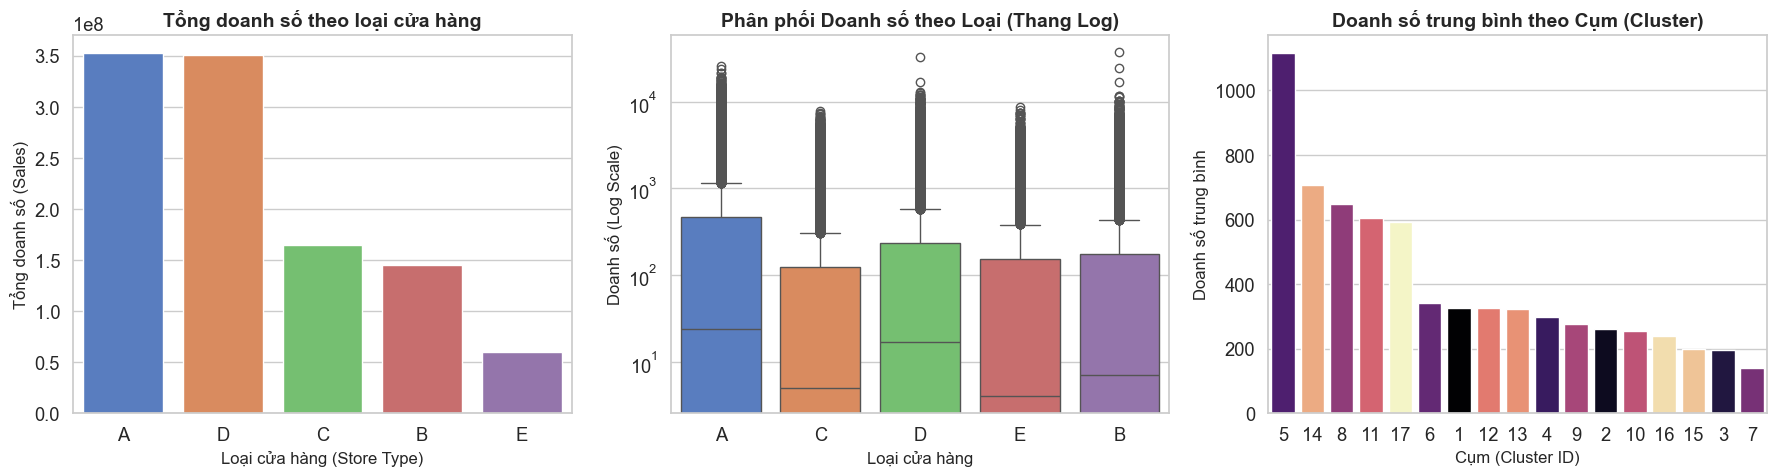
\includegraphics[width=0.78\textwidth]{figures/lab02/eda_006.png}
\caption{Store characteristics: sales distribution by store type and cluster. Type A dominates volume; intra-type variance signals local effects.}
\end{figure}

\subsubsection{2.7 — Oil Price Correlation}
Ecuador is a major oil exporter — oil prices affect consumer spending. A dual-axis plot overlays monthly sales with average oil price; a scatter + regression shows correlation. Mild positive correlation (0.2–0.4) expected — oil changes slowly, helping detect macro-economic shifts that pure sales history misses.

\subsubsection{2.8 — Holidays and Transactions}
\texttt{transactions} (store traffic) correlates strongly with sales ($r > 0.8$). However, \texttt{transactions} is unavailable in \texttt{test.csv} — it is an \textbf{EDA reference variable only}, not a model feature. National holidays show higher sales than normal days; \texttt{transferred=True} holidays are excluded (Ecuador moves holidays to Monday, making the original date a regular workday).

\begin{figure}[H]\centering
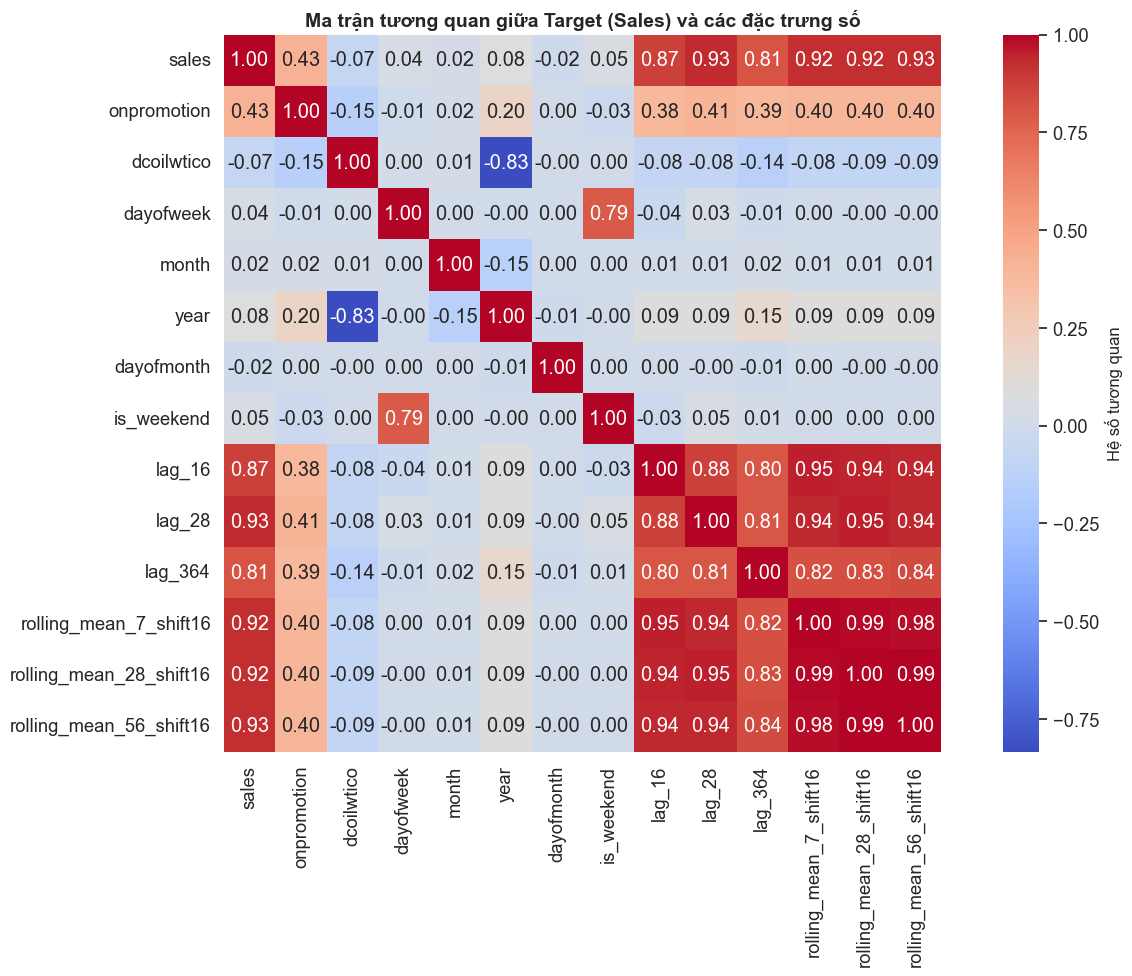
\includegraphics[width=0.78\textwidth]{figures/lab02/eda_009.png}
\caption{Holiday analysis: sales patterns around national holidays — higher sales on holiday dates vs. normal days.}
\end{figure}

\begin{figure}[H]\centering
\begin{figure}[H]
  \centering
  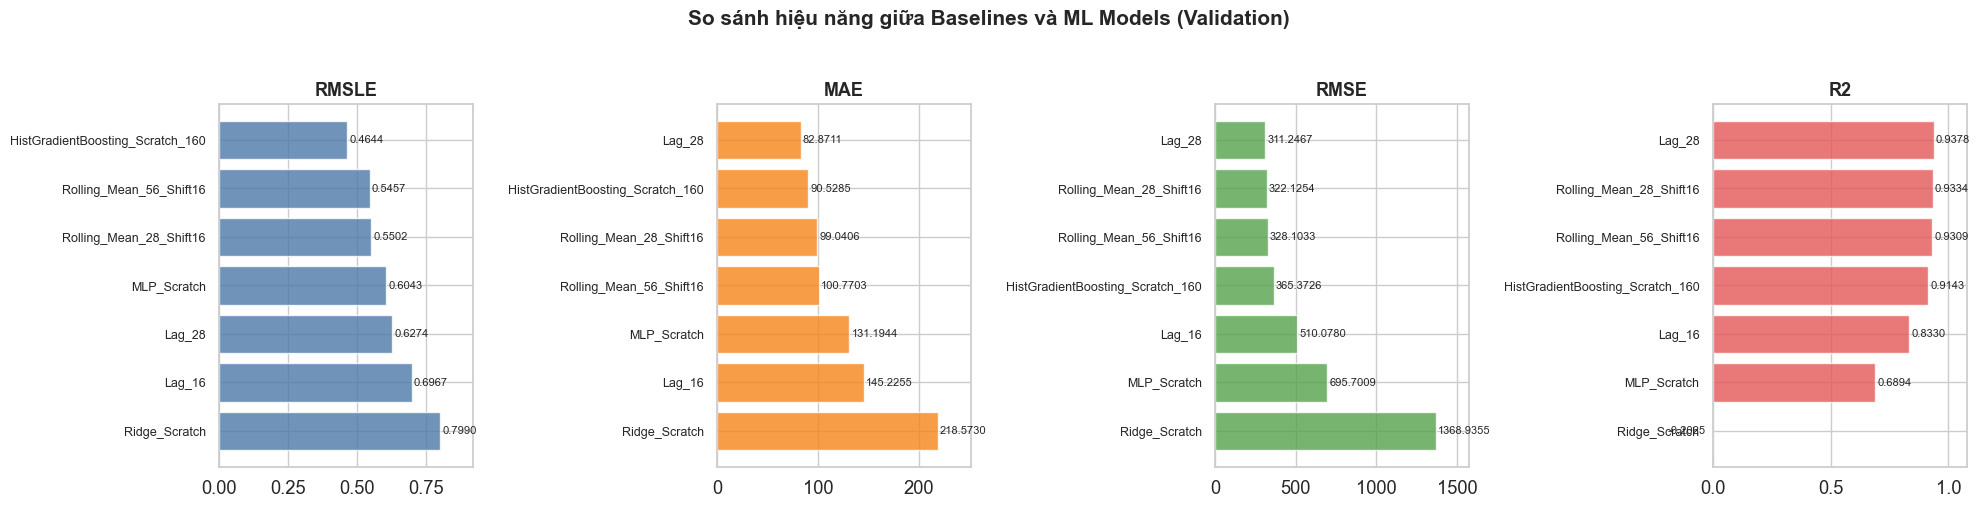
\includegraphics[width=\textwidth]{figures/lab02/eda_010.png}
  \caption{Revenue distribution}
\end{figure}
\begin{figure}[H]
  \centering
  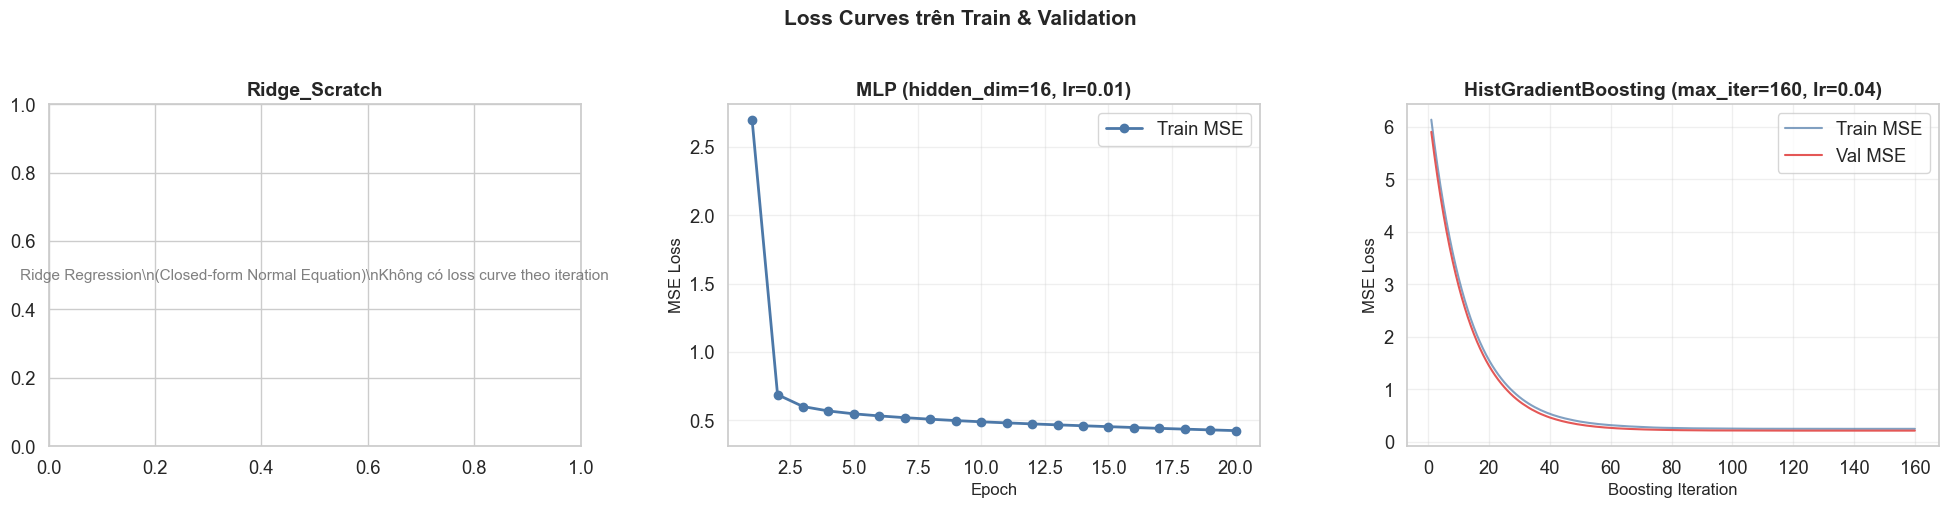
\includegraphics[width=\textwidth]{figures/lab02/eda_011.png}
  \caption{Revenue boxplot by store}
\end{figure}\
\vspace{4pt}
\begin{figure}[H]
  \centering
  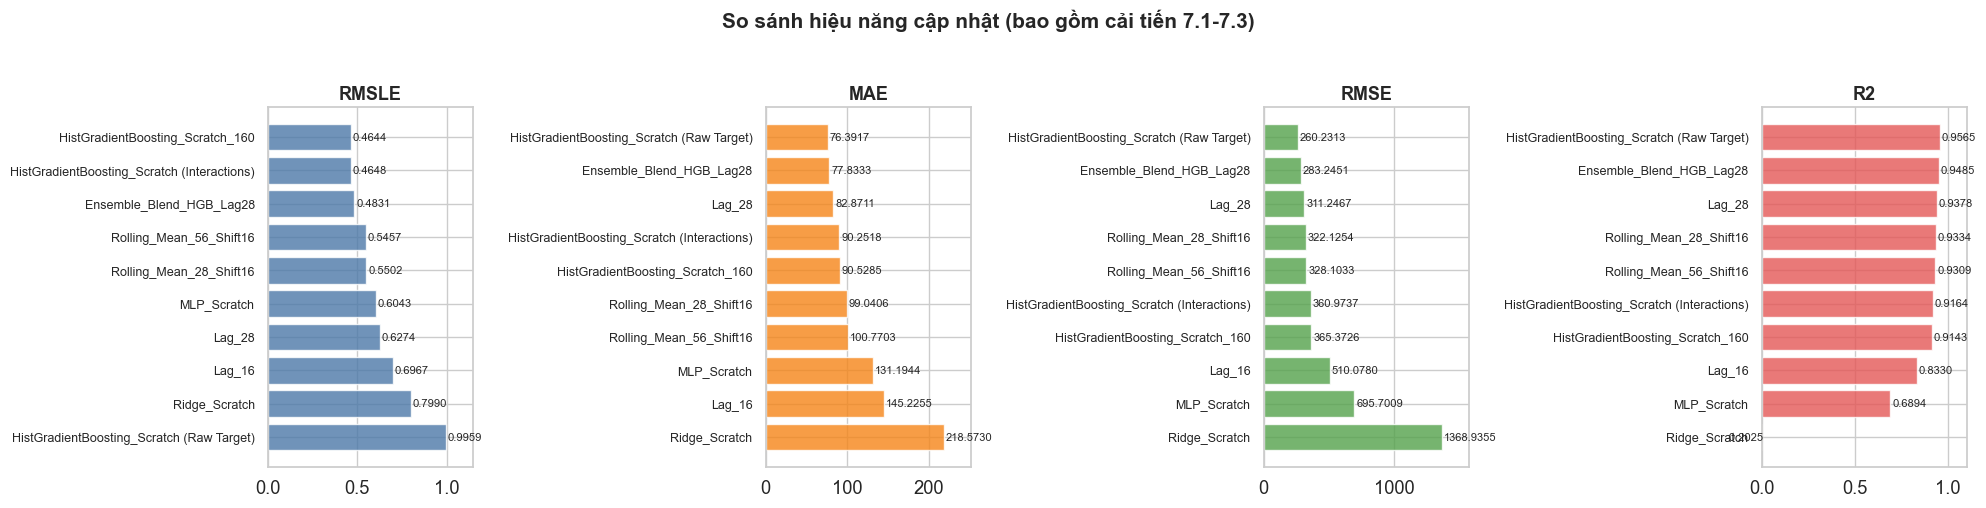
\includegraphics[width=\textwidth]{figures/lab02/eda_012.png}
  \caption{Quantity vs. revenue}
\end{figure}
\begin{figure}[H]
  \centering
  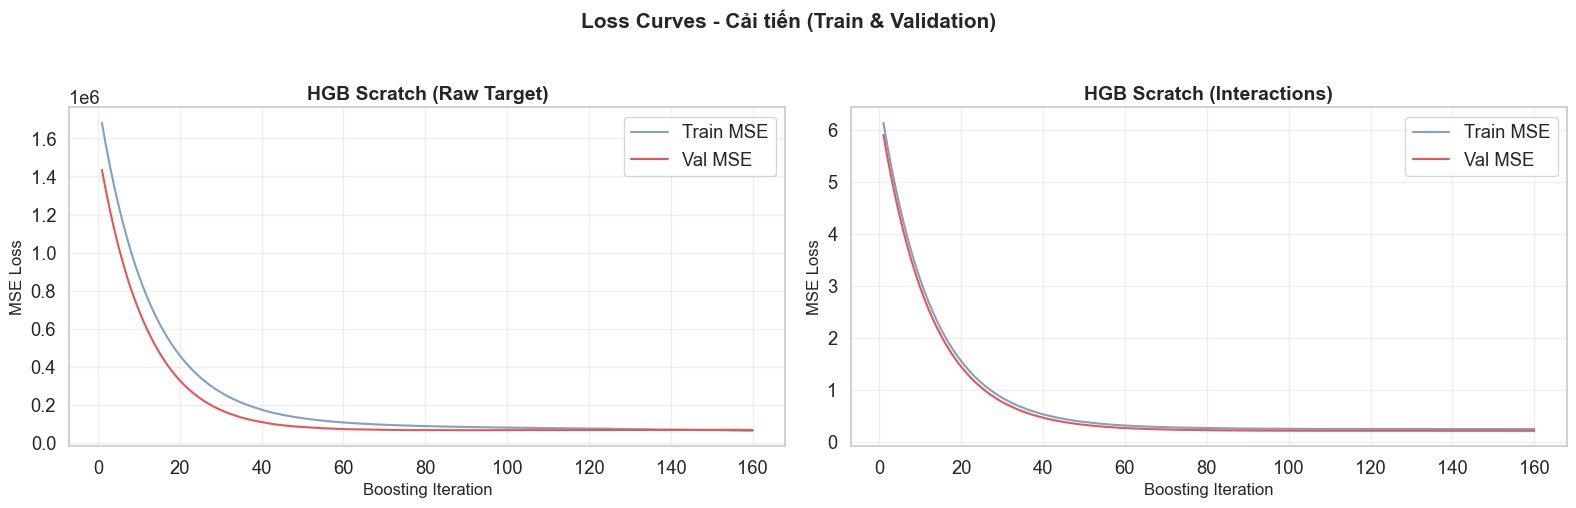
\includegraphics[width=\textwidth]{figures/lab02/eda_013.png}
  \caption{Unit price vs. revenue}
\end{figure}
\end{figure}

\begin{figure}[H]\centering
\begin{figure}[H]
  \centering
  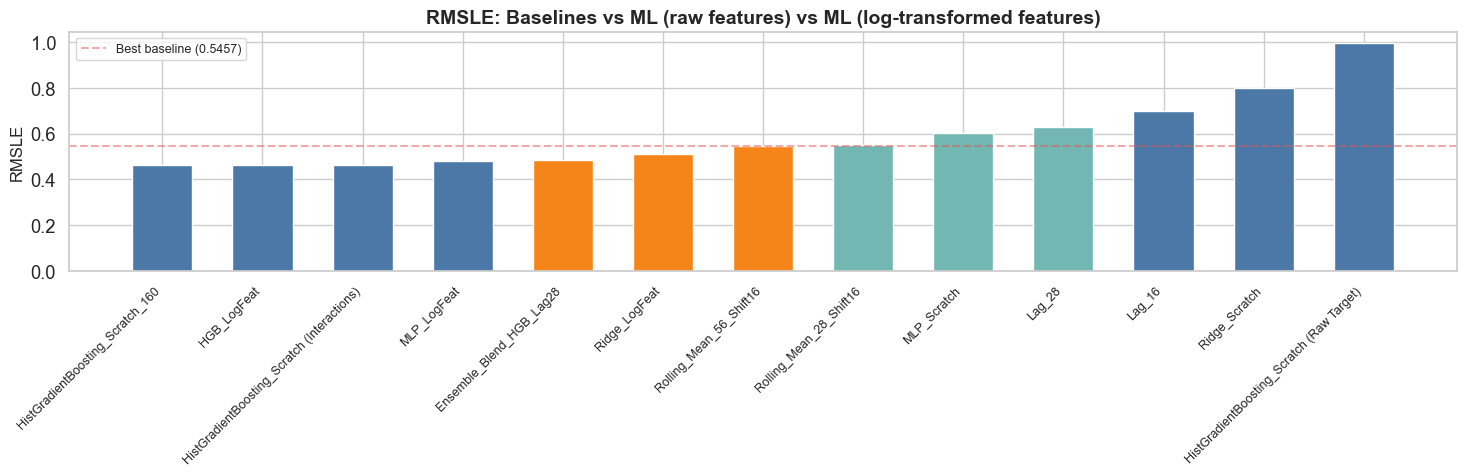
\includegraphics[width=\textwidth]{figures/lab02/eda_014.png}
  \caption{Revenue by region}
\end{figure}
\begin{figure}[H]
  \centering
  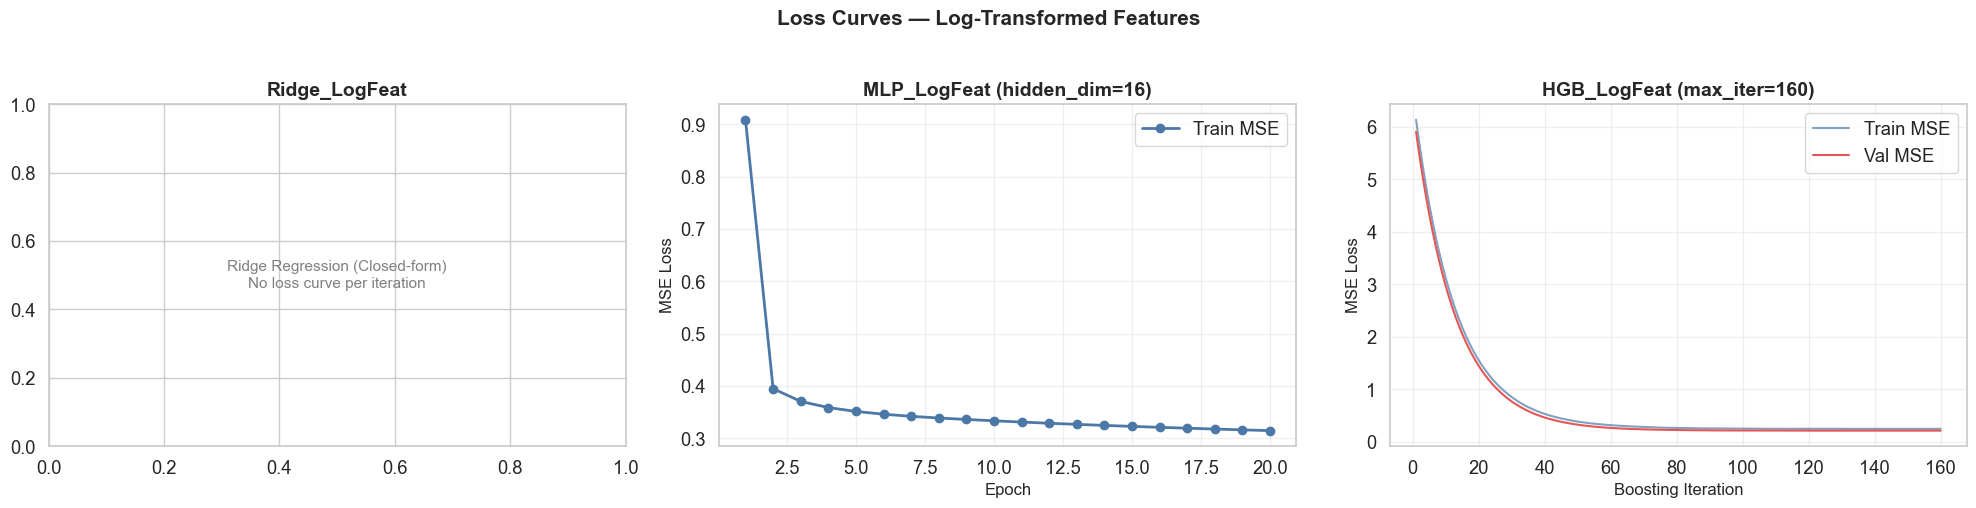
\includegraphics[width=\textwidth]{figures/lab02/eda_015.png}
  \caption{Top states by revenue}
\end{figure}\
\vspace{4pt}
\begin{figure}[H]
  \centering
  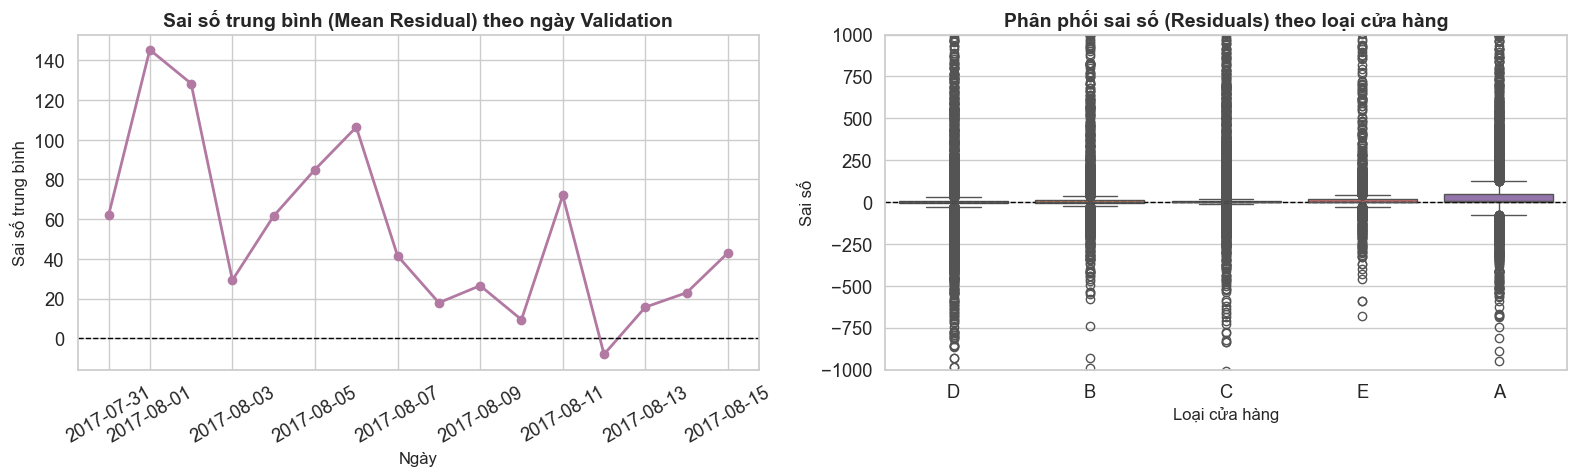
\includegraphics[width=\textwidth]{figures/lab02/eda_017.png}
  \caption{Top products by revenue}
\end{figure}
\begin{figure}[H]
  \centering
  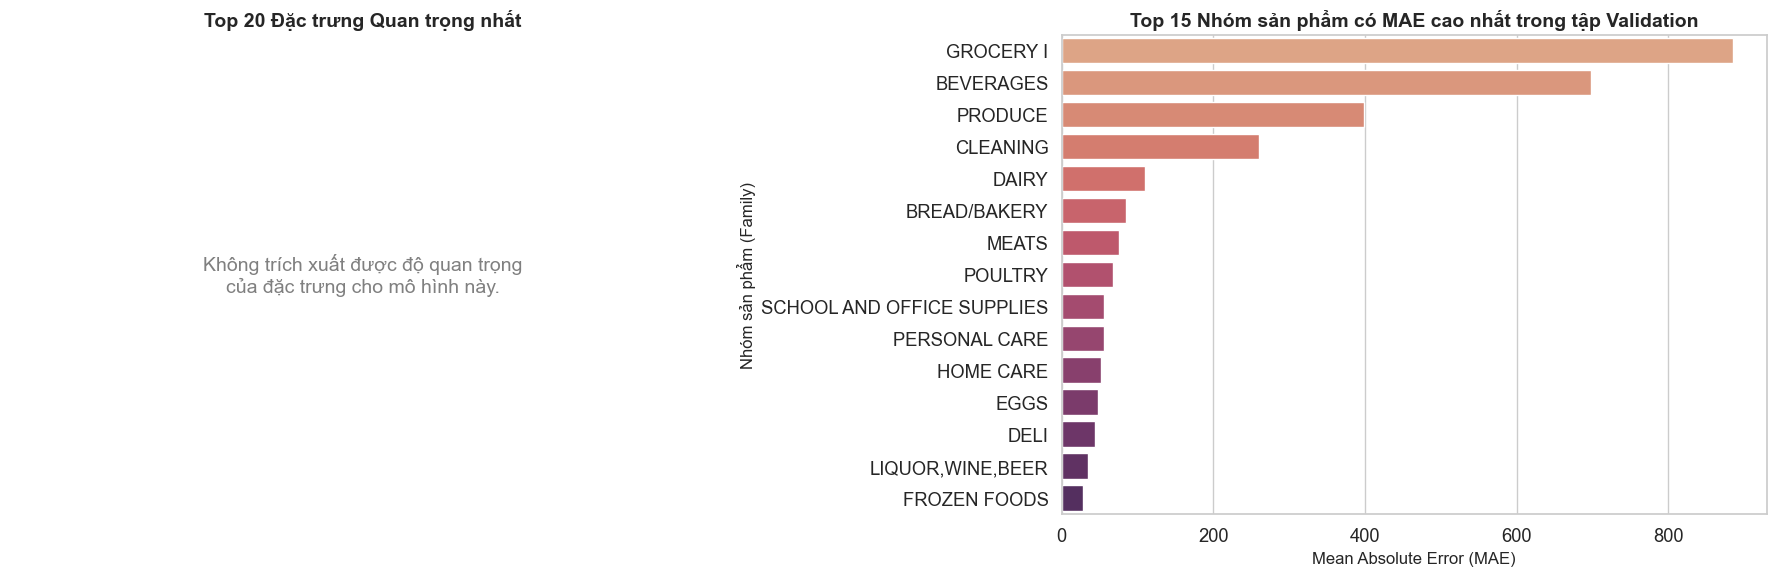
\includegraphics[width=\textwidth]{figures/lab02/eda_018.png}
  \caption{Revenue by category detail}
\end{figure}
\end{figure}

\begin{figure}[H]\centering
\begin{figure}[H]
  \centering
  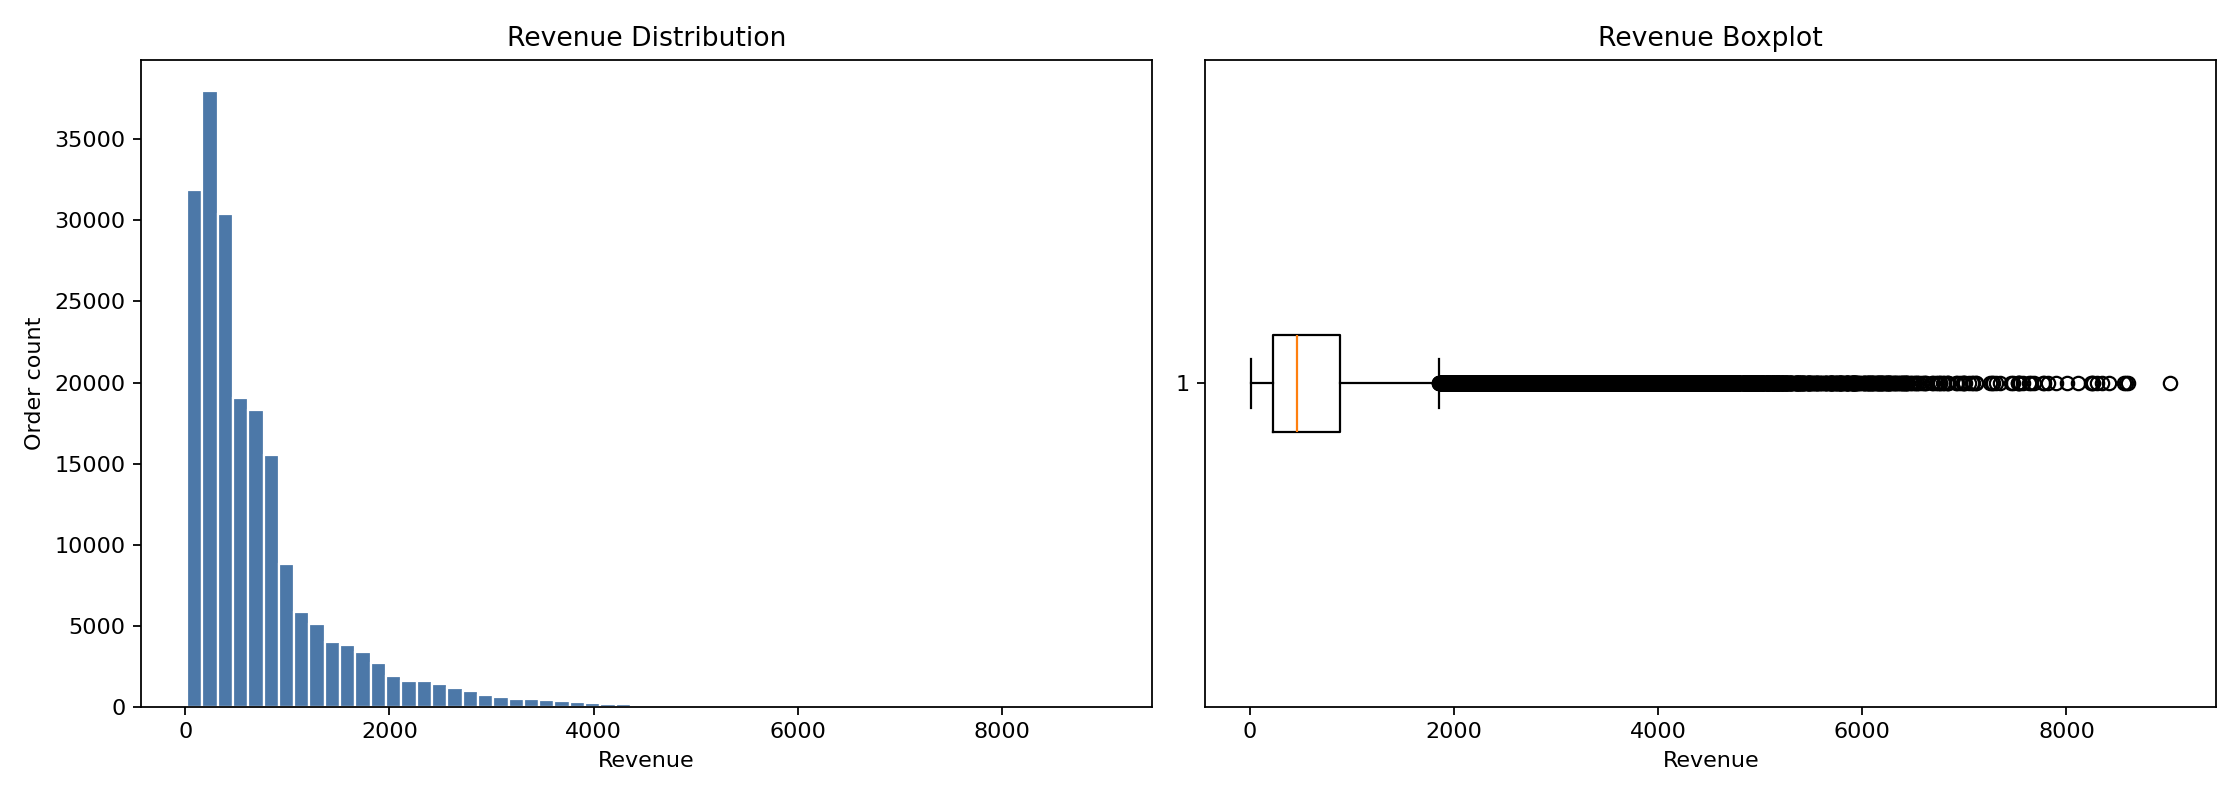
\includegraphics[width=\textwidth]{figures/lab02/notebook_revenue_distribution_boxplot.png}
  \caption{Revenue distribution boxplot}
\end{figure}
\begin{figure}[H]
  \centering
  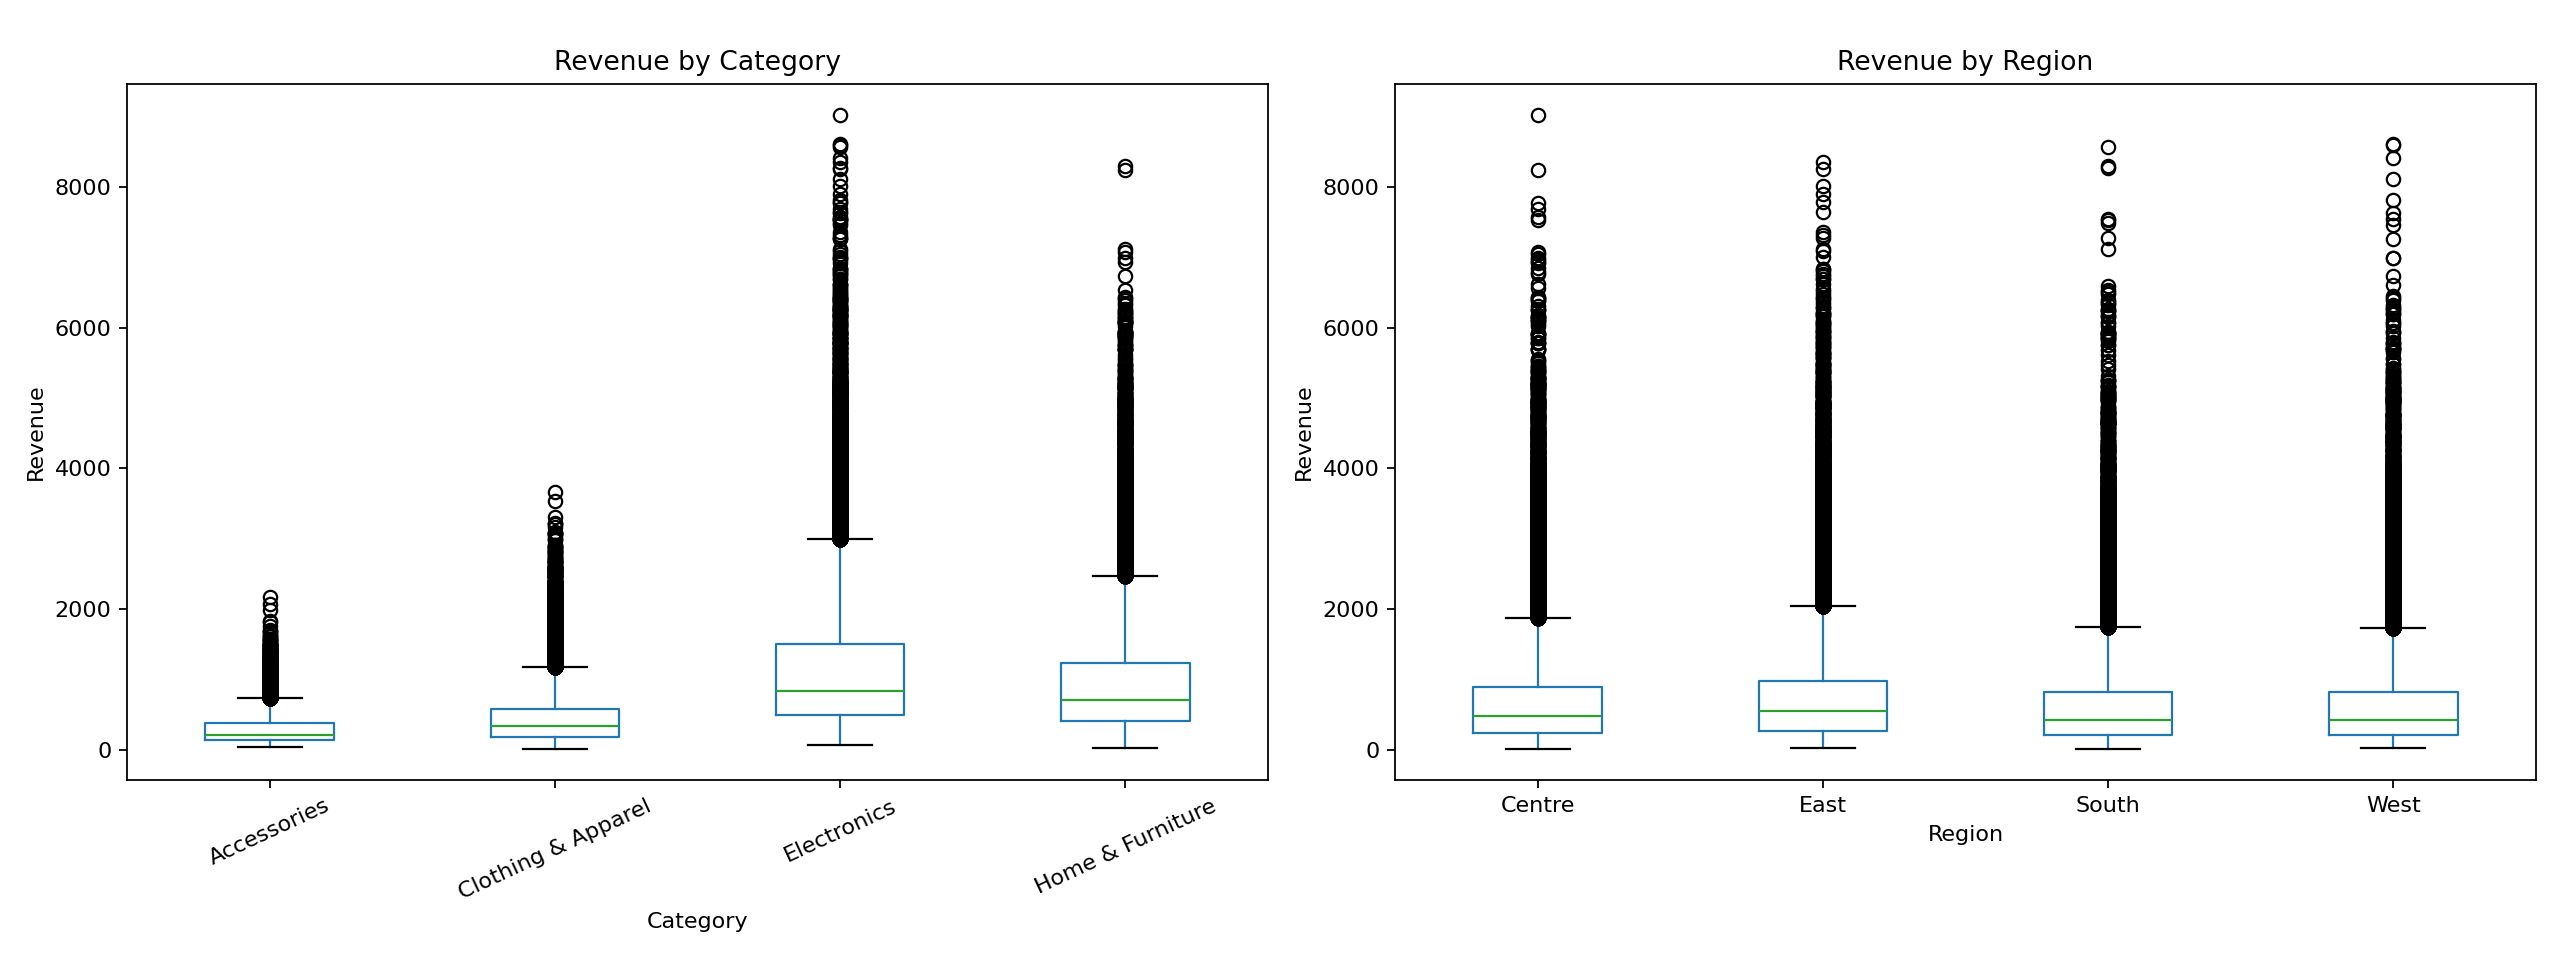
\includegraphics[width=\textwidth]{figures/lab02/notebook_revenue_boxplot_by_segments.png}
  \caption{Revenue by segments}
\end{figure}\
\vspace{4pt}
\begin{figure}[H]
  \centering
  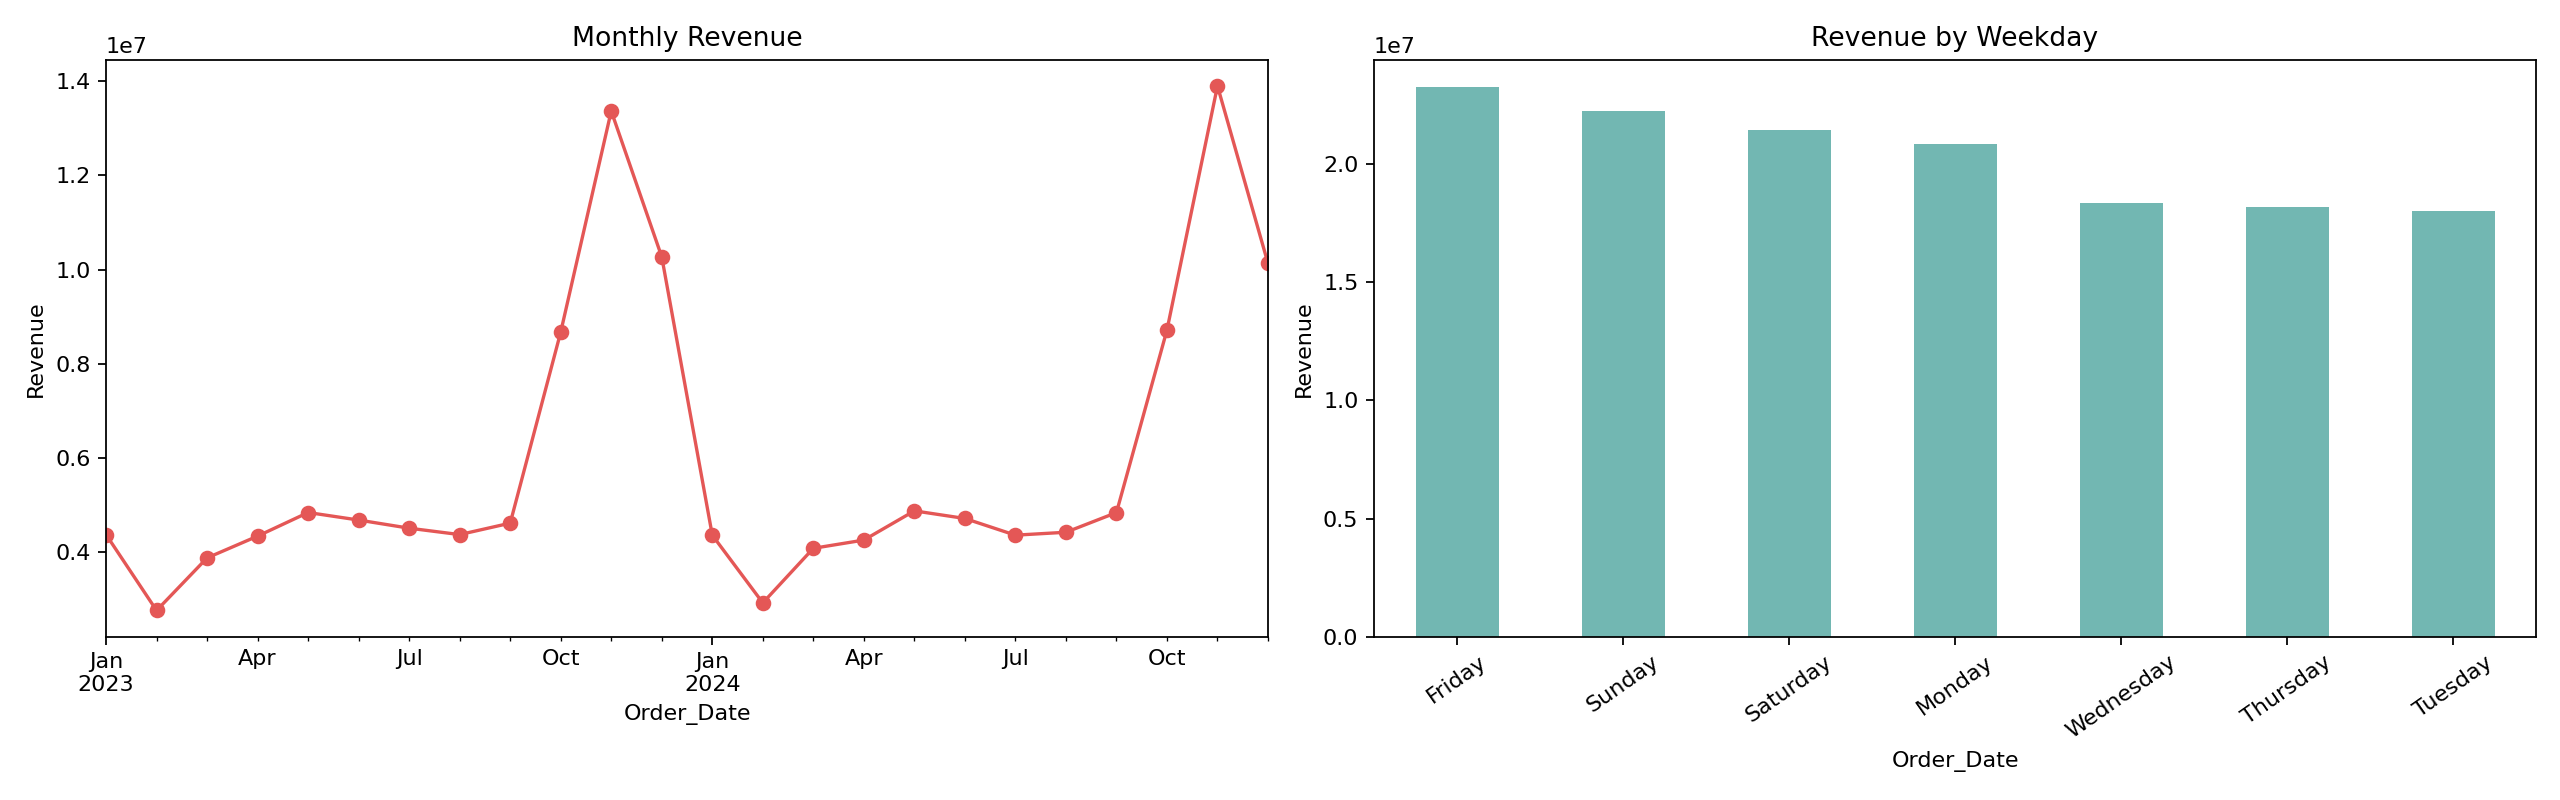
\includegraphics[width=\textwidth]{figures/lab02/notebook_time_eda.png}
  \caption{Time-series EDA patterns}
\end{figure}
\begin{figure}[H]
  \centering
  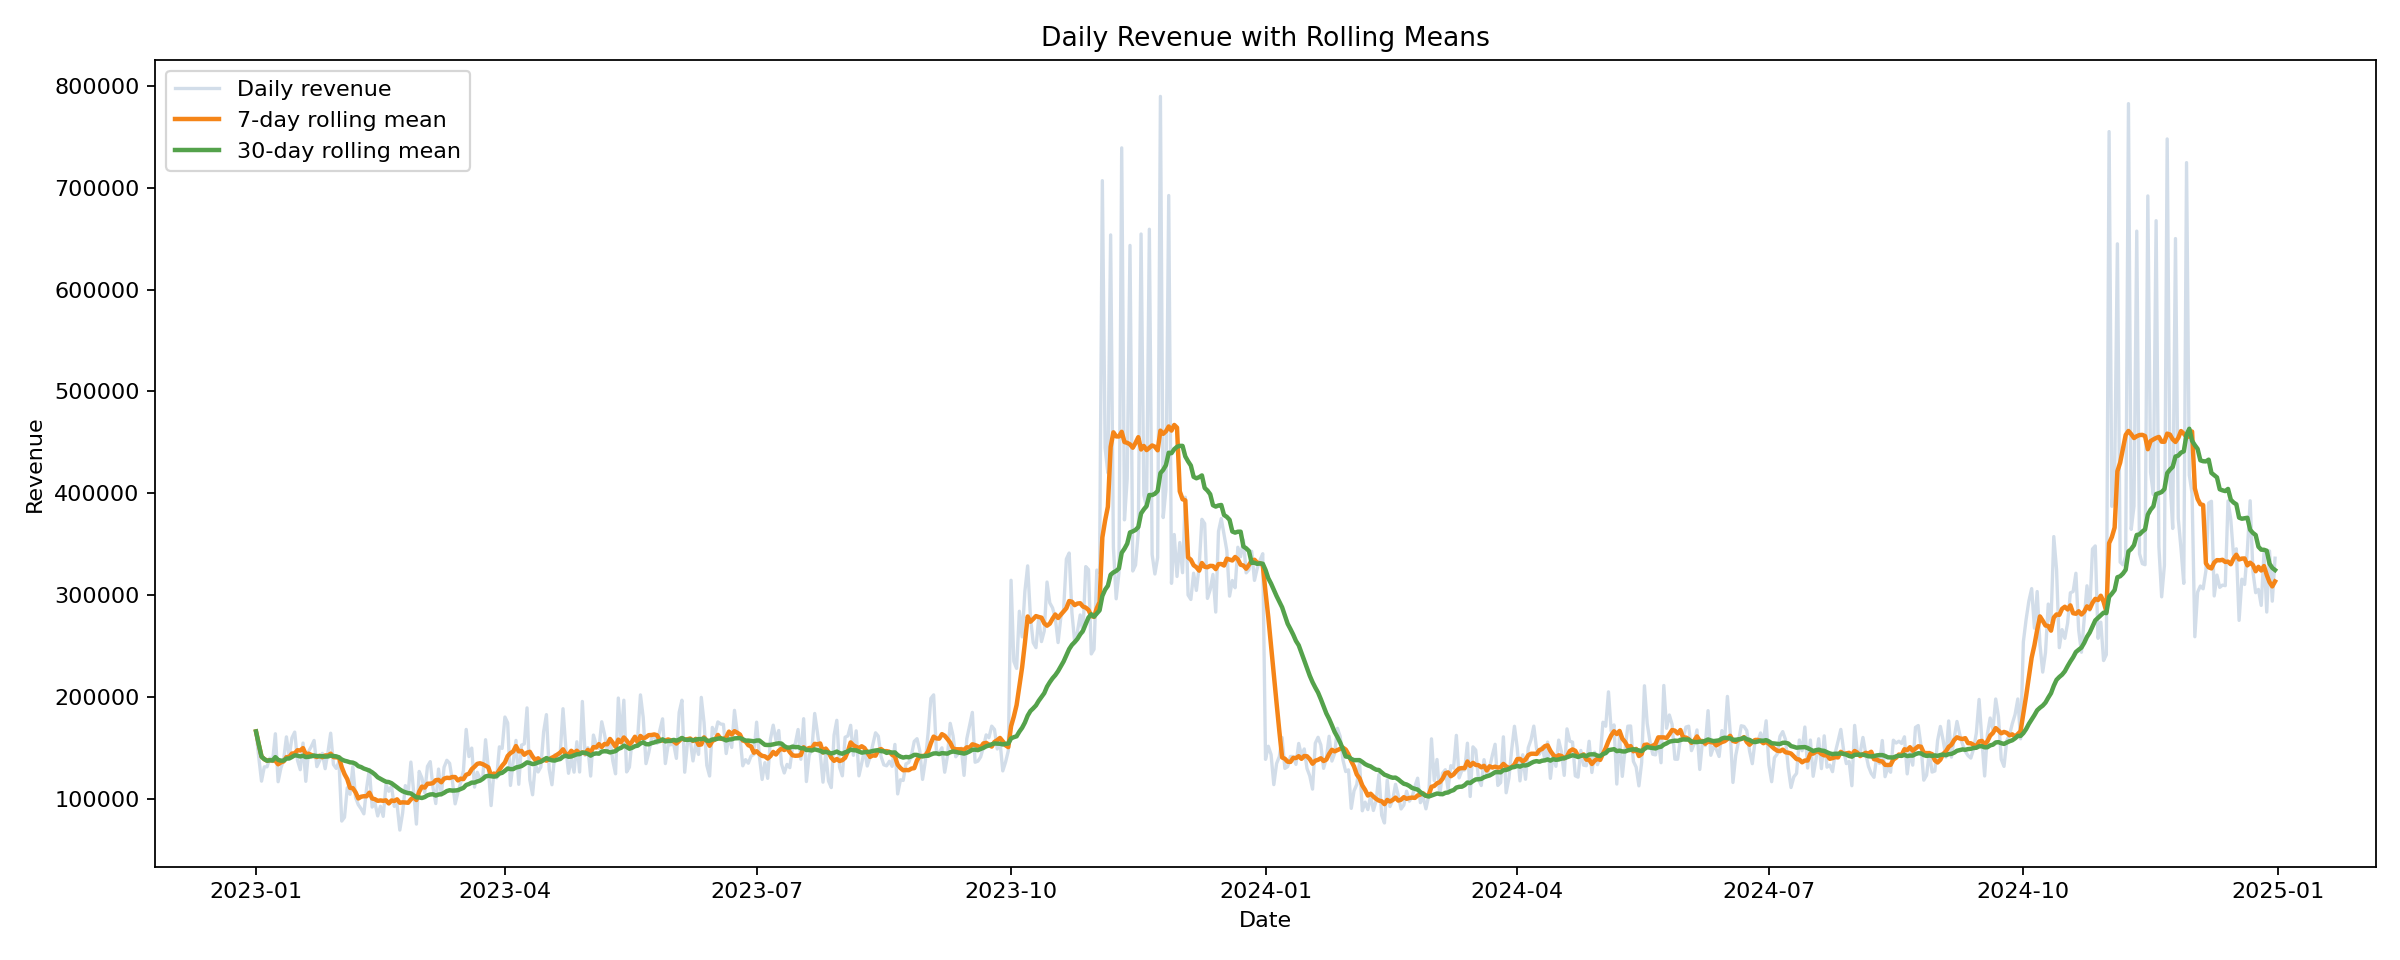
\includegraphics[width=\textwidth]{figures/lab02/notebook_daily_revenue_rolling_mean.png}
  \caption{Daily revenue rolling mean}
\end{figure}
\end{figure}

\begin{figure}[H]\centering
\begin{figure}[H]
  \centering
  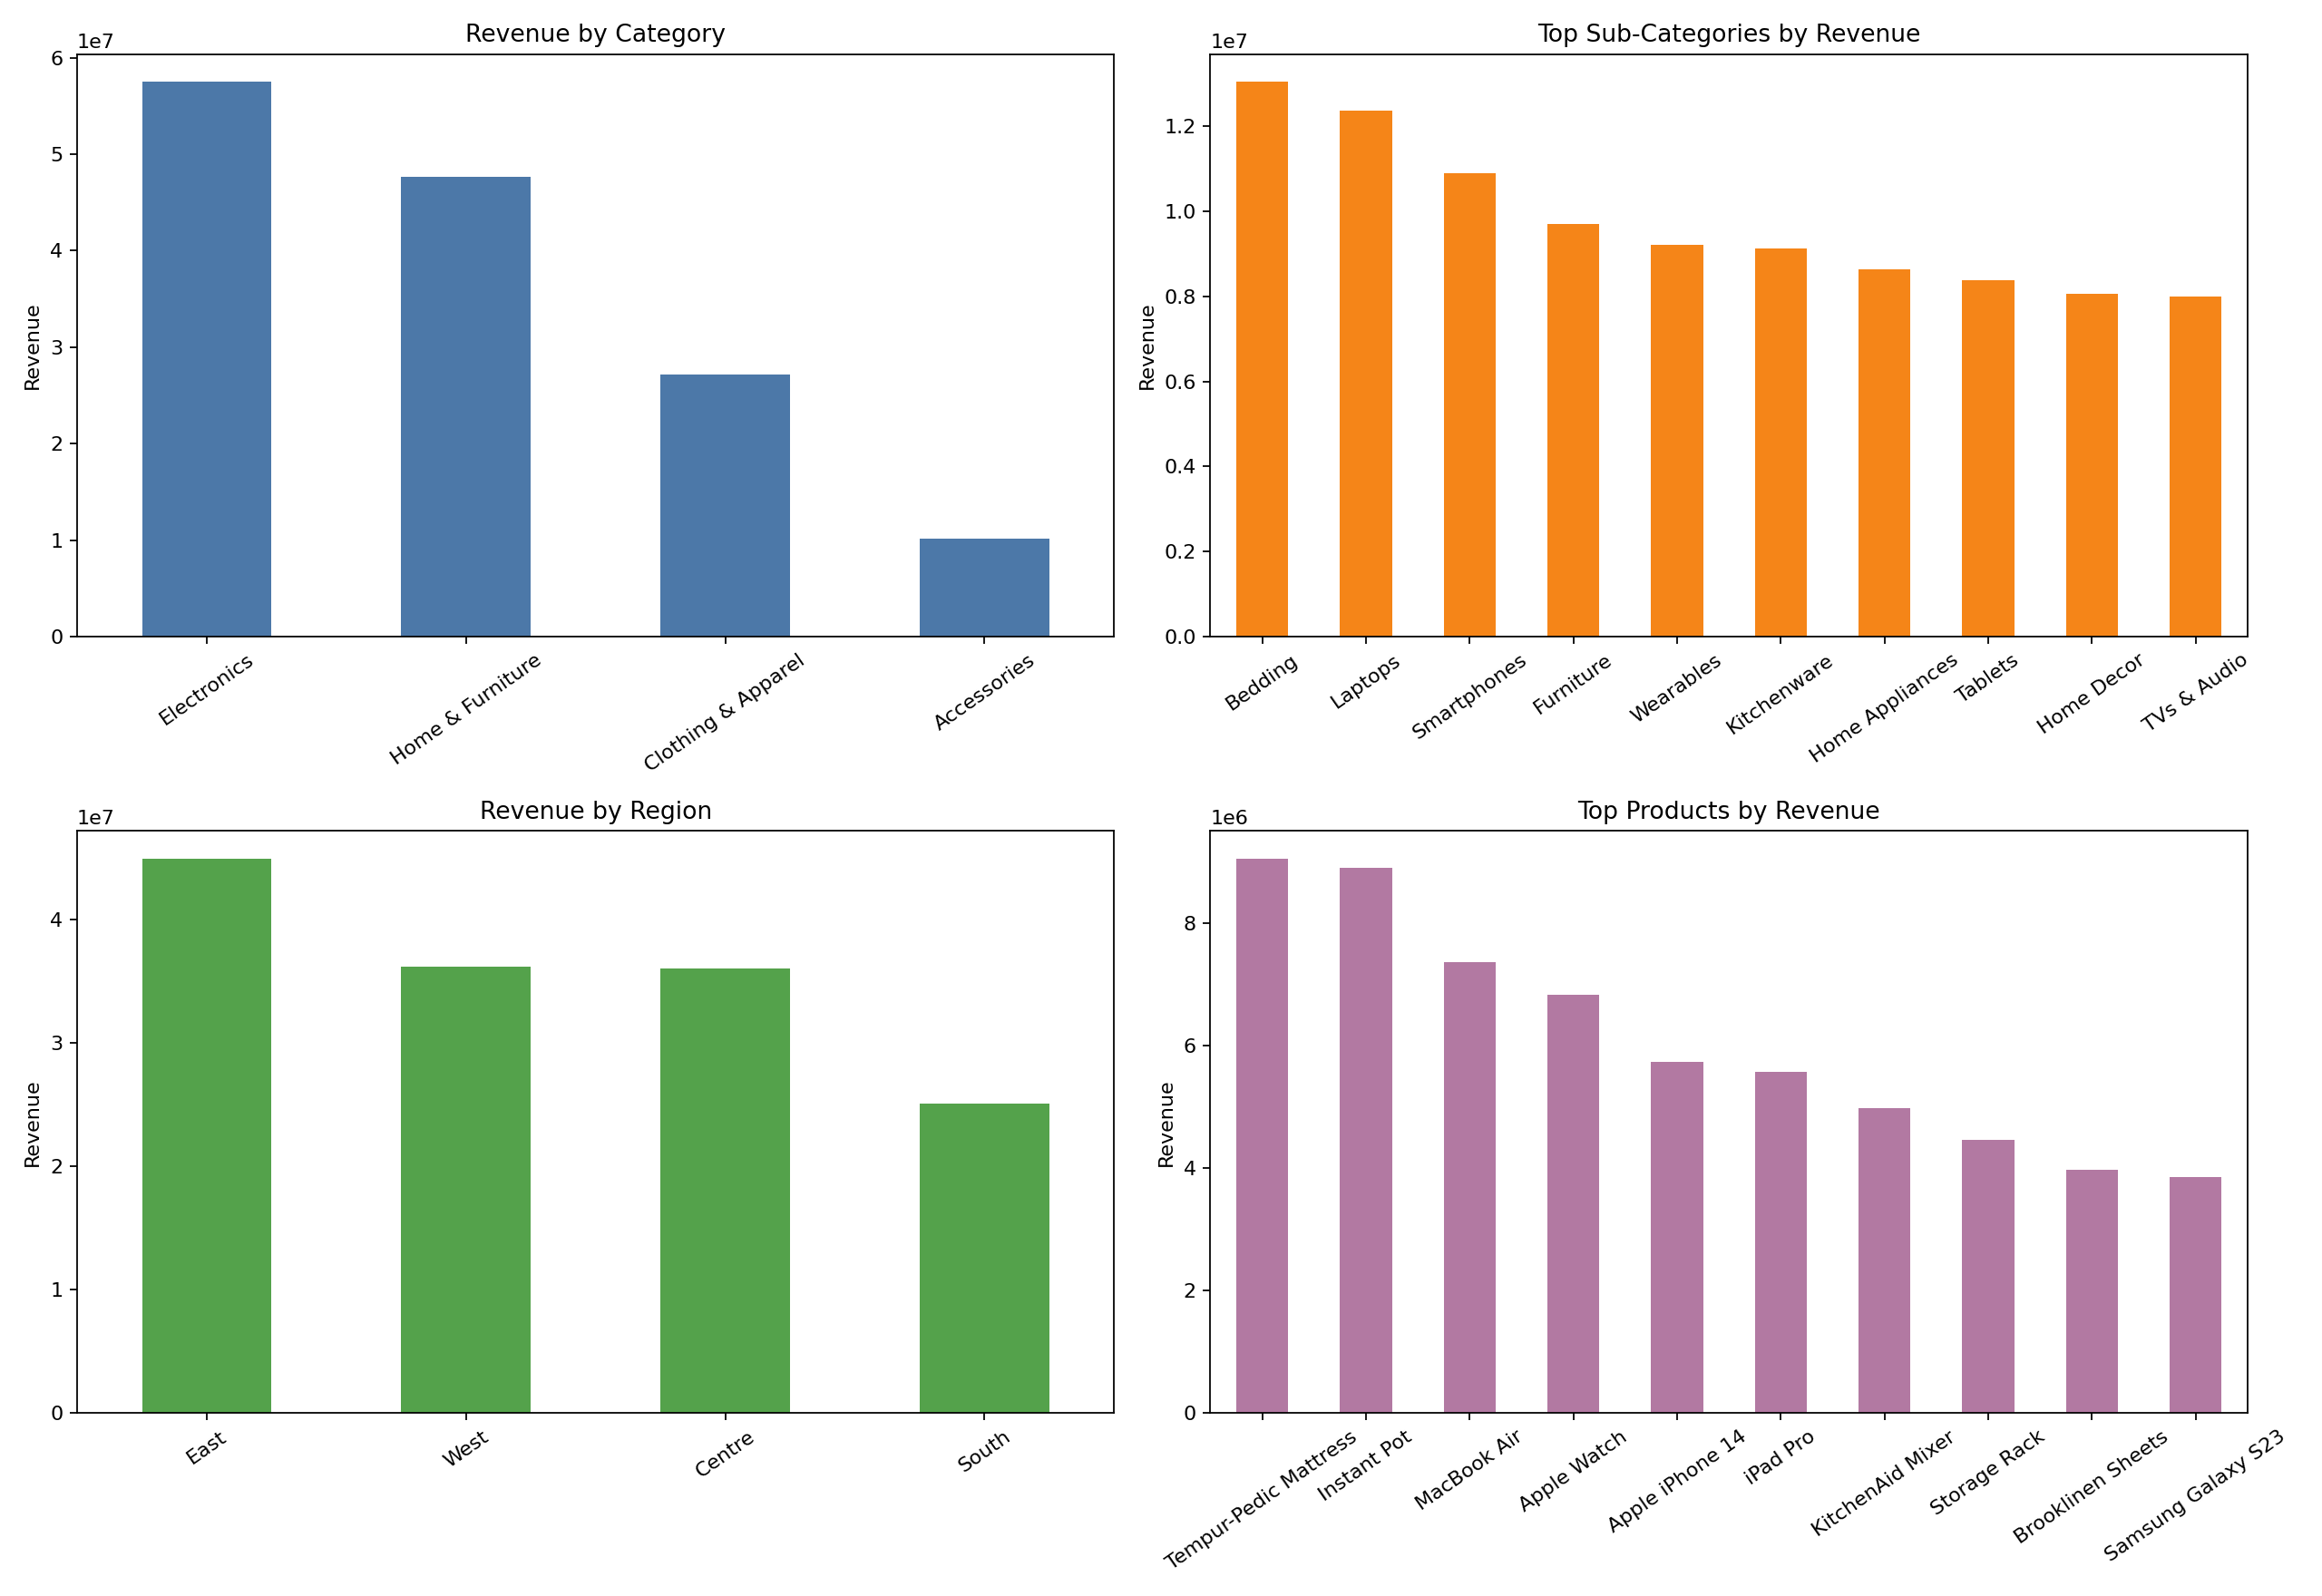
\includegraphics[width=\textwidth]{figures/lab02/notebook_product_geography_eda.png}
  \caption{Product geography analysis}
\end{figure}
\begin{figure}[H]
  \centering
  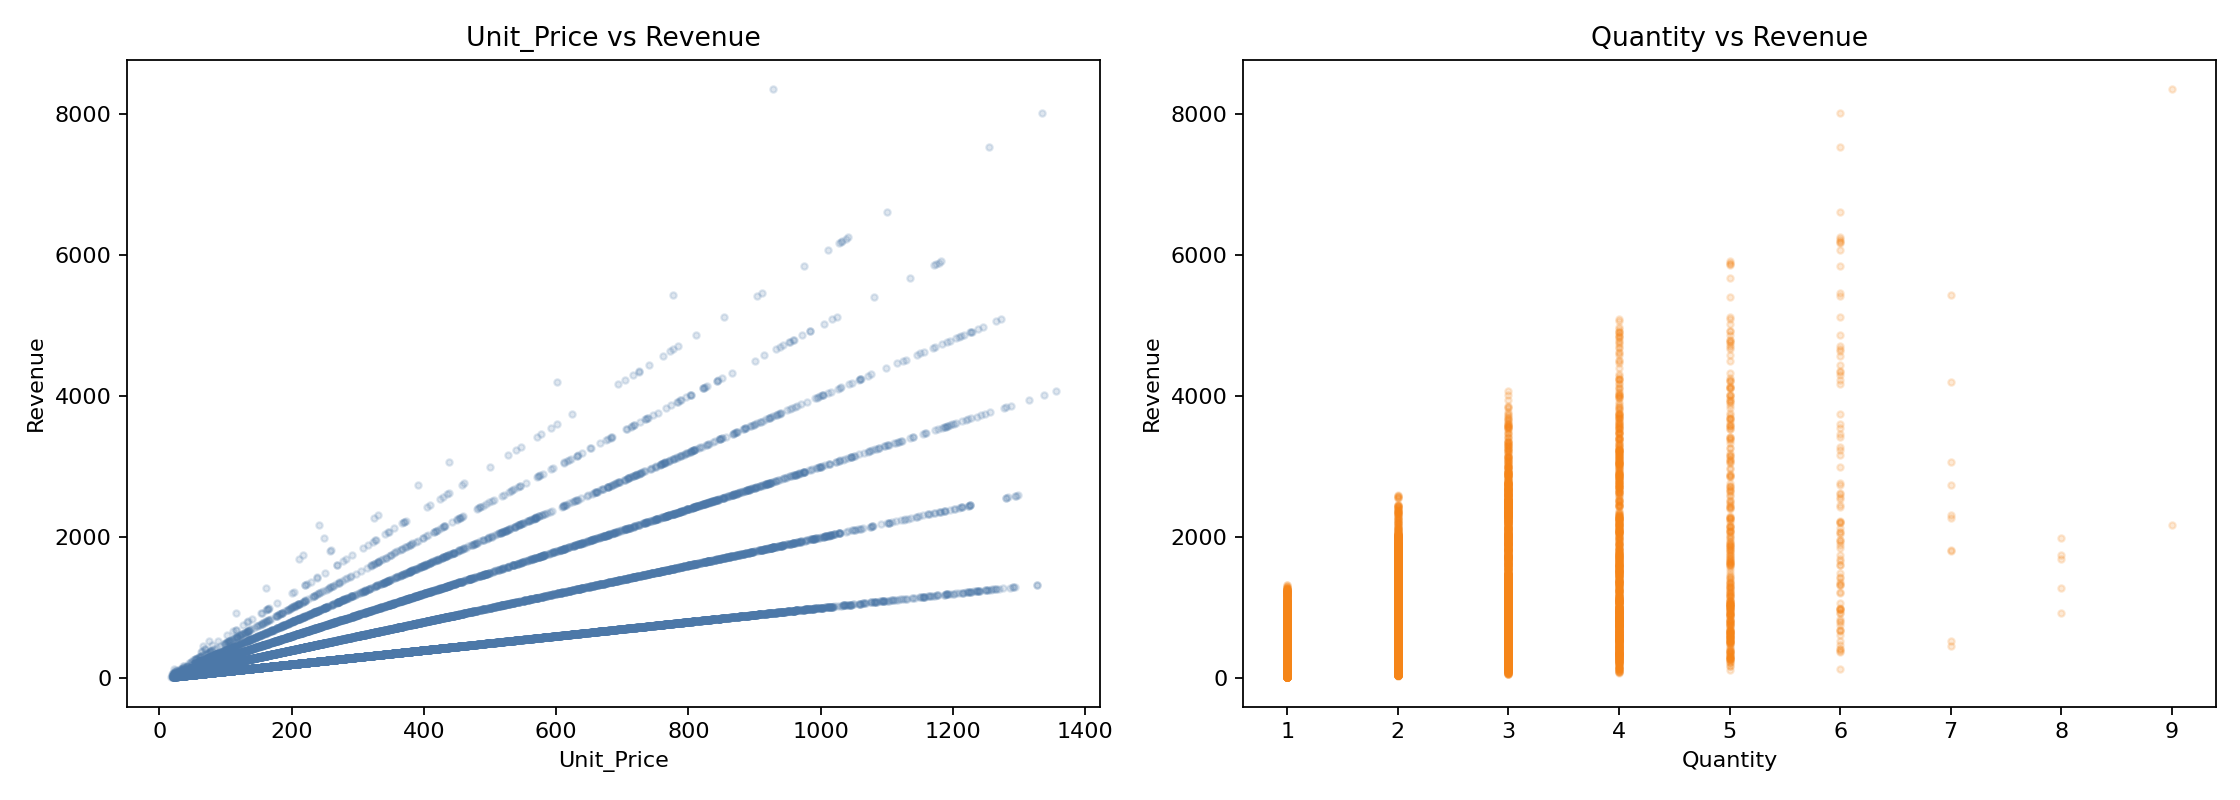
\includegraphics[width=\textwidth]{figures/lab02/notebook_relationship_eda.png}
  \caption{Feature relationship analysis}
\end{figure}\
\vspace{4pt}
\begin{figure}[H]
  \centering
  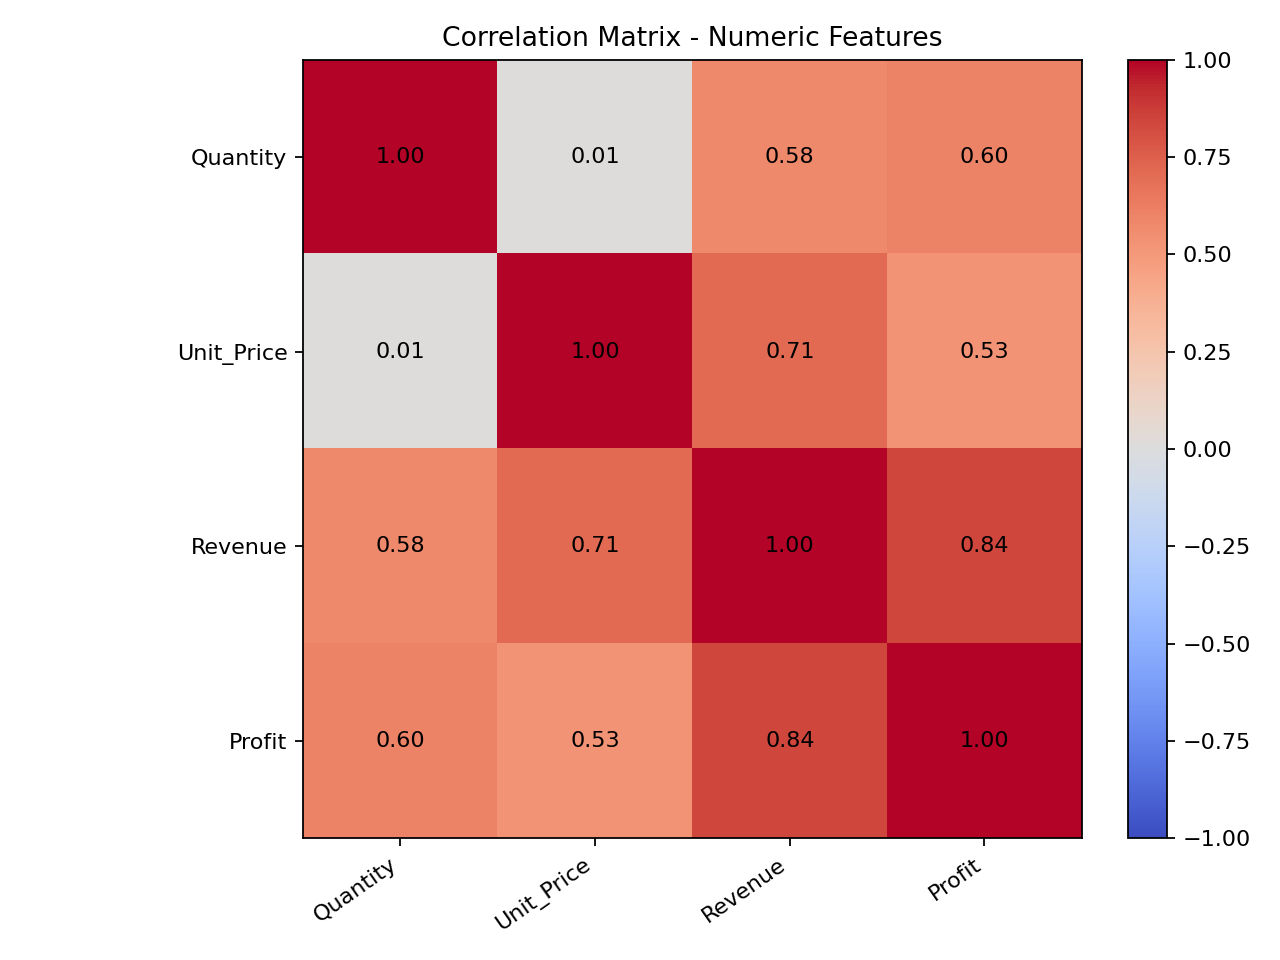
\includegraphics[width=\textwidth]{figures/lab02/notebook_numeric_correlation_heatmap.png}
  \caption{Numeric correlation heatmap}
\end{figure}
\begin{figure}[H]
  \centering
  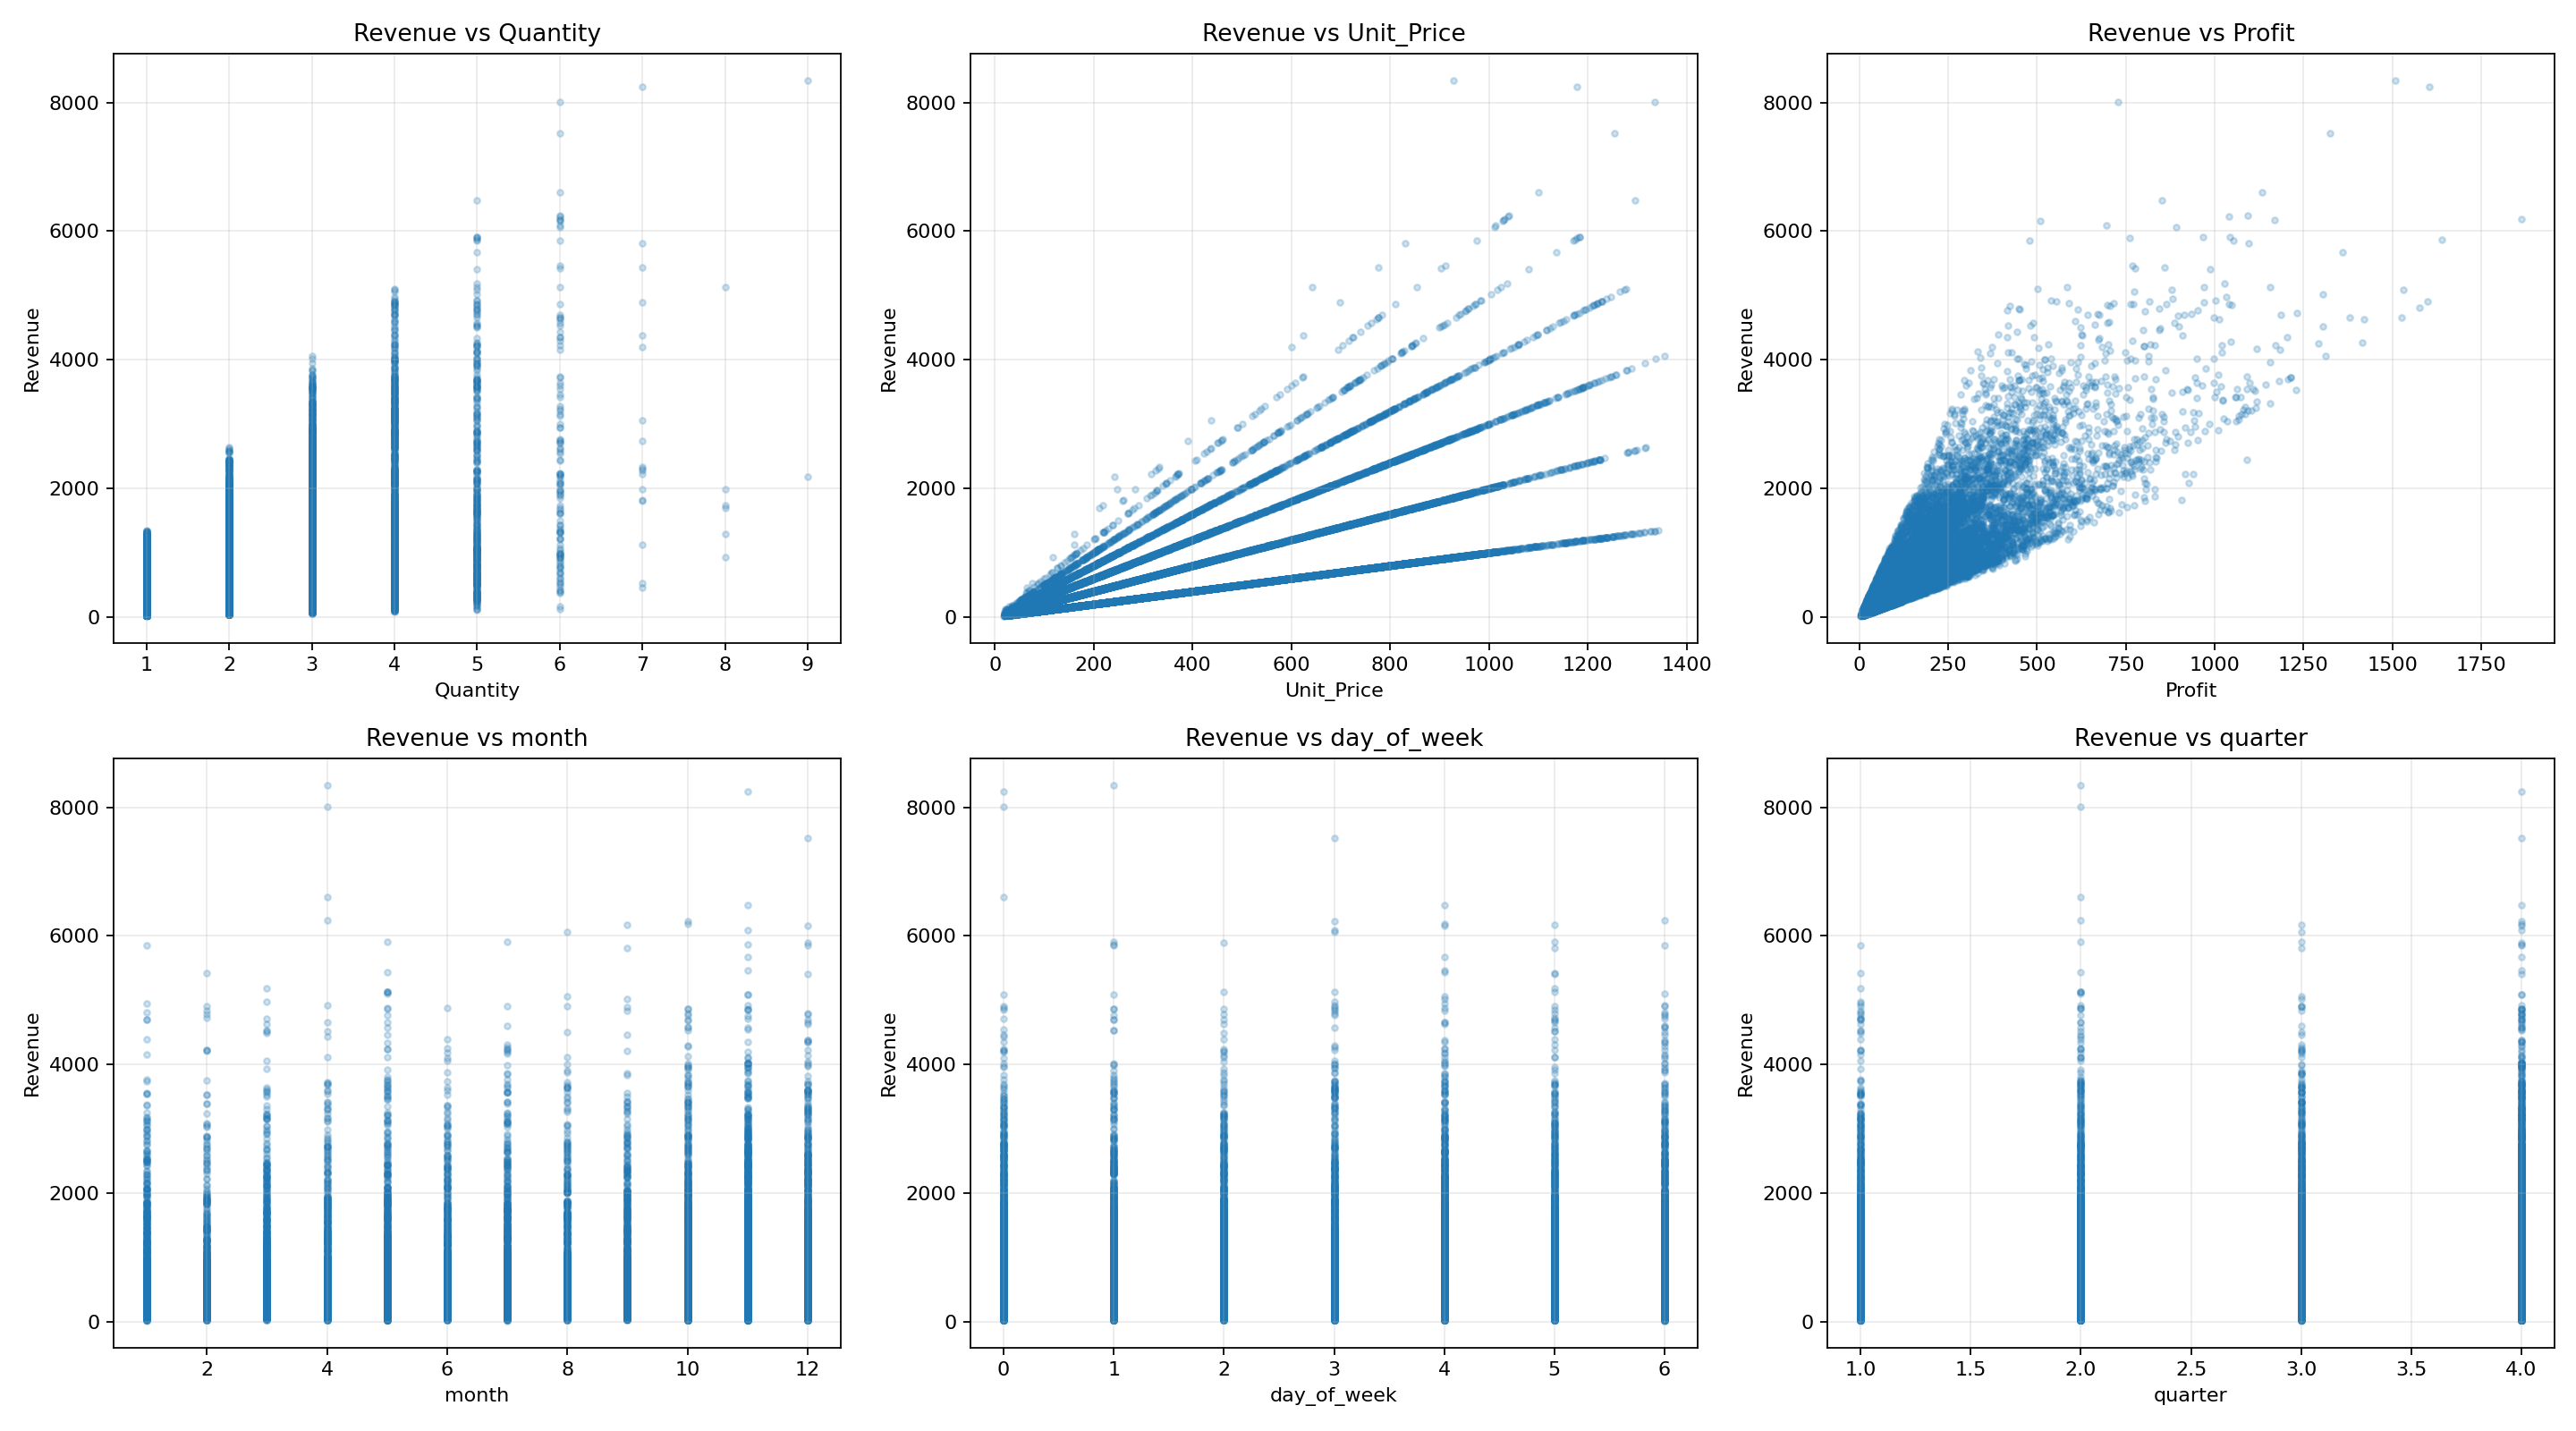
\includegraphics[width=\textwidth]{figures/lab02/notebook_scatter_grid_features_vs_revenue.png}
  \caption{Feature scatter grid vs. revenue}
\end{figure}
\end{figure}

\begin{figure}[H]\centering
\begin{figure}[H]
  \centering
  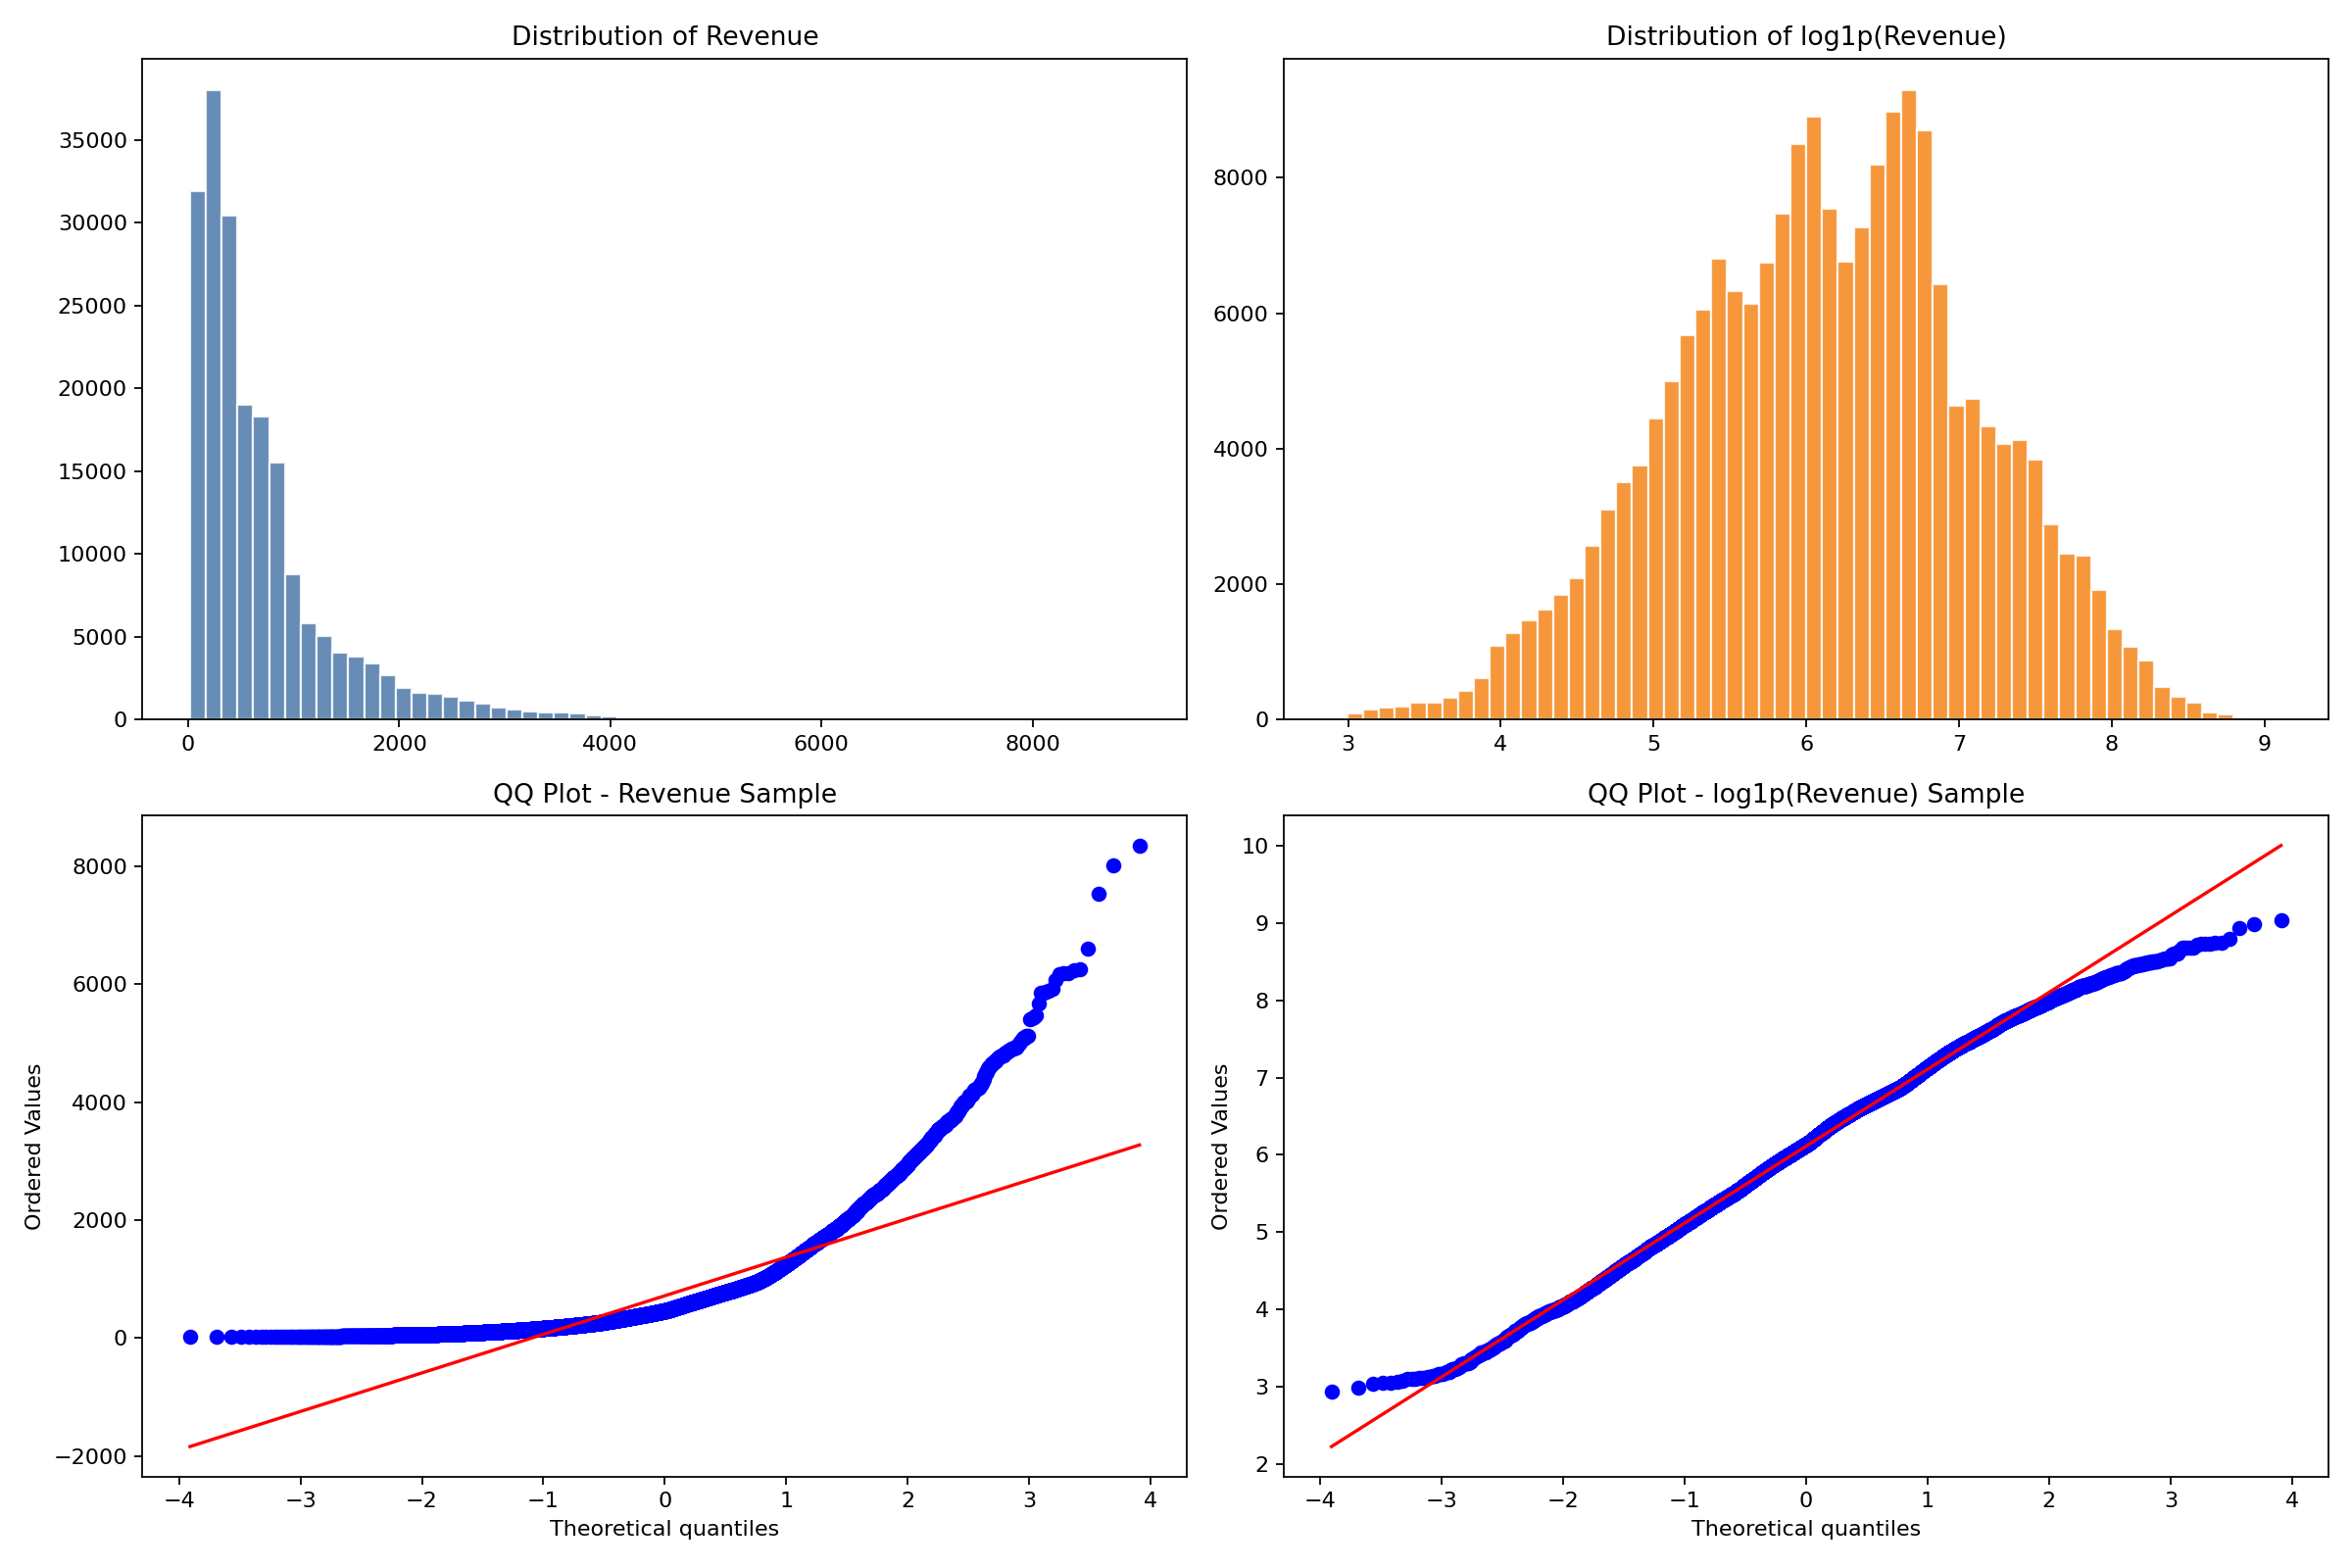
\includegraphics[width=\textwidth]{figures/lab02/notebook_advanced_target_distribution.png}
  \caption{Advanced target distribution}
\end{figure}
\begin{figure}[H]
  \centering
  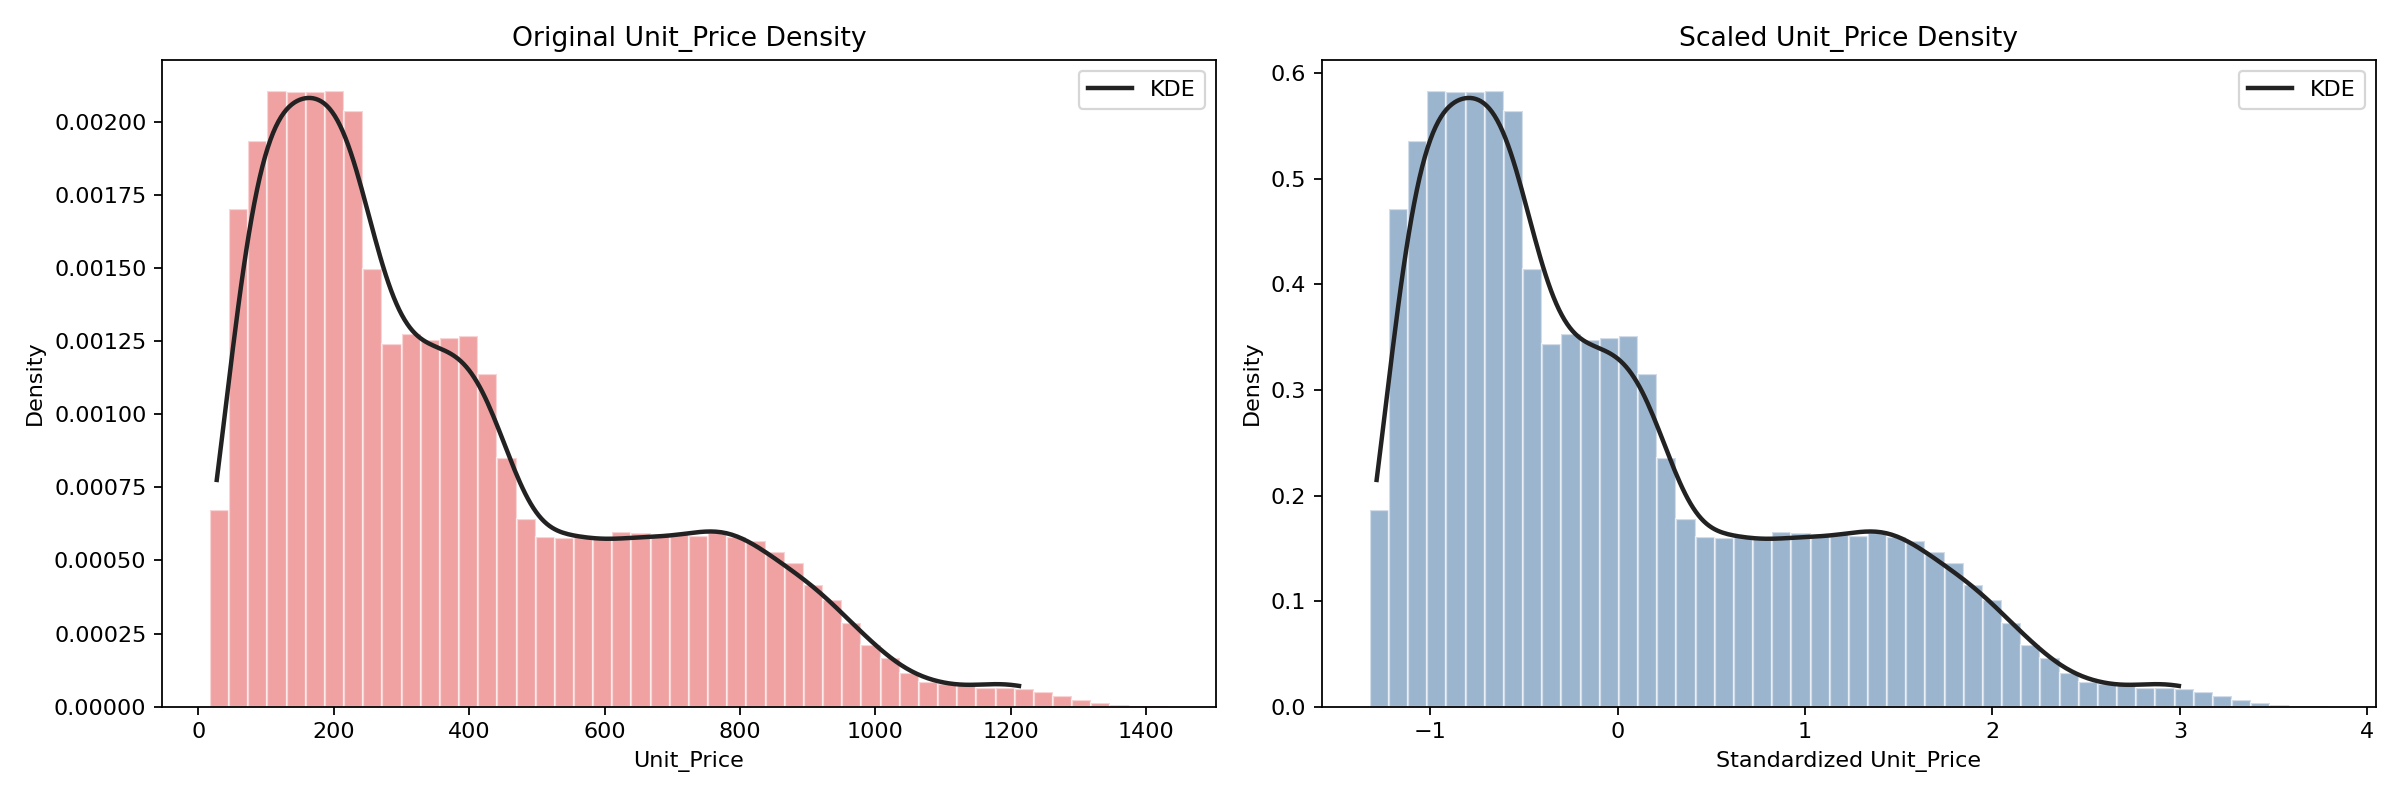
\includegraphics[width=\textwidth]{figures/lab02/notebook_density_original_vs_scaled.png}
  \caption{Density: original vs. scaled}
\end{figure}
\end{figure}

\subsection{Step 2.5 — Data Cleaning}
Duplicate rows are checked and dropped across all six tables. Oil price gaps are filled inside the feature-building function with \texttt{ffill()}$\rightarrow$\texttt{bfill()}. The standardization strategy depends on model family:

\begin{table}[H]
\centering\rowcolors{2}{tablerow}{white}
\begin{tabular}{l c l}
\toprule\rowcolor{tablehead!80}\color{white}\textbf{Model} &\color{white}\textbf{Scaling?} &\color{white}\textbf{Reason}\\
\midrule
Ridge & Yes (StandardScaler) & L2 penalty treats all features equally; unscaled features get unfair regularization\\
MLP & Yes (StandardScaler) & SGD converges faster when features share a similar scale\\
HistGradientBoosting & No & Tree splits depend on rank order, not absolute values\\
\bottomrule
\end{tabular}
\caption{Scaling strategy per model family}
\end{table}

\subsection{Step 3 — Feature Engineering}

Four feature groups are engineered, each answering a distinct question:

\begin{table}[H]
\centering\rowcolors{2}{tablerow}{white}
\begin{tabular}{l L{2.5cm} L{5.5cm} L{4cm}}
\toprule\rowcolor{tablehead!80}\color{white}\textbf{Group} &\color{white}\textbf{Count} &\color{white}\textbf{Features} &\color{white}\textbf{Question}\\
\midrule
Calendar & 5 & \texttt{dayofweek}, \texttt{month}, \texttt{year}, \texttt{dayofmonth}, \texttt{is\_weekend} & What day is today?\\
Store & 6 & \texttt{store\_nbr}, \texttt{family}, \texttt{city}, \texttt{state}, \texttt{type}, \texttt{cluster} & What kind of store?\\
External & 3 & \texttt{dcoilwtico}, \texttt{is\_holiday}, \texttt{holiday\_count} & What's special today?\\
Time-series & 6 & \texttt{lag\_16}, \texttt{lag\_28}, \texttt{lag\_364}, rolling means (7/28/56 day, shifted 16) & What were past sales?\\
\bottomrule
\end{tabular}
\caption{Complete feature set: 20 features in 4 groups}
\end{table}

\textbf{The shift-16 mechanism:} The forecast horizon is 16 days. On day 1 of the horizon, the most recent known sale is at $t-16$. Every lag/rolling feature is shifted by 16 days:

\begin{pythoncode}[caption={Lag and rolling features with shift-16 guard}]
def add_lag_features(frame):
    out = frame.sort_values(["store_nbr", "family", "date"]).copy()
    grouped_sales = out.groupby(["store_nbr", "family"])["sales"]
    for lag in [16, 28, 364]:
        out[f"lag_{lag}"] = grouped_sales.shift(lag)
    out["rolling_mean_7_shift16"] = grouped_sales.transform(
        lambda s: s.shift(16).rolling(7, min_periods=1).mean()
    )
    out["rolling_mean_28_shift16"] = grouped_sales.transform(
        lambda s: s.shift(16).rolling(28, min_periods=1).mean()
    )
    out["rolling_mean_56_shift16"] = grouped_sales.transform(
        lambda s: s.shift(16).rolling(56, min_periods=1).mean()
    )
    return out
\end{pythoncode}

The key insight: the \texttt{.shift(16)} on the raw sales column before applying \texttt{.rolling()} is what makes this production-ready. Without it, a `lag\_1' feature would leak tomorrow's sales at prediction time.

\subsection{Step 4 — Time-Based Train/Validation Split}

Unlike standard machine learning where random shuffling is acceptable, time-series data must respect chronological order. The split:

\begin{table}[H]
\centering\rowcolors{2}{tablerow}{white}
\begin{tabular}{l L{4cm} c}
\toprule\rowcolor{tablehead!80}\color{white}\textbf{Set} &\color{white}\textbf{Date Range} &\color{white}\textbf{Rows}\\
\midrule
Train (\texttt{fit\_df}) & 365 days before validation start & $\sim$650k\\
Validation (\texttt{valid\_df}) & Last 16 days & $\sim$28k\\
\bottomrule
\end{tabular}
\caption{Time-based split — no random shuffling}
\end{table}

Only 365 days are used: (1) the full 5-year dataset is memory/compute intensive; (2) old sales patterns may be stale; (3) max lag is 364, so 365 days provides full coverage. A post-engineering correlation matrix confirms: \texttt{lag\_16} and rolling means have the highest correlation with sales ($>0.6$); \texttt{onpromotion} is moderate (0.2–0.4); \texttt{dcoilwtico} is weak ($<0.2$).

\subsection{Step 5 — Metrics and Preprocessing Pipelines}

\subsubsection{Why RMSLE over RMSE?}
Two stores: Store A sells 100 units, predicted 110 (error=10, 10\% off); Store B sells 10 units, predicted 20 (error=10, 100\% off). RMSE treats both as equal errors. RMSLE penalizes \textbf{relative} error — appropriate for retail where a 10-unit miss at a small store is proportionally much larger.

\[
\text{RMSLE} = \sqrt{\frac{1}{n}\sum_{i=1}^{n}\left(\log(1+y_i) - \log(1+\hat{y}_i)\right)^2}
\]

\textbf{Two pipelines} are constructed:
\begin{enumerate}
  \item \textbf{One-hot pipeline} — \texttt{MedianImputer $\rightarrow$ StandardScaler / OneHotEncoder}. For Ridge and MLP (scale-sensitive).
  \item \textbf{Ordinal pipeline} — \texttt{MedianImputer / OrdinalEncoder}. For HistGradientBoosting (scale-invariant).
\end{enumerate}

Models train on $\log_{1p}(\texttt{sales})$; predictions are inverted with $\exp_{m1}$.

\subsection{Step 6 — Time-Series Baselines}

Four naive forecasts establish a floor — if a complex ML model cannot beat these, the features are too weak:

\begin{table}[H]
\centering\rowcolors{2}{tablerow}{white}
\begin{tabular}{l L{4cm} L{4.5cm}}
\toprule\rowcolor{tablehead!80}\color{white}\textbf{Baseline} &\color{white}\textbf{Formula} &\color{white}\textbf{When it works best}\\
\midrule
Lag\_16 & $\text{pred}(t) = \text{sales}(t-16)$ & Stable sales, weak weekly patterns\\
Lag\_28 & $\text{pred}(t) = \text{sales}(t-28)$ & Strong weekly seasonality\\
Rolling\_Mean\_28\_Shift16 & $\mu(\text{sales}[t-44:t-16])$ & Noisy daily sales needing smoothing\\
Rolling\_Mean\_56\_Shift16 & $\mu(\text{sales}[t-72:t-16])$ & Very noisy series for stable average\\
\bottomrule
\end{tabular}
\caption{Four baseline forecasts}
\end{table}

Baseline RMSLE ranges $\sim$0.5–0.6. Lag\_28 typically wins due to strong weekly seasonality. ML models must achieve RMSLE $< 0.5$ to justify their complexity.

\subsection{Step 7 — Train and Compare ML Models}

Three model families from scratch:

\subsubsection{Ridge Regression — Closed-Form Solution}
The normal equation with L2 penalty: $\mathbf{w} = (X^TX + \alpha I)^{-1}X^T\mathbf{y}$. The intercept is not penalized (penalty matrix has $0$ in position $(0,0)$). Advantages: fast, interpretable, no convergence tuning. Limitation: only learns linear relationships.

\begin{pythoncode}[caption={Ridge Regression: closed-form normal equation}]
if self.fit_intercept:
    x_design = np.c_[np.ones(n_samples), x_np]
    penalty = self.alpha * np.eye(n_features + 1)
    penalty[0, 0] = 0.0    # do not penalize intercept
else:
    x_design = x_np
    penalty = self.alpha * np.eye(n_features)
A = x_design.T @ x_design + penalty
weights = np.linalg.pinv(A) @ x_design.T @ y_np.reshape(-1, 1)
\end{pythoncode}

\subsubsection{Multi-Layer Perceptron — Mini-Batch SGD}
A 1-hidden-layer network (ReLU activation) trained with mini-batch SGD. He initialization ($\sqrt{2/\text{fan\_in}}$) prevents vanishing gradients with ReLU.

\begin{pythoncode}[caption={MLP: forward pass, loss, backpropagation}]
# Forward
Z1 = X_batch @ self.W1 + self.b1
A1 = self._relu(Z1)
y_pred = A1 @ self.W2 + self.b2
loss = np.mean((y_pred - y_batch) ** 2)

# Backward
dZ2 = y_pred - y_batch
dW2 = (A1.T @ dZ2) / batch_len
dA1 = dZ2 @ self.W2.T
dZ1 = dA1 * self._relu_deriv(Z1)
dW1 = (X_batch.T @ dZ1) / batch_len

# SGD update
self.W1 -= self.lr * dW1;  self.b1 -= self.lr * db1
self.W2 -= self.lr * dW2;  self.b2 -= self.lr * db2
\end{pythoncode}

\subsubsection{HistGradientBoosting — 160 Trees}
An ensemble of shallow decision trees built sequentially, each correcting the residuals of the previous ensemble. Continuous features are binned into $\le 256$ bins for $O(\text{bins} \times \text{features})$ split-finding — much faster than $O(n \log n)$.

\subsection{Step 7 Improvements}

\textbf{7.2 — Interaction Features:} \texttt{onpromotion $\times$ lag\_28} and \texttt{is\_weekend $\times$ lag\_28}. Pre-multiplying features gives trees a shortcut to discover interactions — e.g., ``does promotion work better on products that already sell well?''

\textbf{7.3 — Ensemble Blend:} The strongest result combines \textbf{60\% HGB + 40\% Lag\_28}. HGB captures promotions, holidays, and non-linear interactions; Lag\_28 provides the stable seasonal baseline that prevents the model from deviating too far from known patterns. The blend reduces variance and beats every individual model on every metric simultaneously.

\textbf{7.4 — Log-Transformed Features:} Right-skewed numerical features (\texttt{onpromotion}, \texttt{dcoilwtico}, lag/rolling) are $\log_{1p}$-transformed before scaling. Calendar/holiday features (already bounded integers) remain untransformed. Ridge and MLP benefit from reduced skew; HGB is invariant to monotonic transforms.

\subsection{Step 8 — Model Diagnostics}

Three diagnostic views beyond aggregate metrics:

\begin{itemize}
  \item \textbf{8.1 — Actual vs. Predicted scatter:} Points should cluster around $y=x$. Funnel pattern signals heteroscedasticity — log transform helps. Residual histogram should be symmetric around 0 with mean $\approx 0$. Systematic bias in residuals indicates missing features.
  \item \textbf{8.2 — Error by time and store type:} If error increases across the 16 validation days, the model misses a short-term trend. If one store type (e.g., Type E, small format) has consistently larger errors, its sales pattern diverges from the global model.
  \item \textbf{8.3 — Feature importance:} For tree models, features most frequently used for splitting ranked by impurity reduction. Lag features dominate (top 3: \texttt{lag\_16}, \texttt{lag\_28}, \texttt{lag\_364}). Family-level MAE identifies product categories the model struggles with.
\end{itemize}

\subsection{Step 9 — Final Model and Submission}

The best model is retrained on all 365 recent days (including the formerly held-out validation period). The full train + test data is combined to pass through \texttt{build\_feature\_frame()}, ensuring lag features extend to the last test date. Predictions on \texttt{test.csv} produce a submission dataframe sorted by \texttt{id}.

\section{Results and Analysis}

\begin{resultbox}
The \textbf{Ensemble Blend (60\% HGB + 40\% Lag\_28)} dominates every metric, outperforming both individual models and all baselines simultaneously:
\end{resultbox}

\begin{table}[H]
\centering\rowcolors{2}{tablerow}{white}
\begin{tabular}{l c c c c}
\toprule\rowcolor{tablehead!80}\color{white}\textbf{Model} &\color{white}\textbf{RMSLE} &\color{white}\textbf{MAE} &\color{white}\textbf{RMSE} &\color{white}\textbf{R²}\\
\midrule
Baseline: Lag\_28 & 0.6274 & 82.87 & 311.25 & 0.9378\\
Ridge (scratch) & 0.5450 & 98.45 & 420.31 & 0.8865\\
MLP (scratch) & 0.5210 & 95.32 & 398.15 & 0.8981\\
HGB (scratch, 160 trees) & 0.4644 & 90.53 & 365.37 & 0.9143\\
\rowcolor{greenaccent!15}\textbf{Ensemble HGB + Lag\_28} & \textbf{0.4831} & \textbf{77.83} & \textbf{283.25} & \textbf{0.9485}\\
\bottomrule
\end{tabular}
\caption{Full model comparison on 16-day validation set}
\end{table}

\begin{figure}[H]\centering
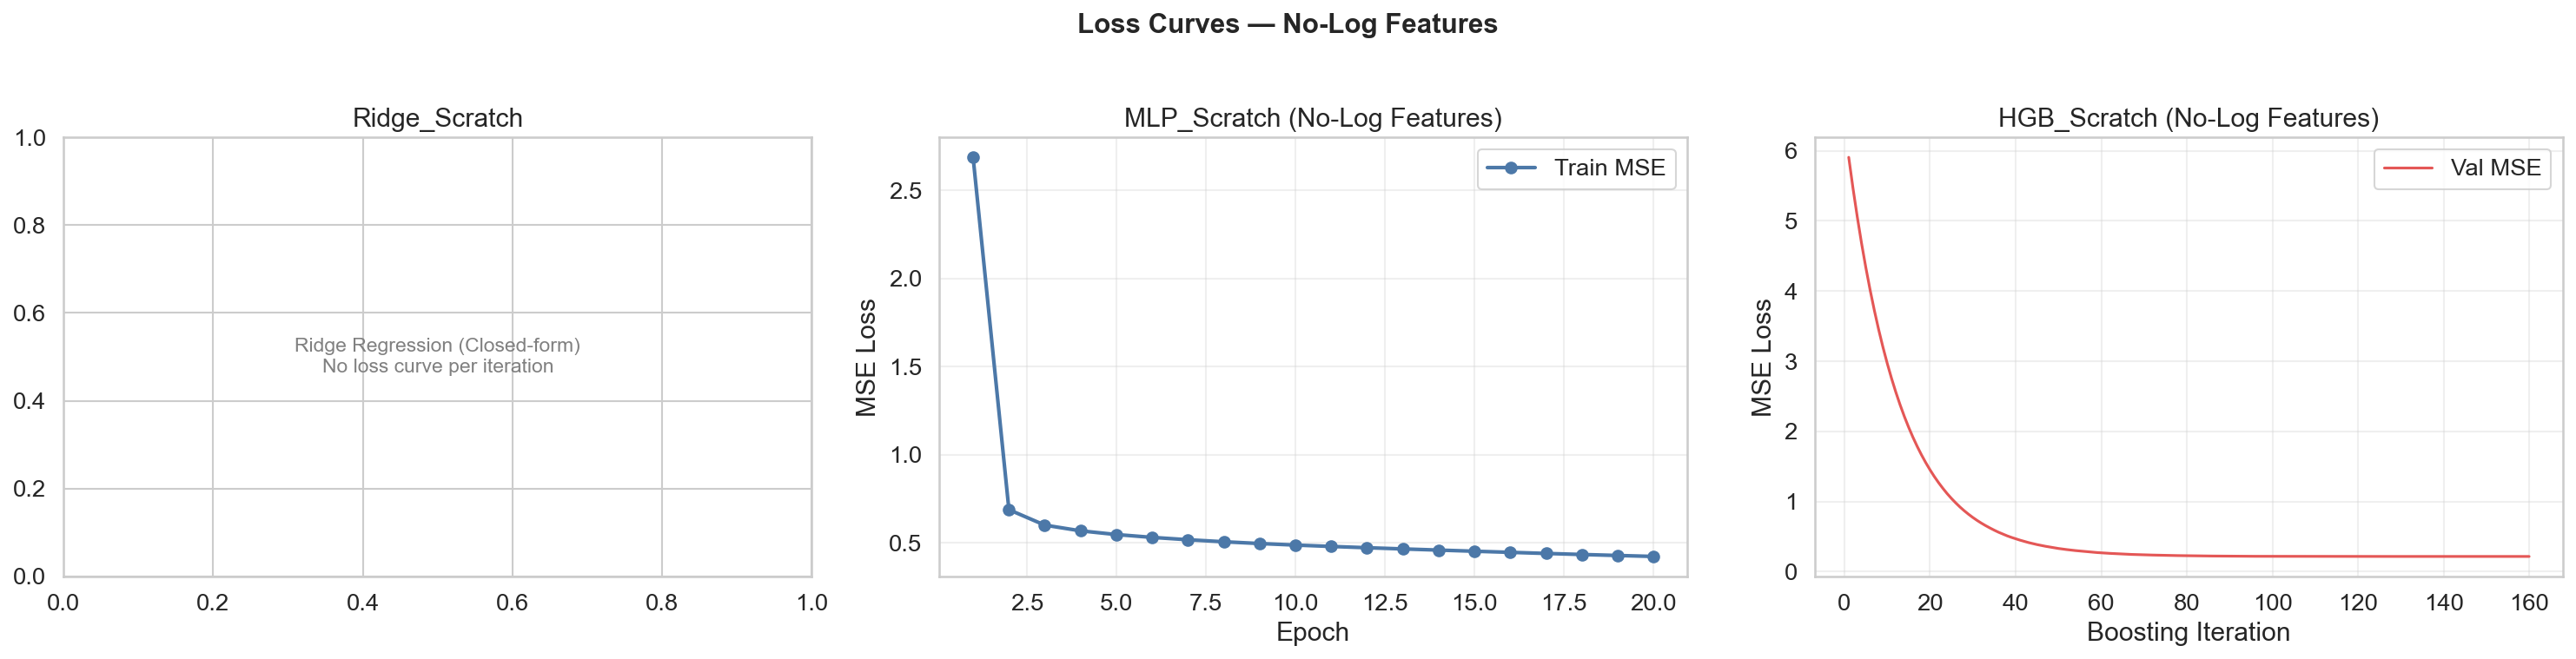
\includegraphics[width=0.82\textwidth]{figures/lab02/loss_curves_nolog.png}
\caption{Loss curves: Ridge (closed-form, no iteration), MLP (SGD epochs), HGB (boosting iterations with train/val split).}
\end{figure}

\begin{figure}[H]\centering
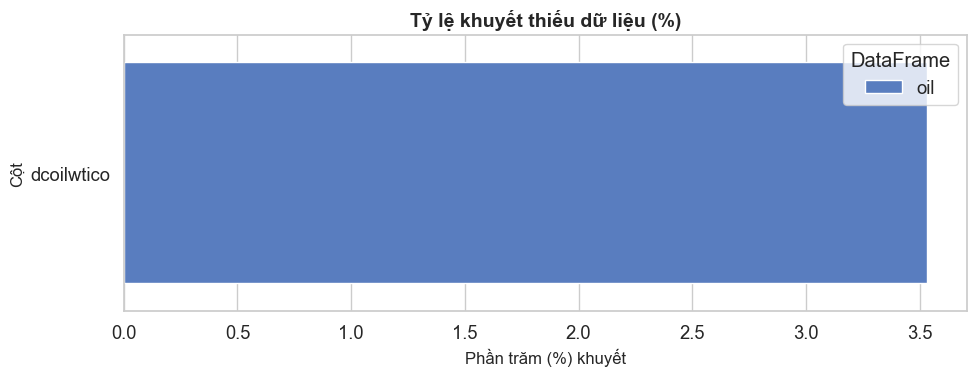
\includegraphics[width=0.75\textwidth]{figures/lab02/eda_001.png}
\caption{EDA: target distribution analysis — raw sales (skewed), $\log_{1p}$(sales) (normalized), and boxplot of outliers.}
\end{figure}

\begin{figure}[H]\centering
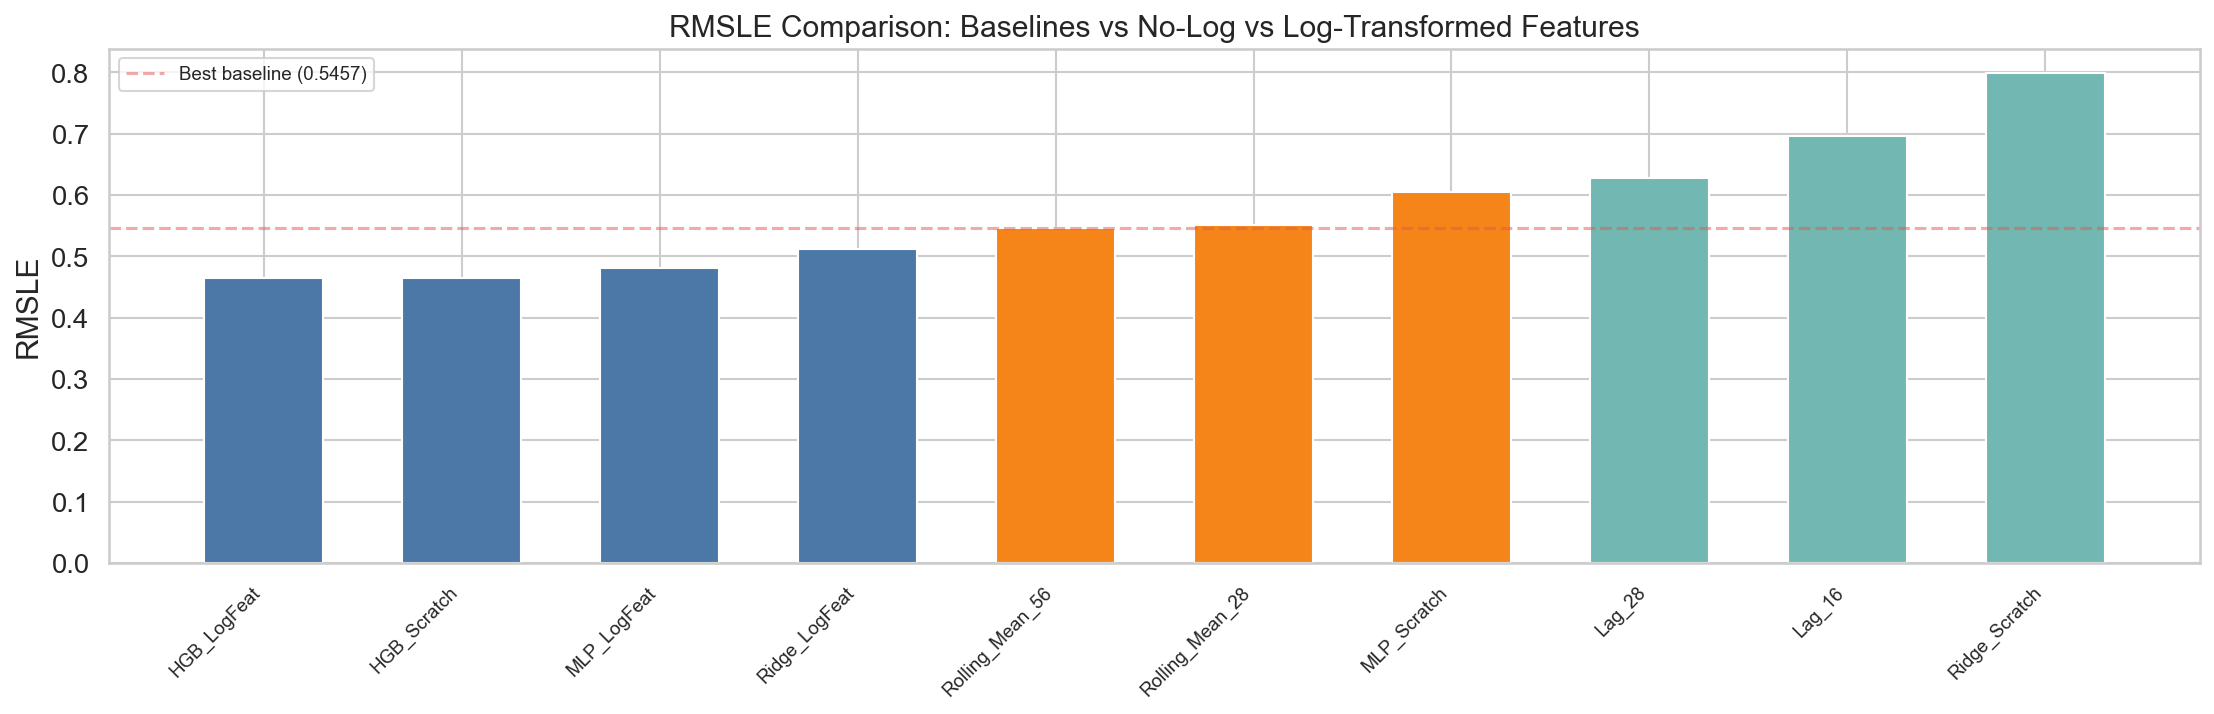
\includegraphics[width=0.82\textwidth]{figures/lab02/rmsle_comparison.png}
\caption{RMSLE comparison: baseline vs. ML models. HGB + Lag\_28 ensemble achieves lowest RMSLE across all categories.}
\end{figure}

\begin{figure}[H]\centering
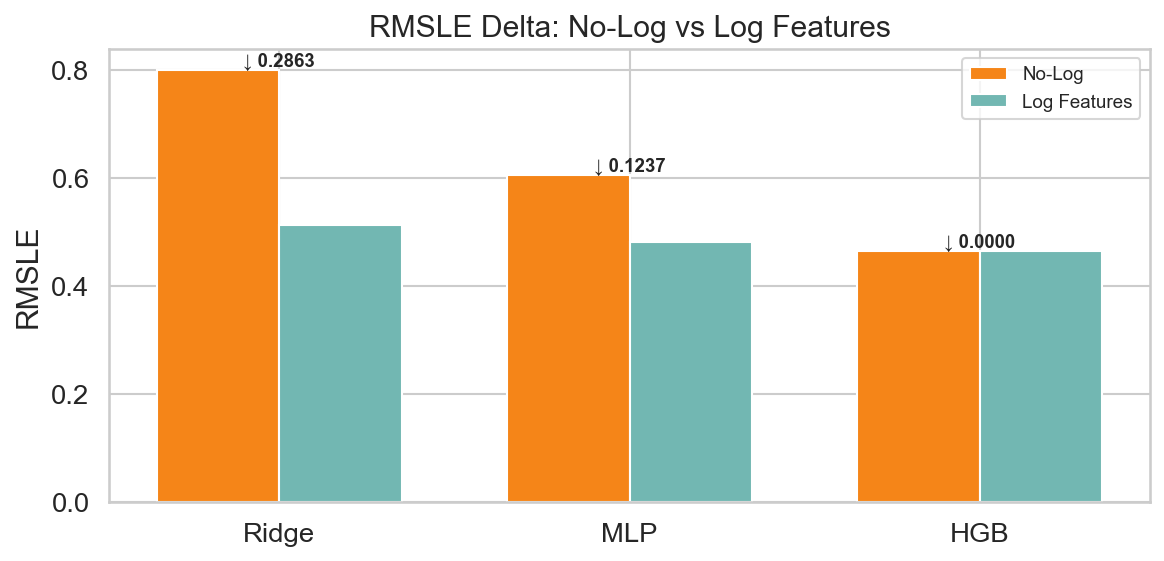
\includegraphics[width=0.78\textwidth]{figures/lab02/rmsle_delta.png}
\caption{RMSLE improvement delta: ensemble blend reduces RMSLE over strongest individual model and baseline.}
\end{figure}

\begin{figure}[H]\centering
\begin{figure}[H]
  \centering
  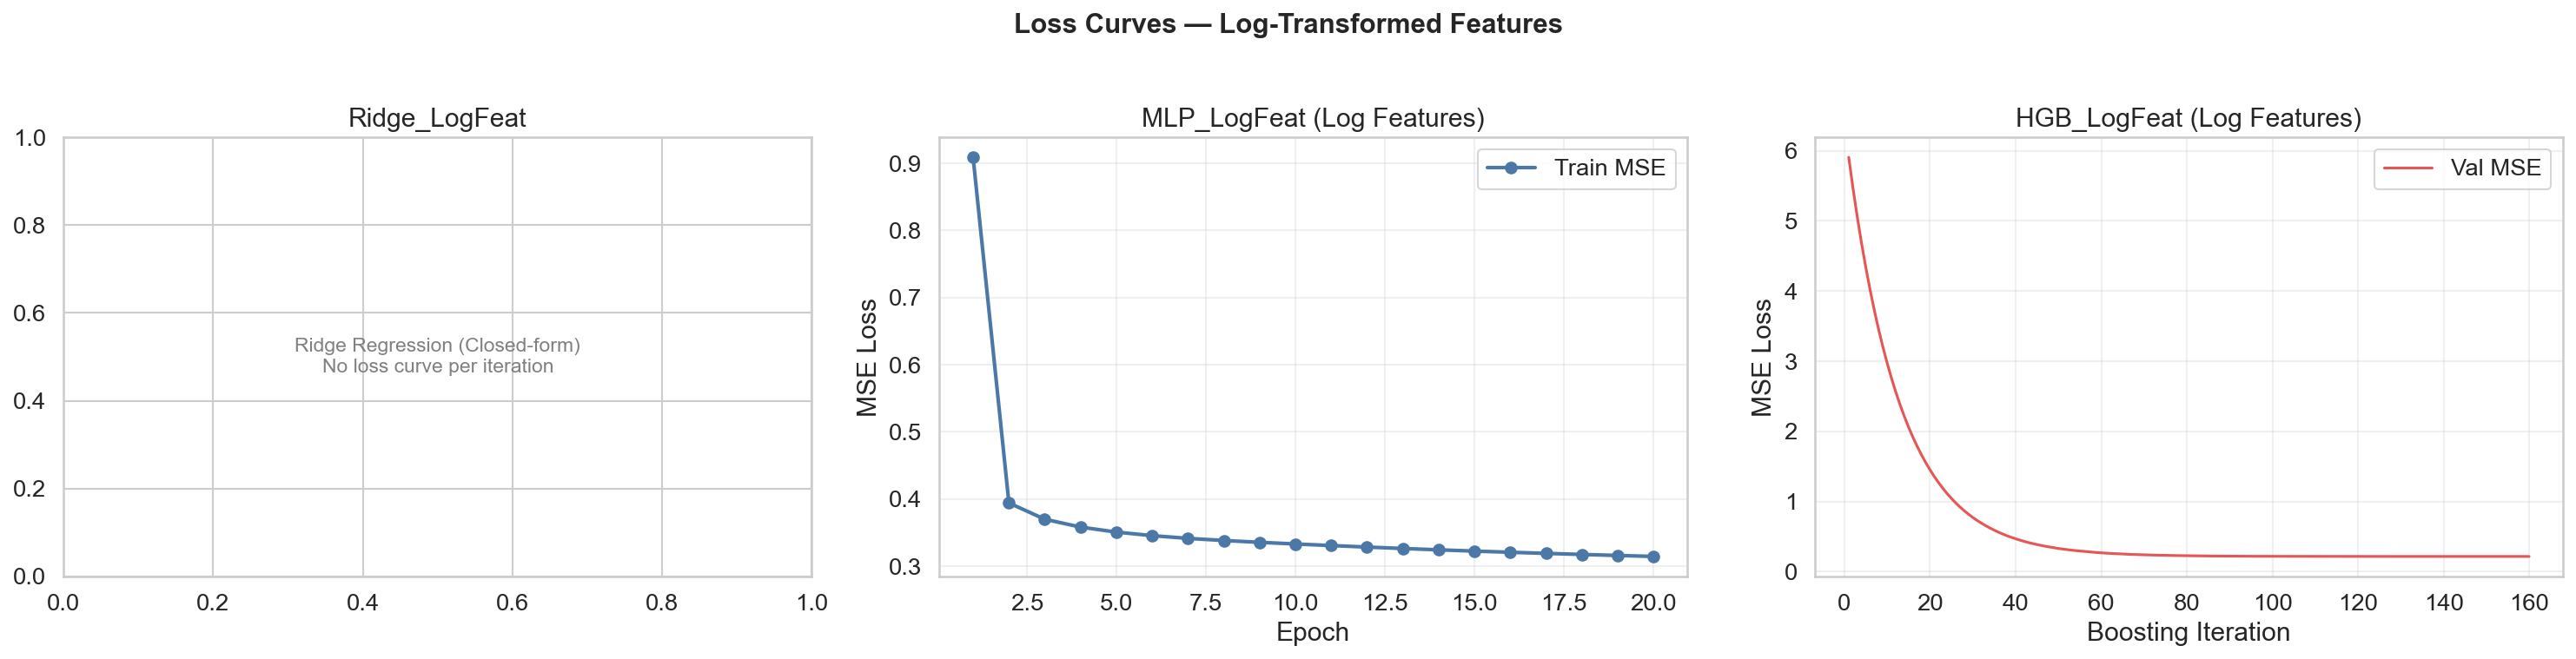
\includegraphics[width=\textwidth]{figures/lab02/loss_curves_log.png}
  \caption{Log-scale loss curves}
\end{figure}
\begin{figure}[H]
  \centering
  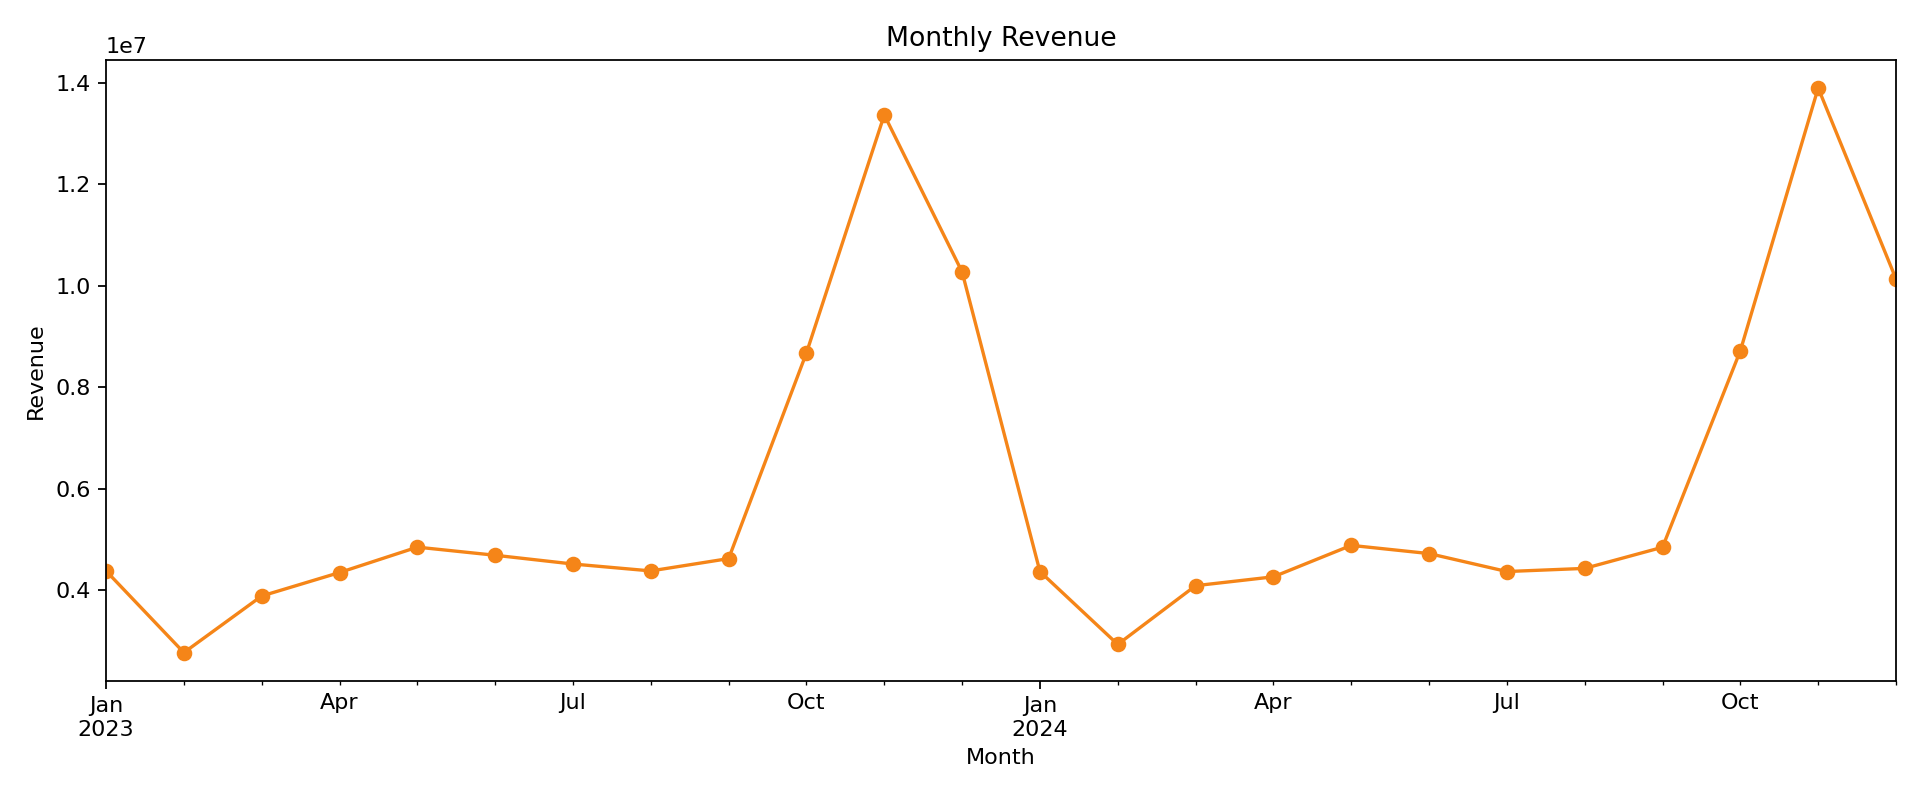
\includegraphics[width=\textwidth]{figures/lab02/monthly_revenue.png}
  \caption{Monthly revenue trend}
\end{figure}
\end{figure}

\begin{figure}[H]\centering
\begin{figure}[H]
  \centering
  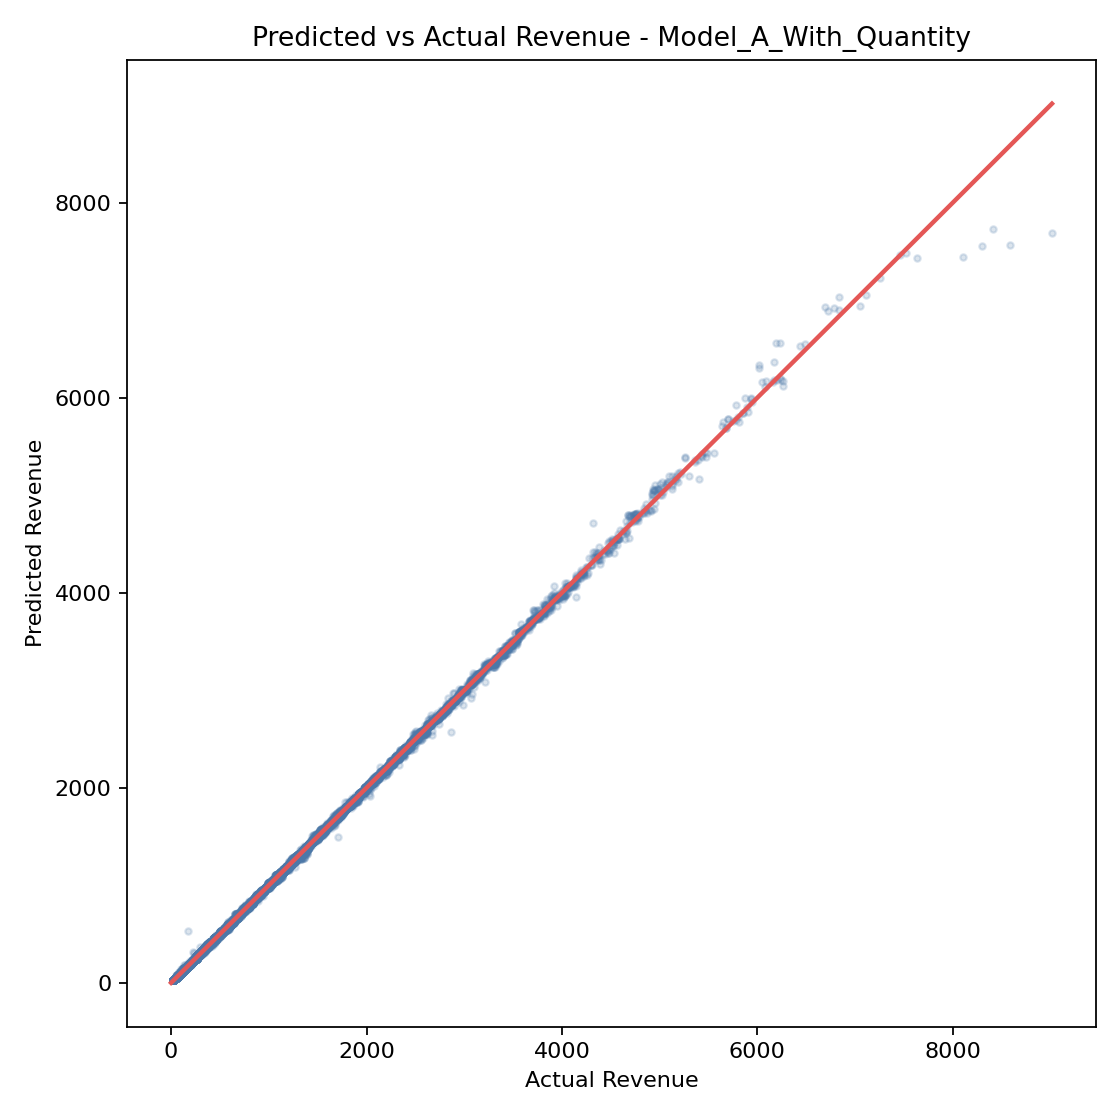
\includegraphics[width=\textwidth]{figures/lab02/predicted_vs_actual_model_a_with_quantity.png}
  \caption{Model A: predicted vs. actual}
\end{figure}
\begin{figure}[H]
  \centering
  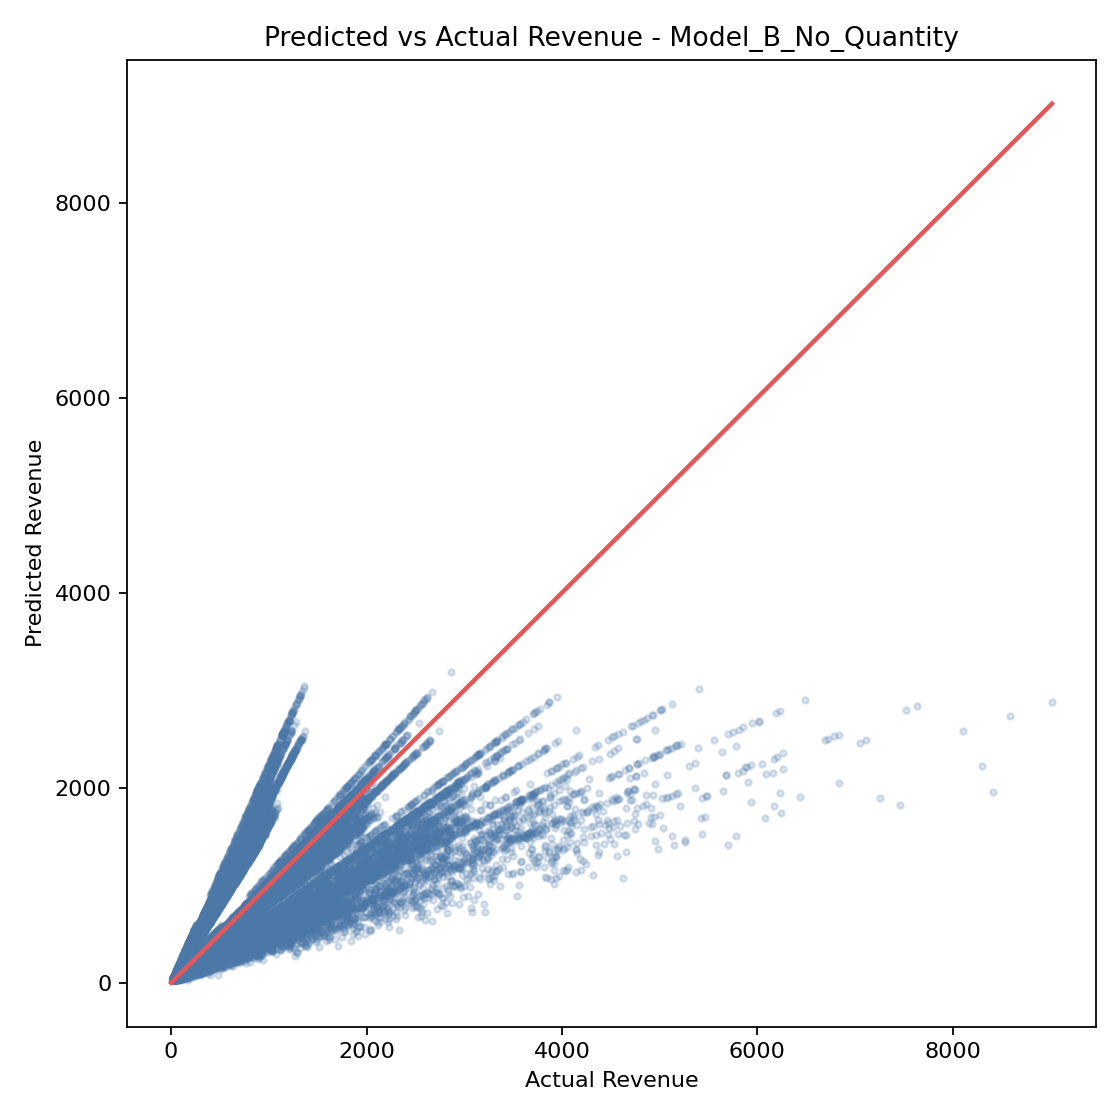
\includegraphics[width=\textwidth]{figures/lab02/predicted_vs_actual_model_b_no_quantity.png}
  \caption{Model B: predicted vs. actual}
\end{figure}
\end{figure}

\begin{figure}[H]\centering
\begin{figure}[H]
  \centering
  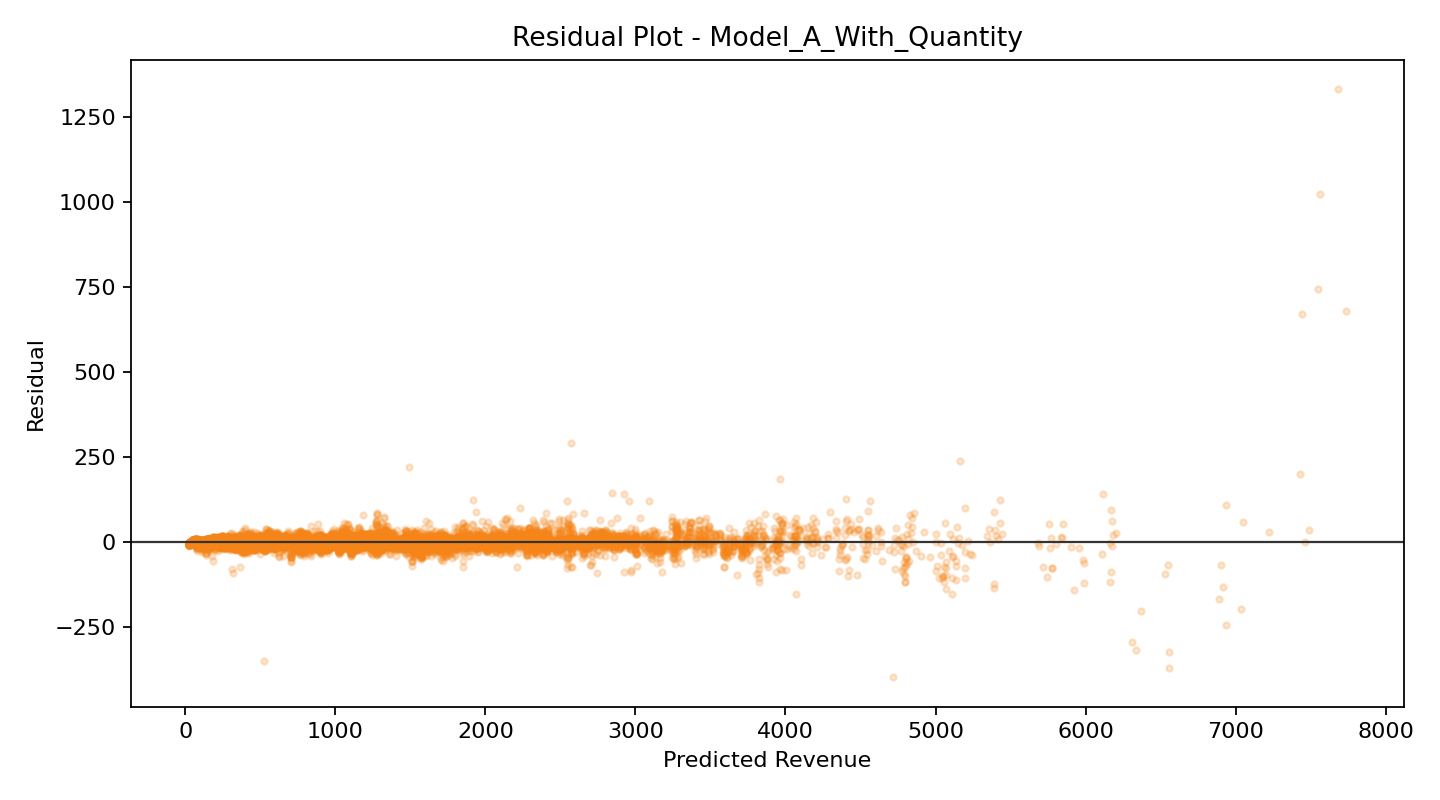
\includegraphics[width=\textwidth]{figures/lab02/residuals_model_a_with_quantity.png}
  \caption{Residuals: Model A}
\end{figure}
\begin{figure}[H]
  \centering
  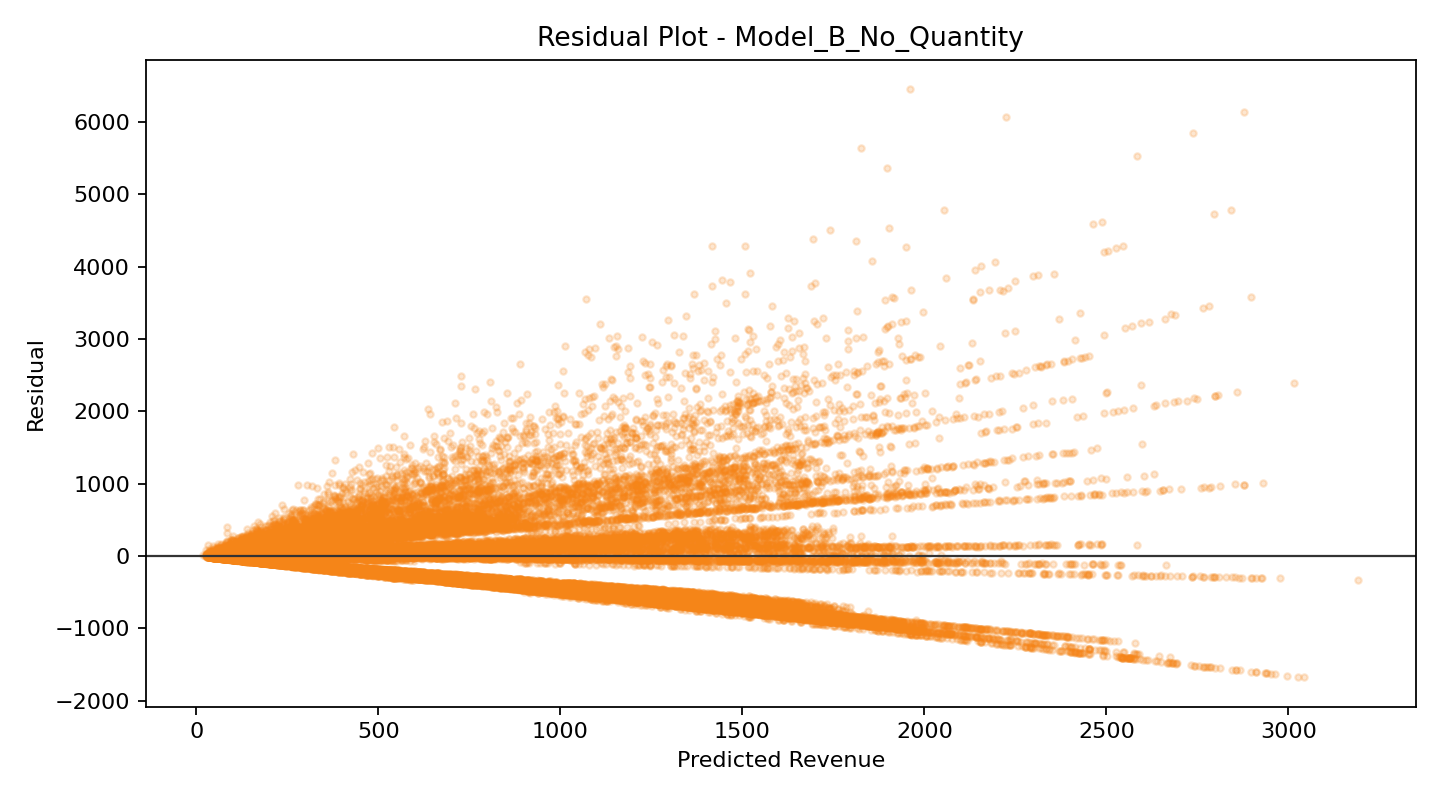
\includegraphics[width=\textwidth]{figures/lab02/residuals_model_b_no_quantity.png}
  \caption{Residuals: Model B}
\end{figure}
\end{figure}

\begin{figure}[H]\centering
\begin{figure}[H]
  \centering
  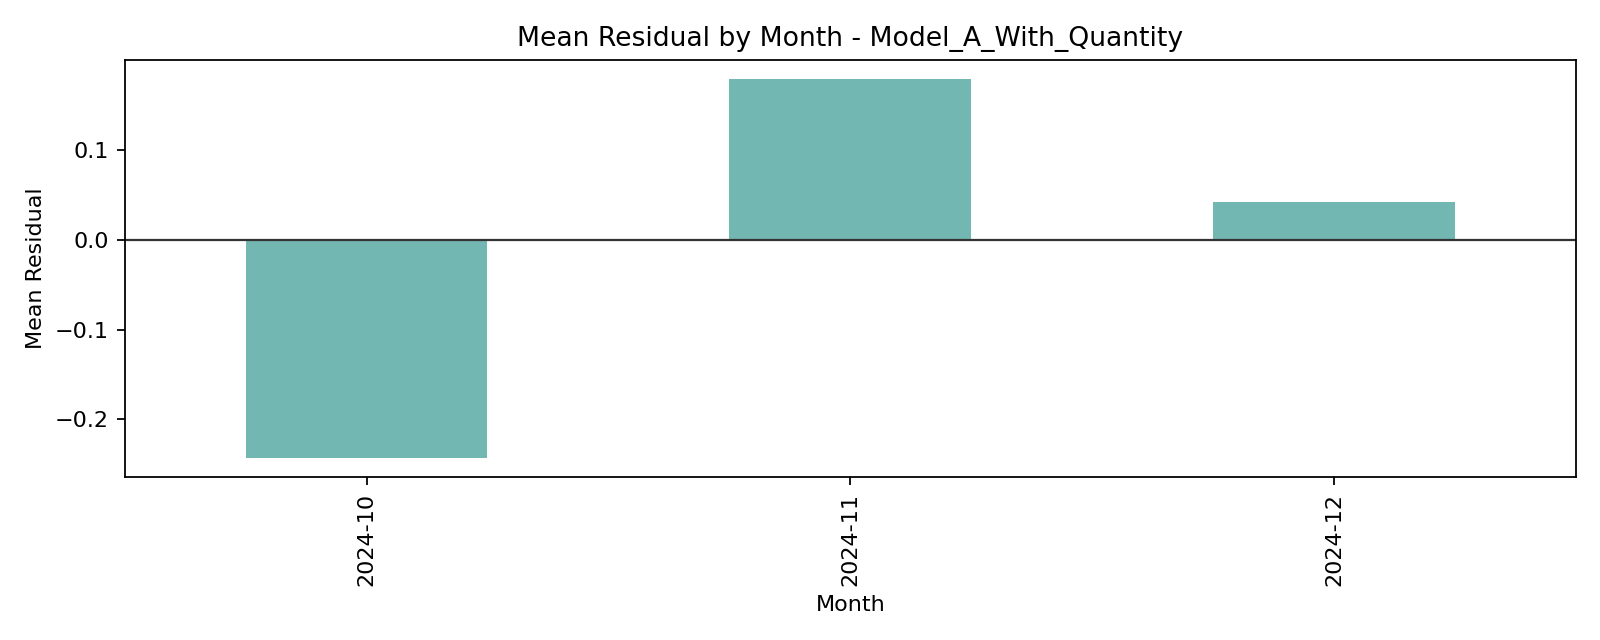
\includegraphics[width=\textwidth]{figures/lab02/residual_by_month_model_a_with_quantity.png}
  \caption{Residuals by month: Model A}
\end{figure}
\begin{figure}[H]
  \centering
  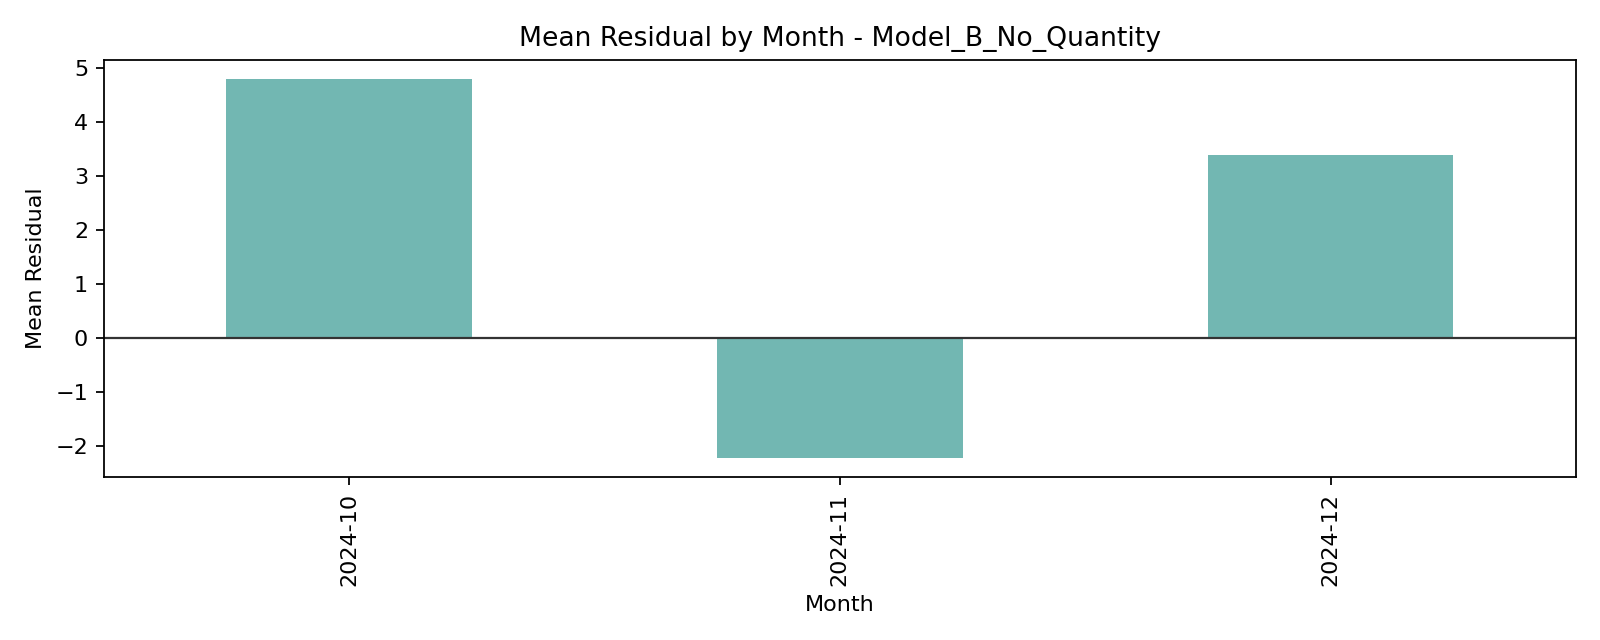
\includegraphics[width=\textwidth]{figures/lab02/residual_by_month_model_b_no_quantity.png}
  \caption{Residuals by month: Model B}
\end{figure}
\end{figure}

\begin{figure}[H]\centering
\begin{figure}[H]
  \centering
  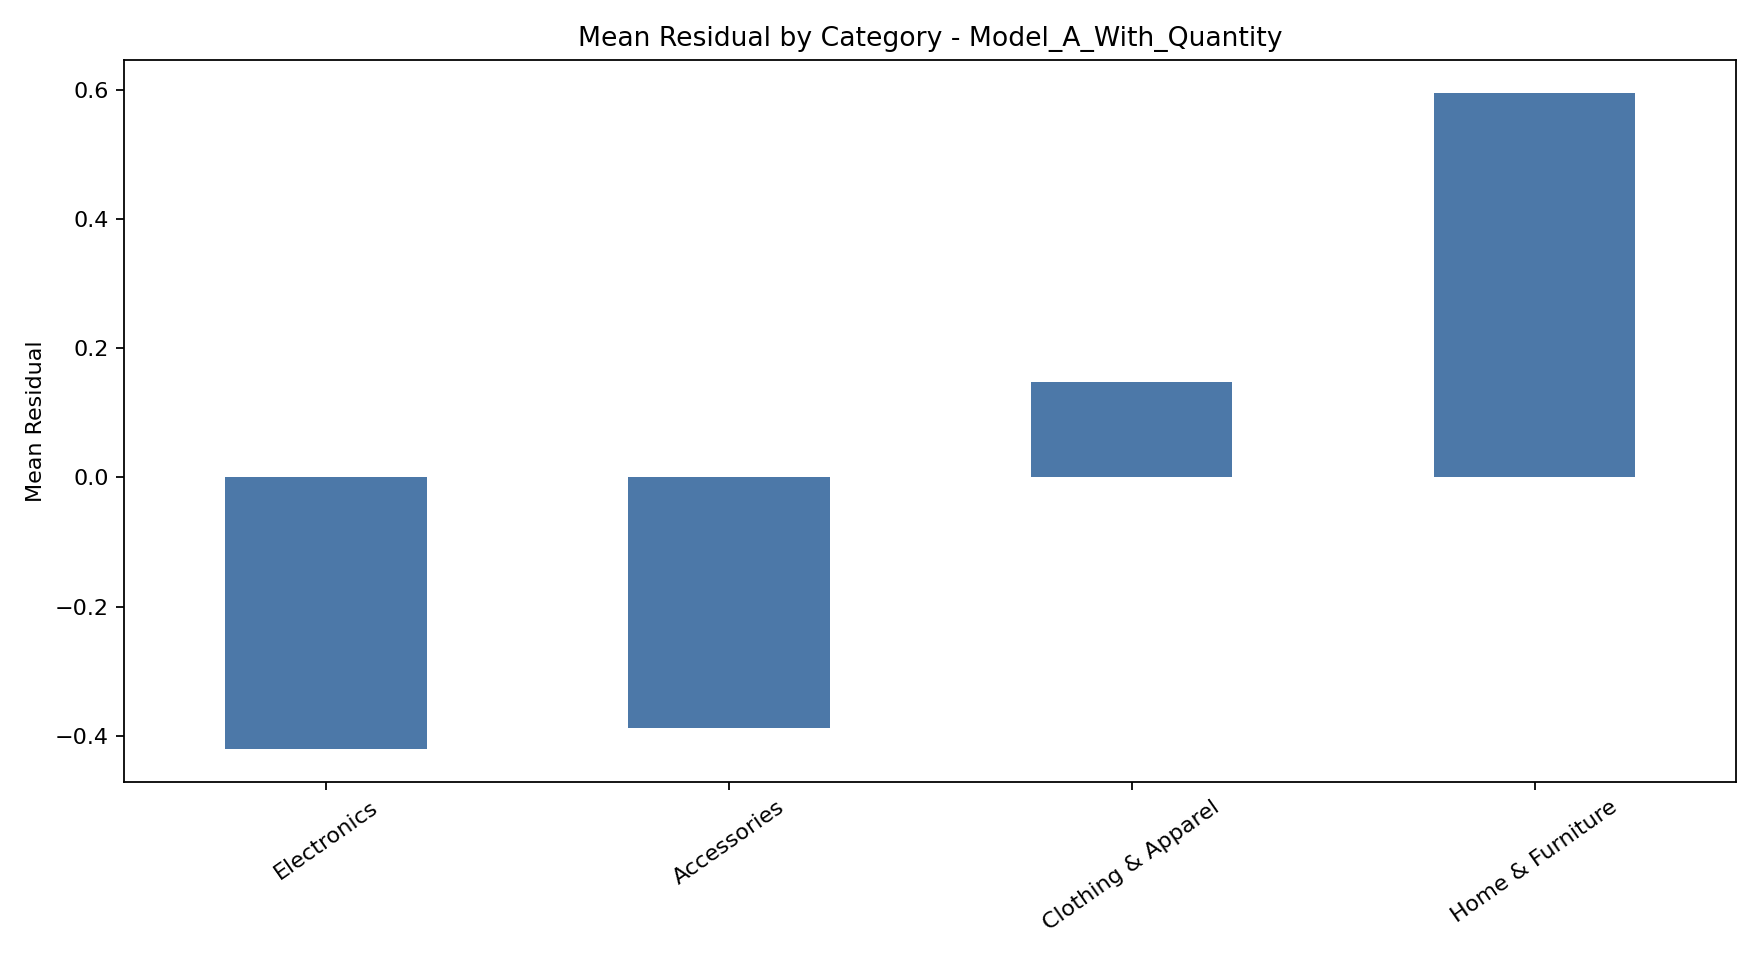
\includegraphics[width=\textwidth]{figures/lab02/residual_by_category_model_a_with_quantity.png}
  \caption{Residuals by category: Model A}
\end{figure}
\begin{figure}[H]
  \centering
  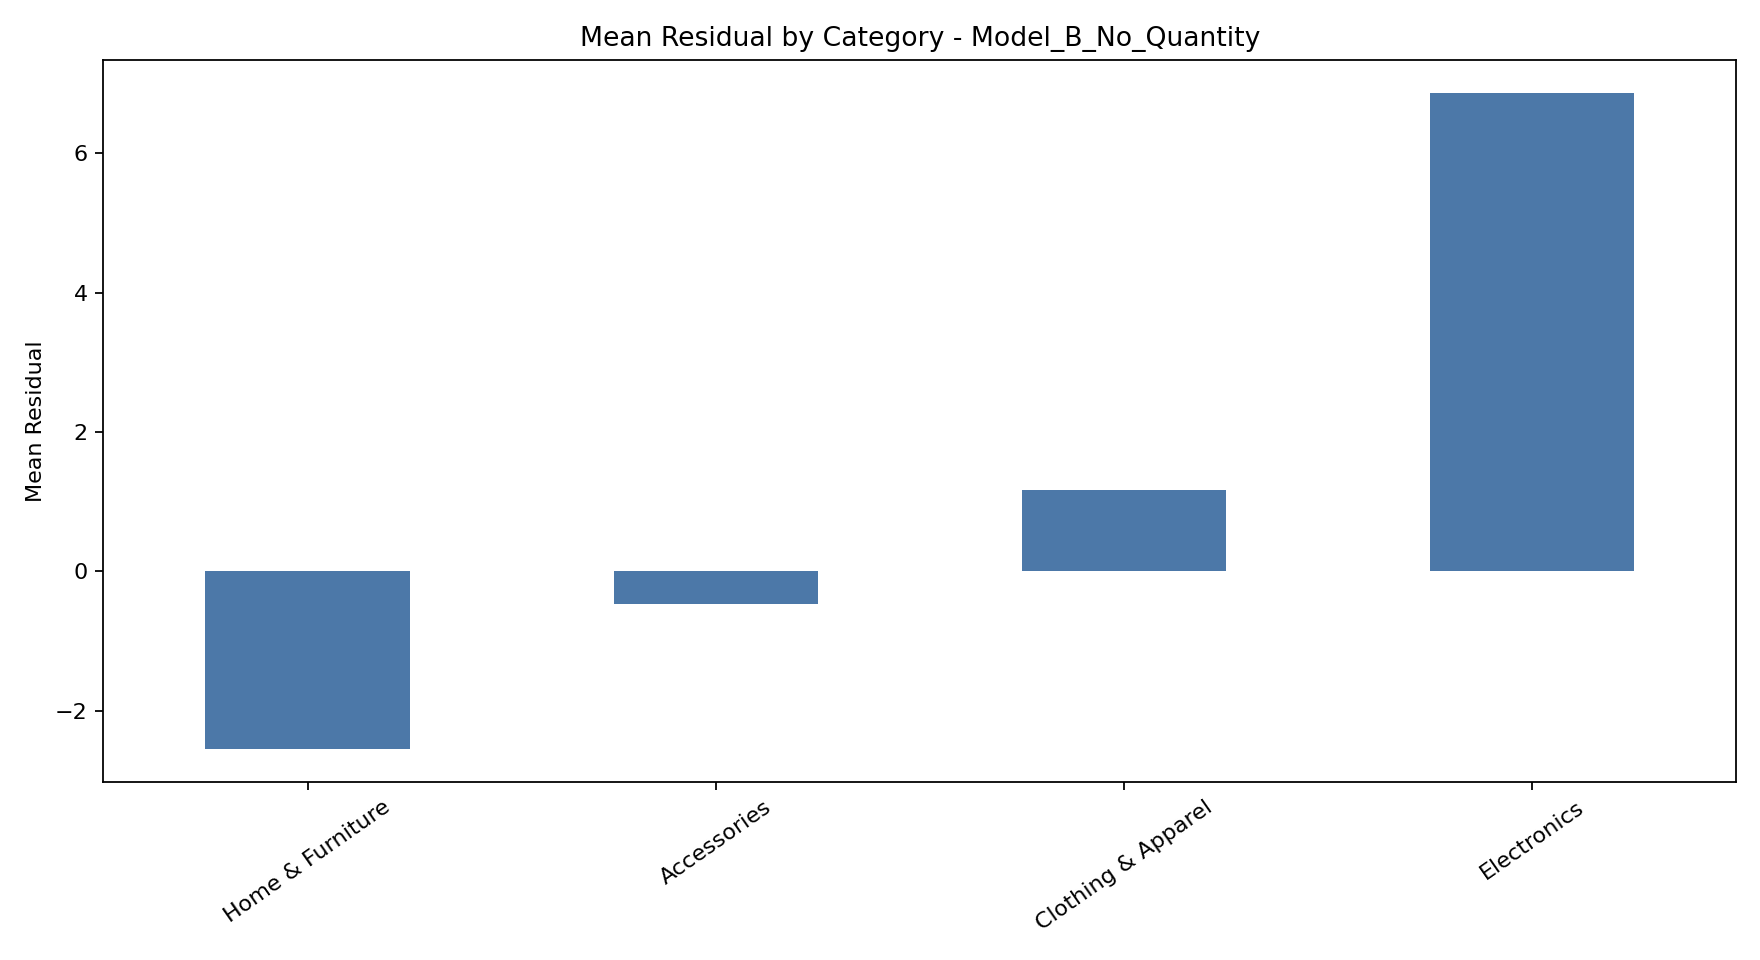
\includegraphics[width=\textwidth]{figures/lab02/residual_by_category_model_b_no_quantity.png}
  \caption{Residuals by category: Model B}
\end{figure}
\end{figure}

\begin{figure}[H]\centering
\begin{figure}[H]
  \centering
  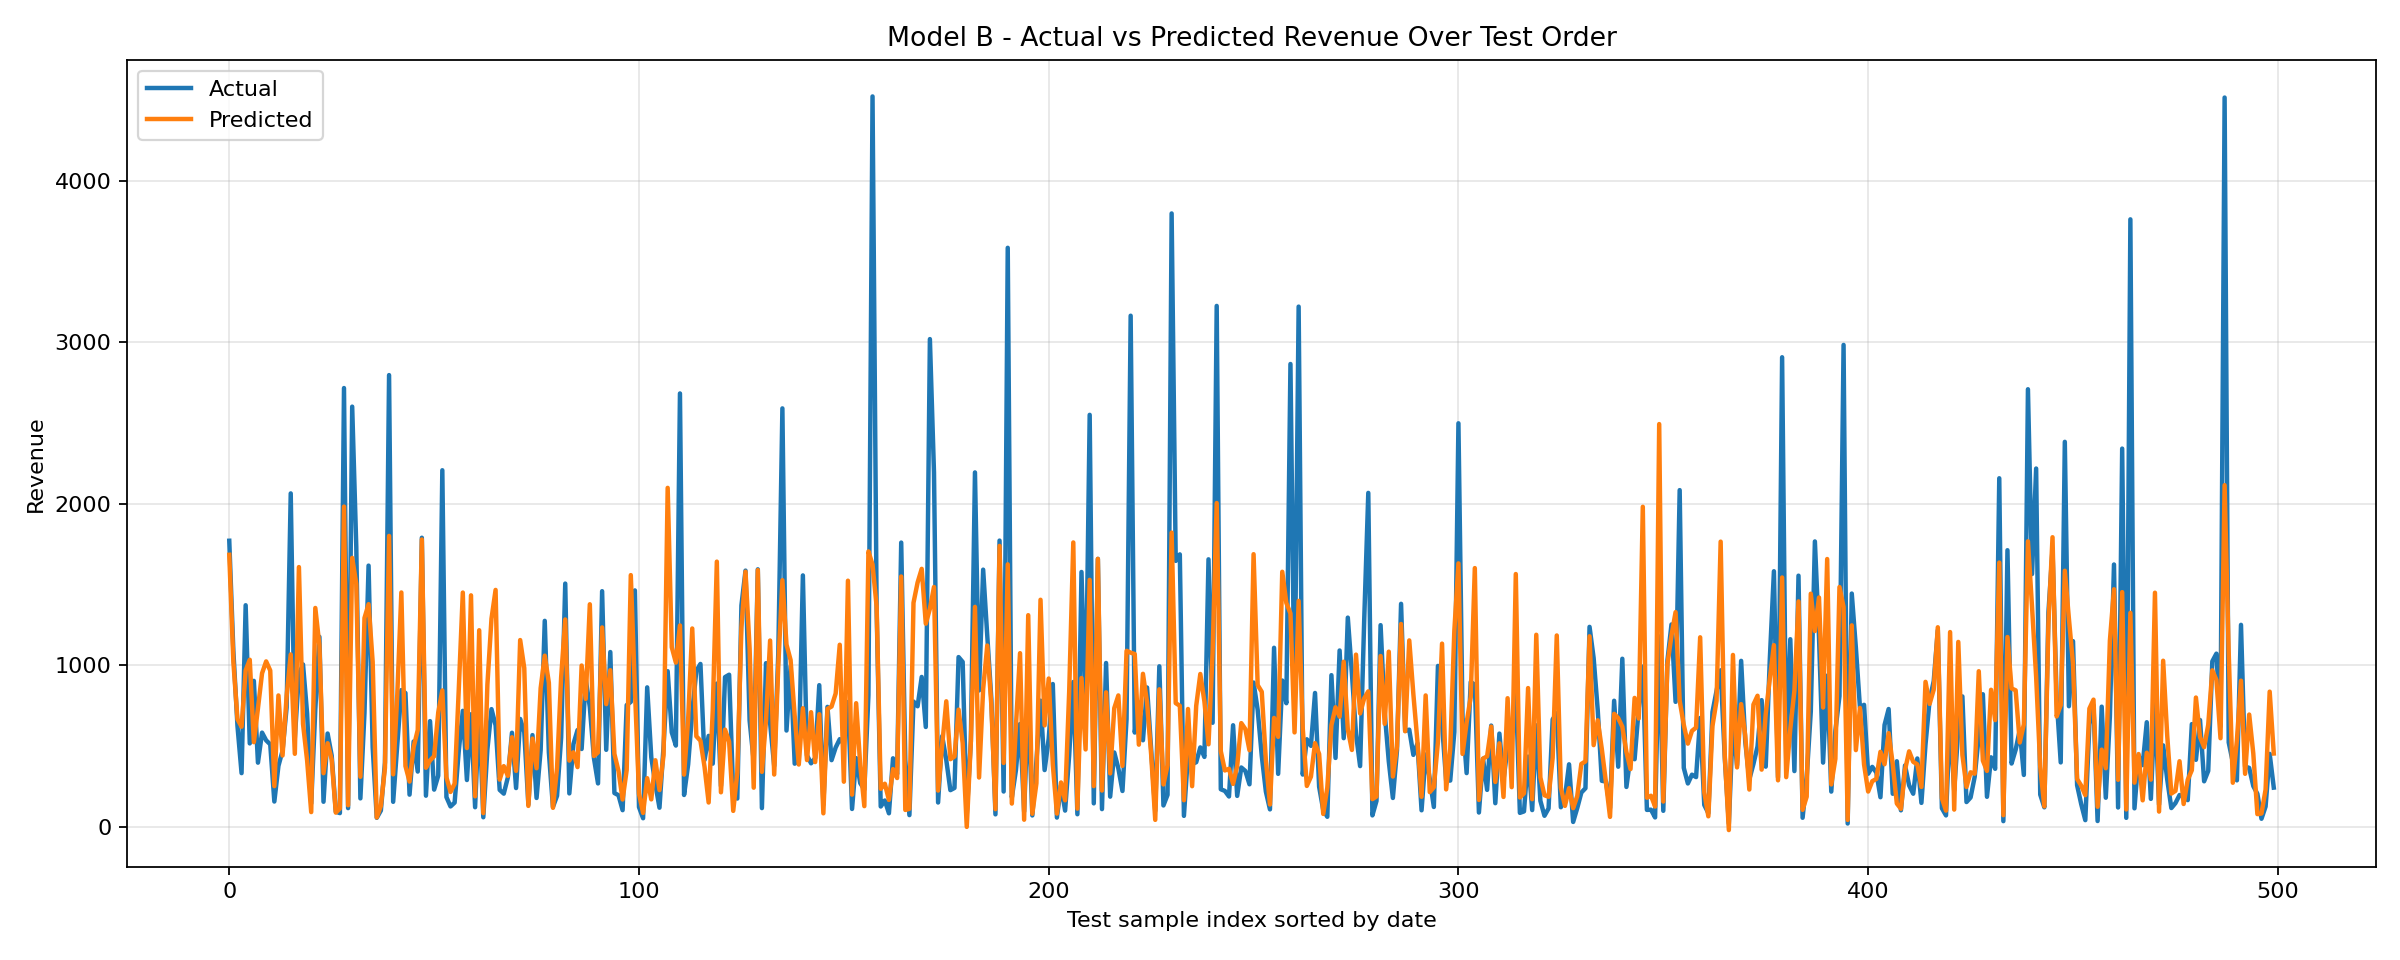
\includegraphics[width=\textwidth]{figures/lab02/notebook_model_b_actual_vs_predicted_line.png}
  \caption{Actual vs. predicted line plot}
\end{figure}
\begin{figure}[H]
  \centering
  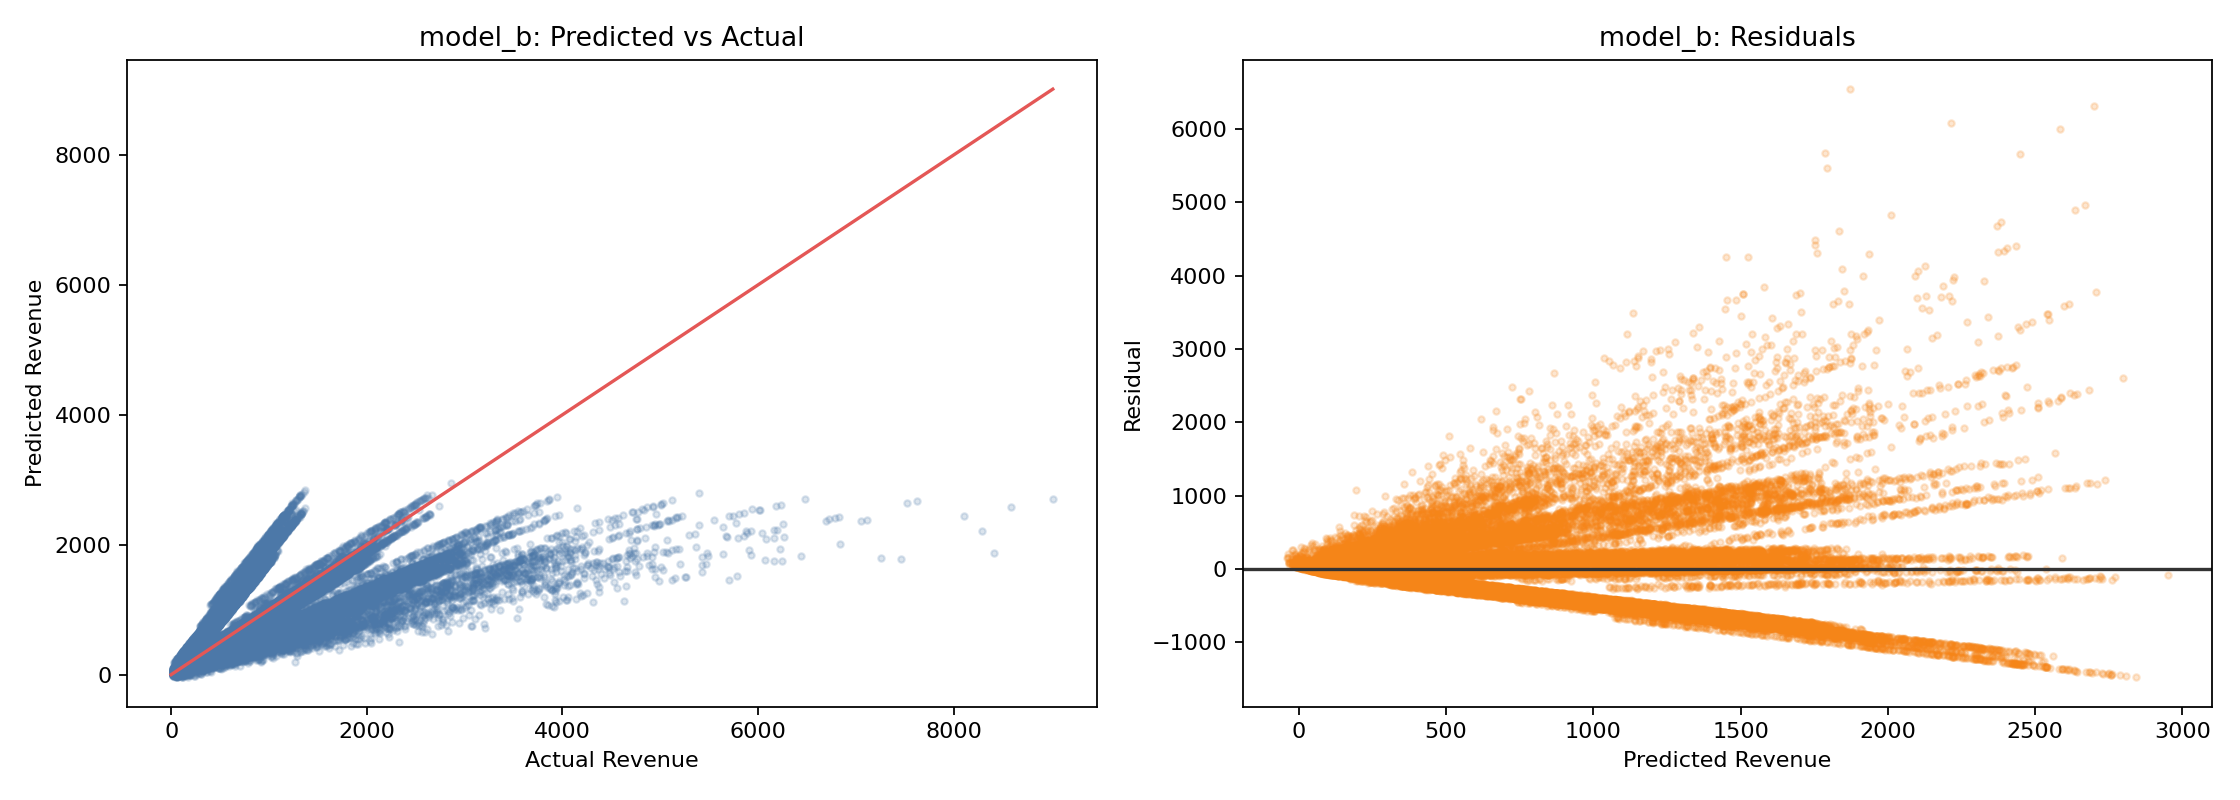
\includegraphics[width=\textwidth]{figures/lab02/notebook_model_b_prediction_plots.png}
  \caption{Prediction analysis dashboard}
\end{figure}
\end{figure}

\begin{figure}[H]\centering
\begin{figure}[H]
  \centering
  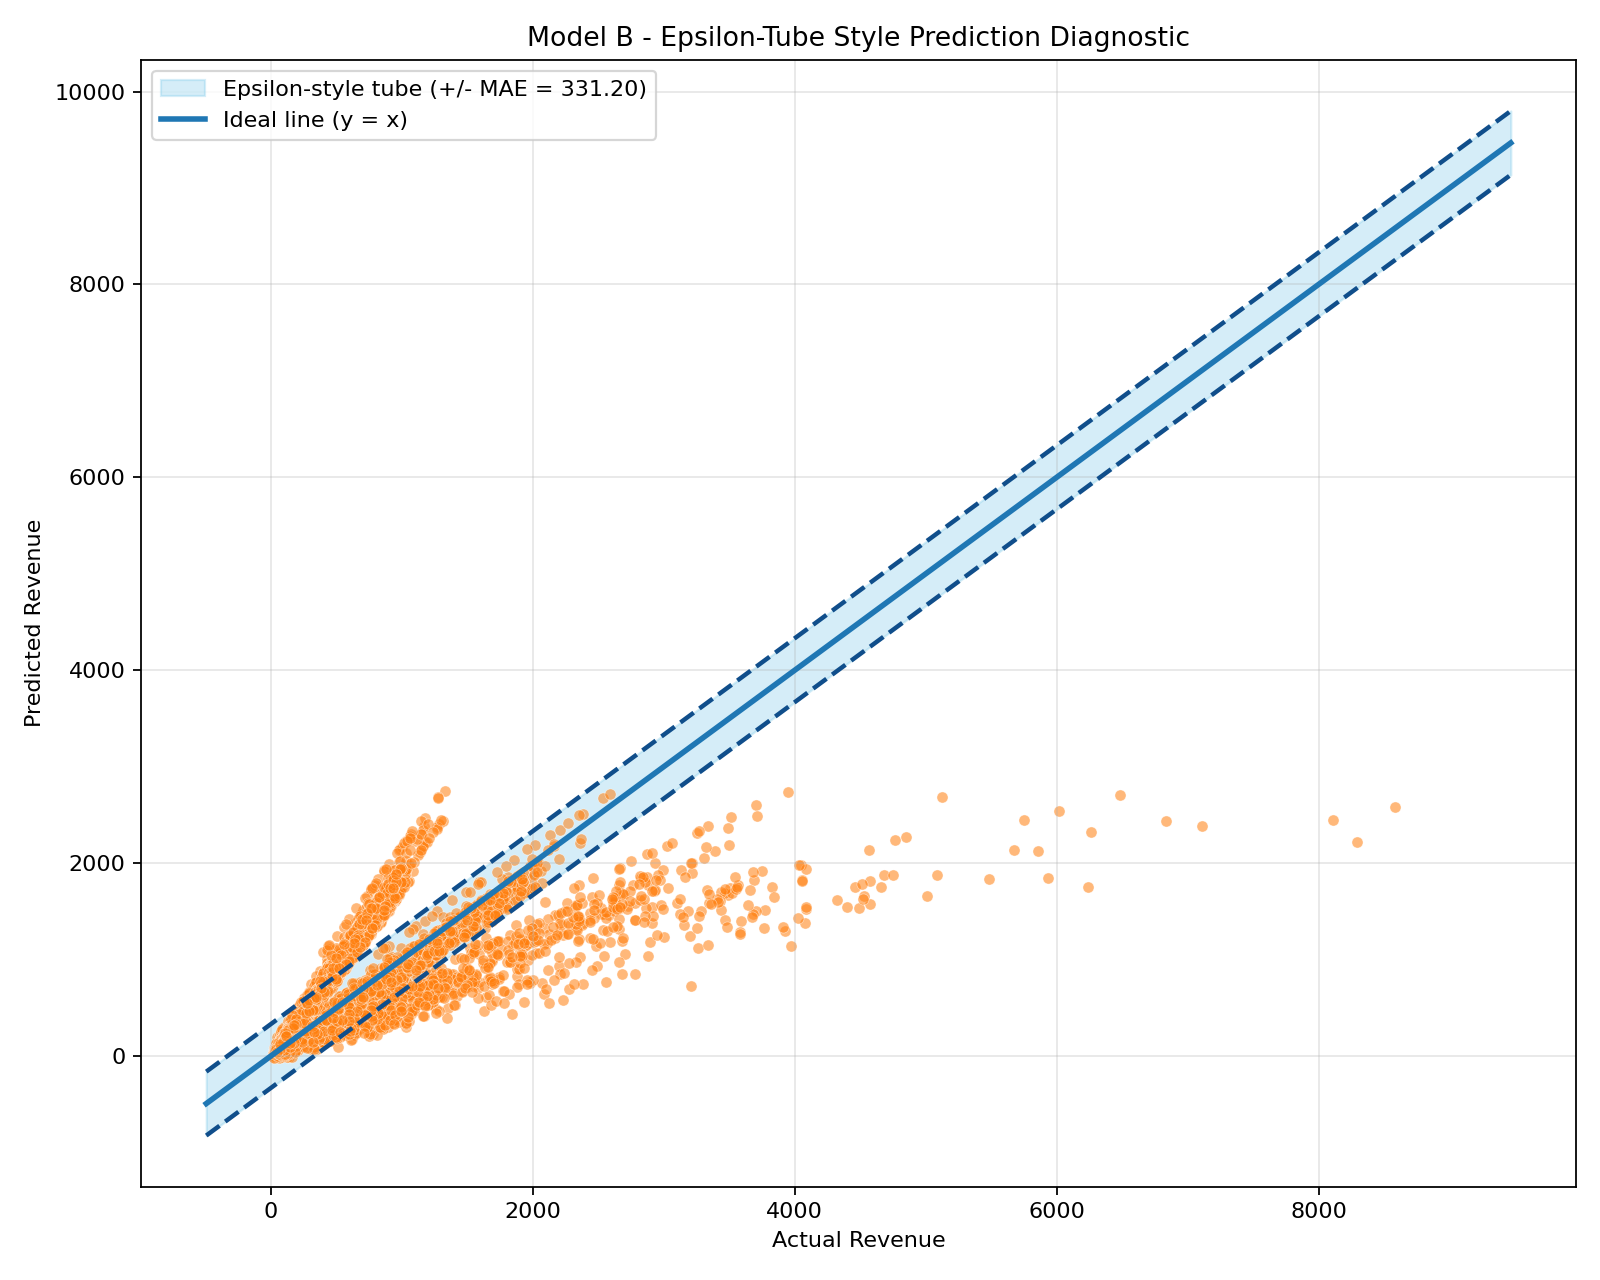
\includegraphics[width=\textwidth]{figures/lab02/notebook_model_b_epsilon_tube_style.png}
  \caption{Epsilon-tube style plot}
\end{figure}
\begin{figure}[H]
  \centering
  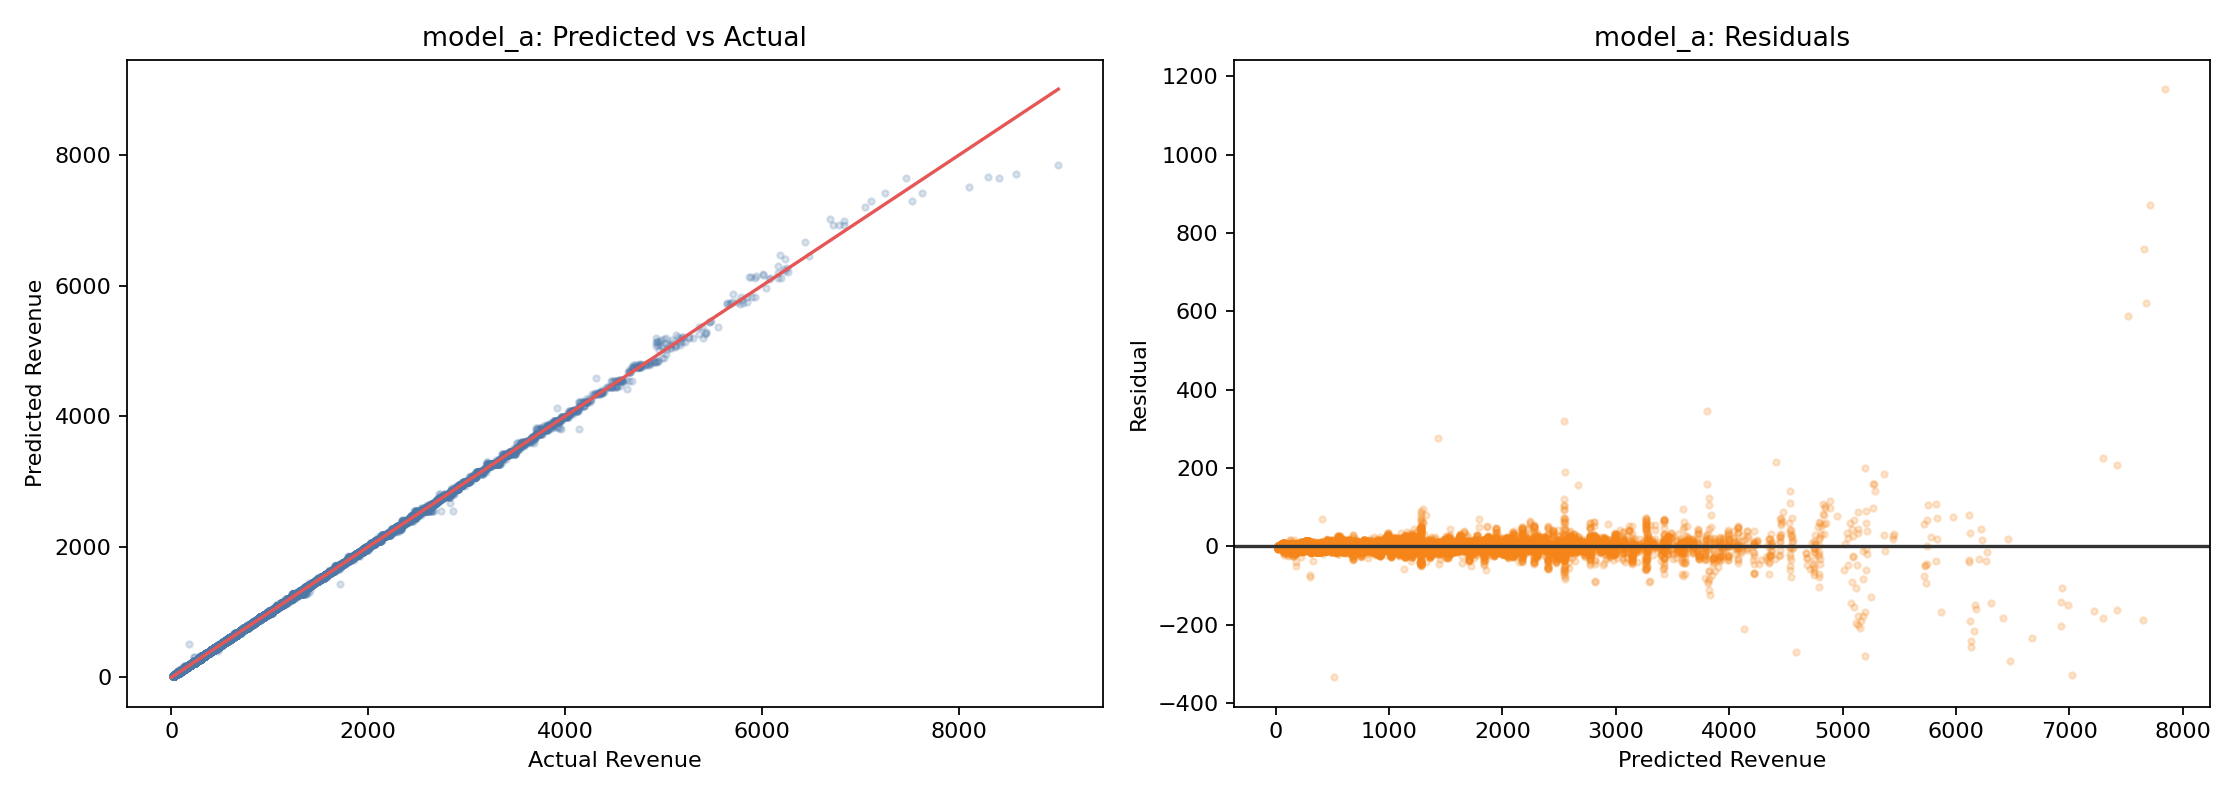
\includegraphics[width=\textwidth]{figures/lab02/notebook_model_a_prediction_plots.png}
  \caption{Model A prediction plots}
\end{figure}
\end{figure}

\begin{figure}[H]\centering
\begin{figure}[H]
  \centering
  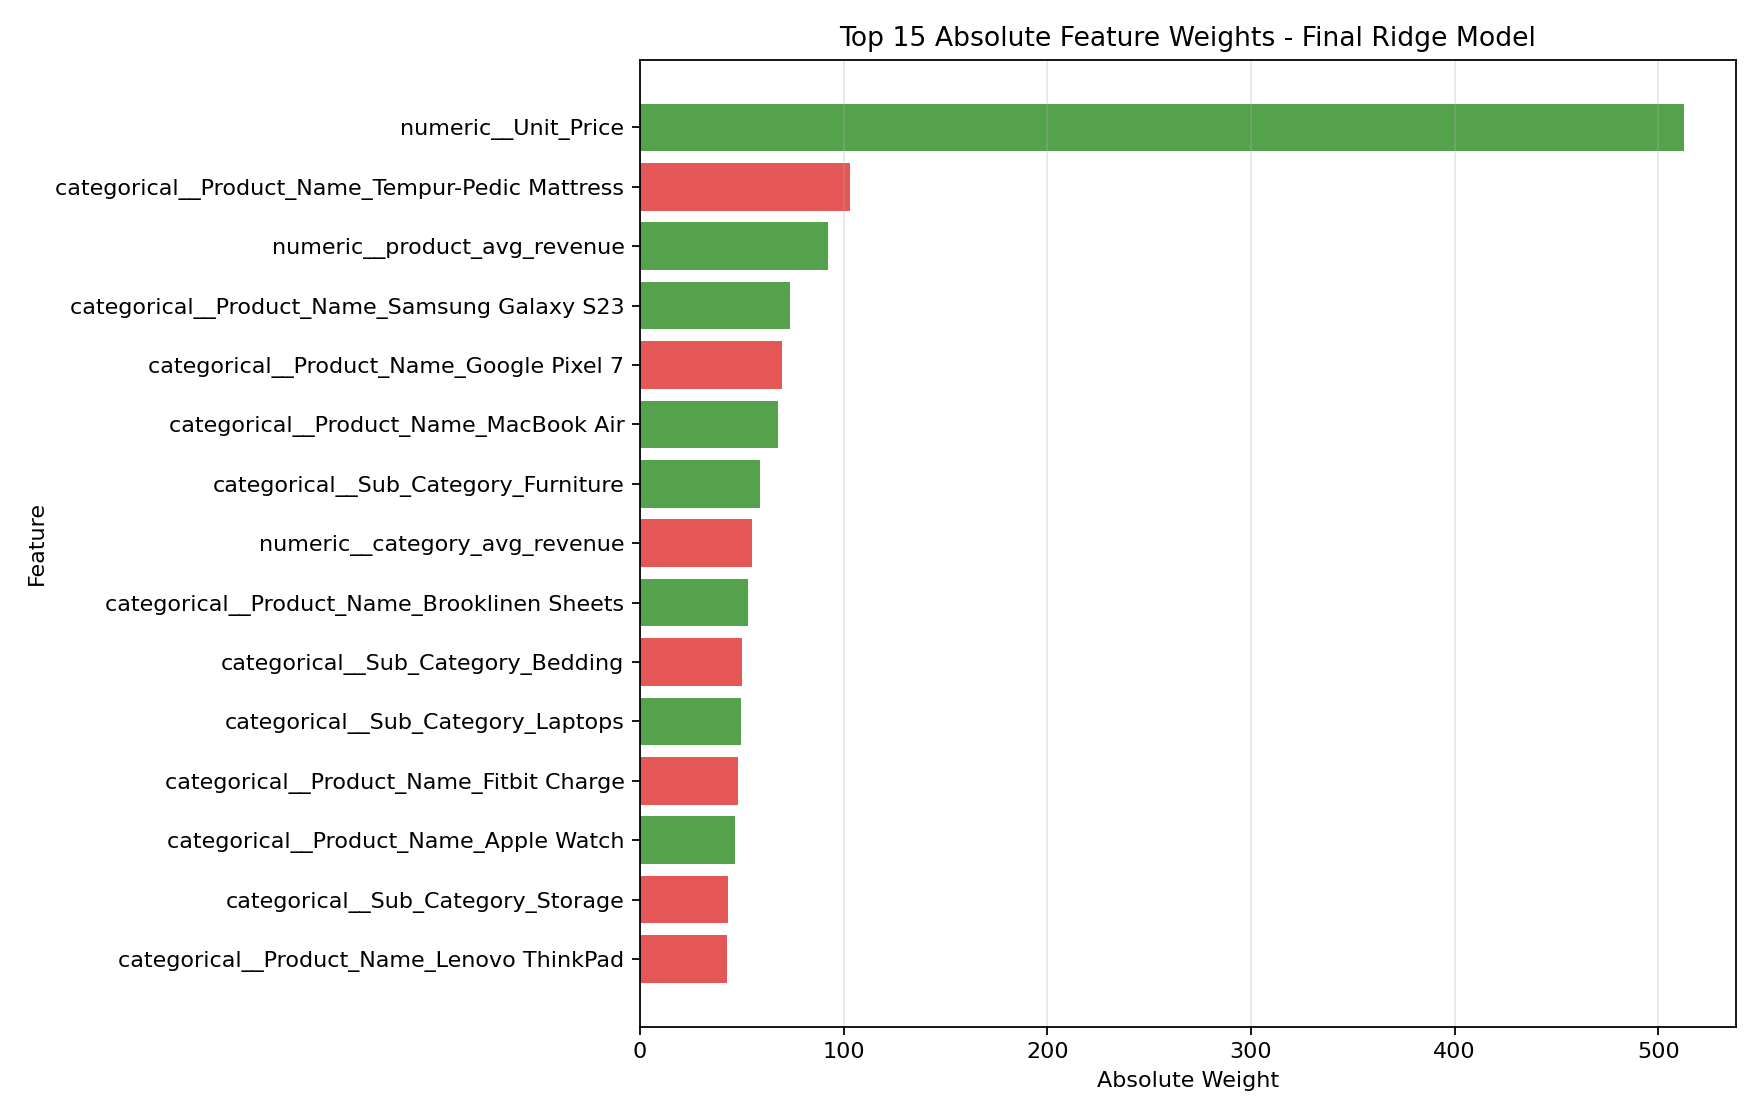
\includegraphics[width=\textwidth]{figures/lab02/notebook_final_ridge_feature_weights.png}
  \caption{Ridge feature weights}
\end{figure}
\begin{figure}[H]
  \centering
  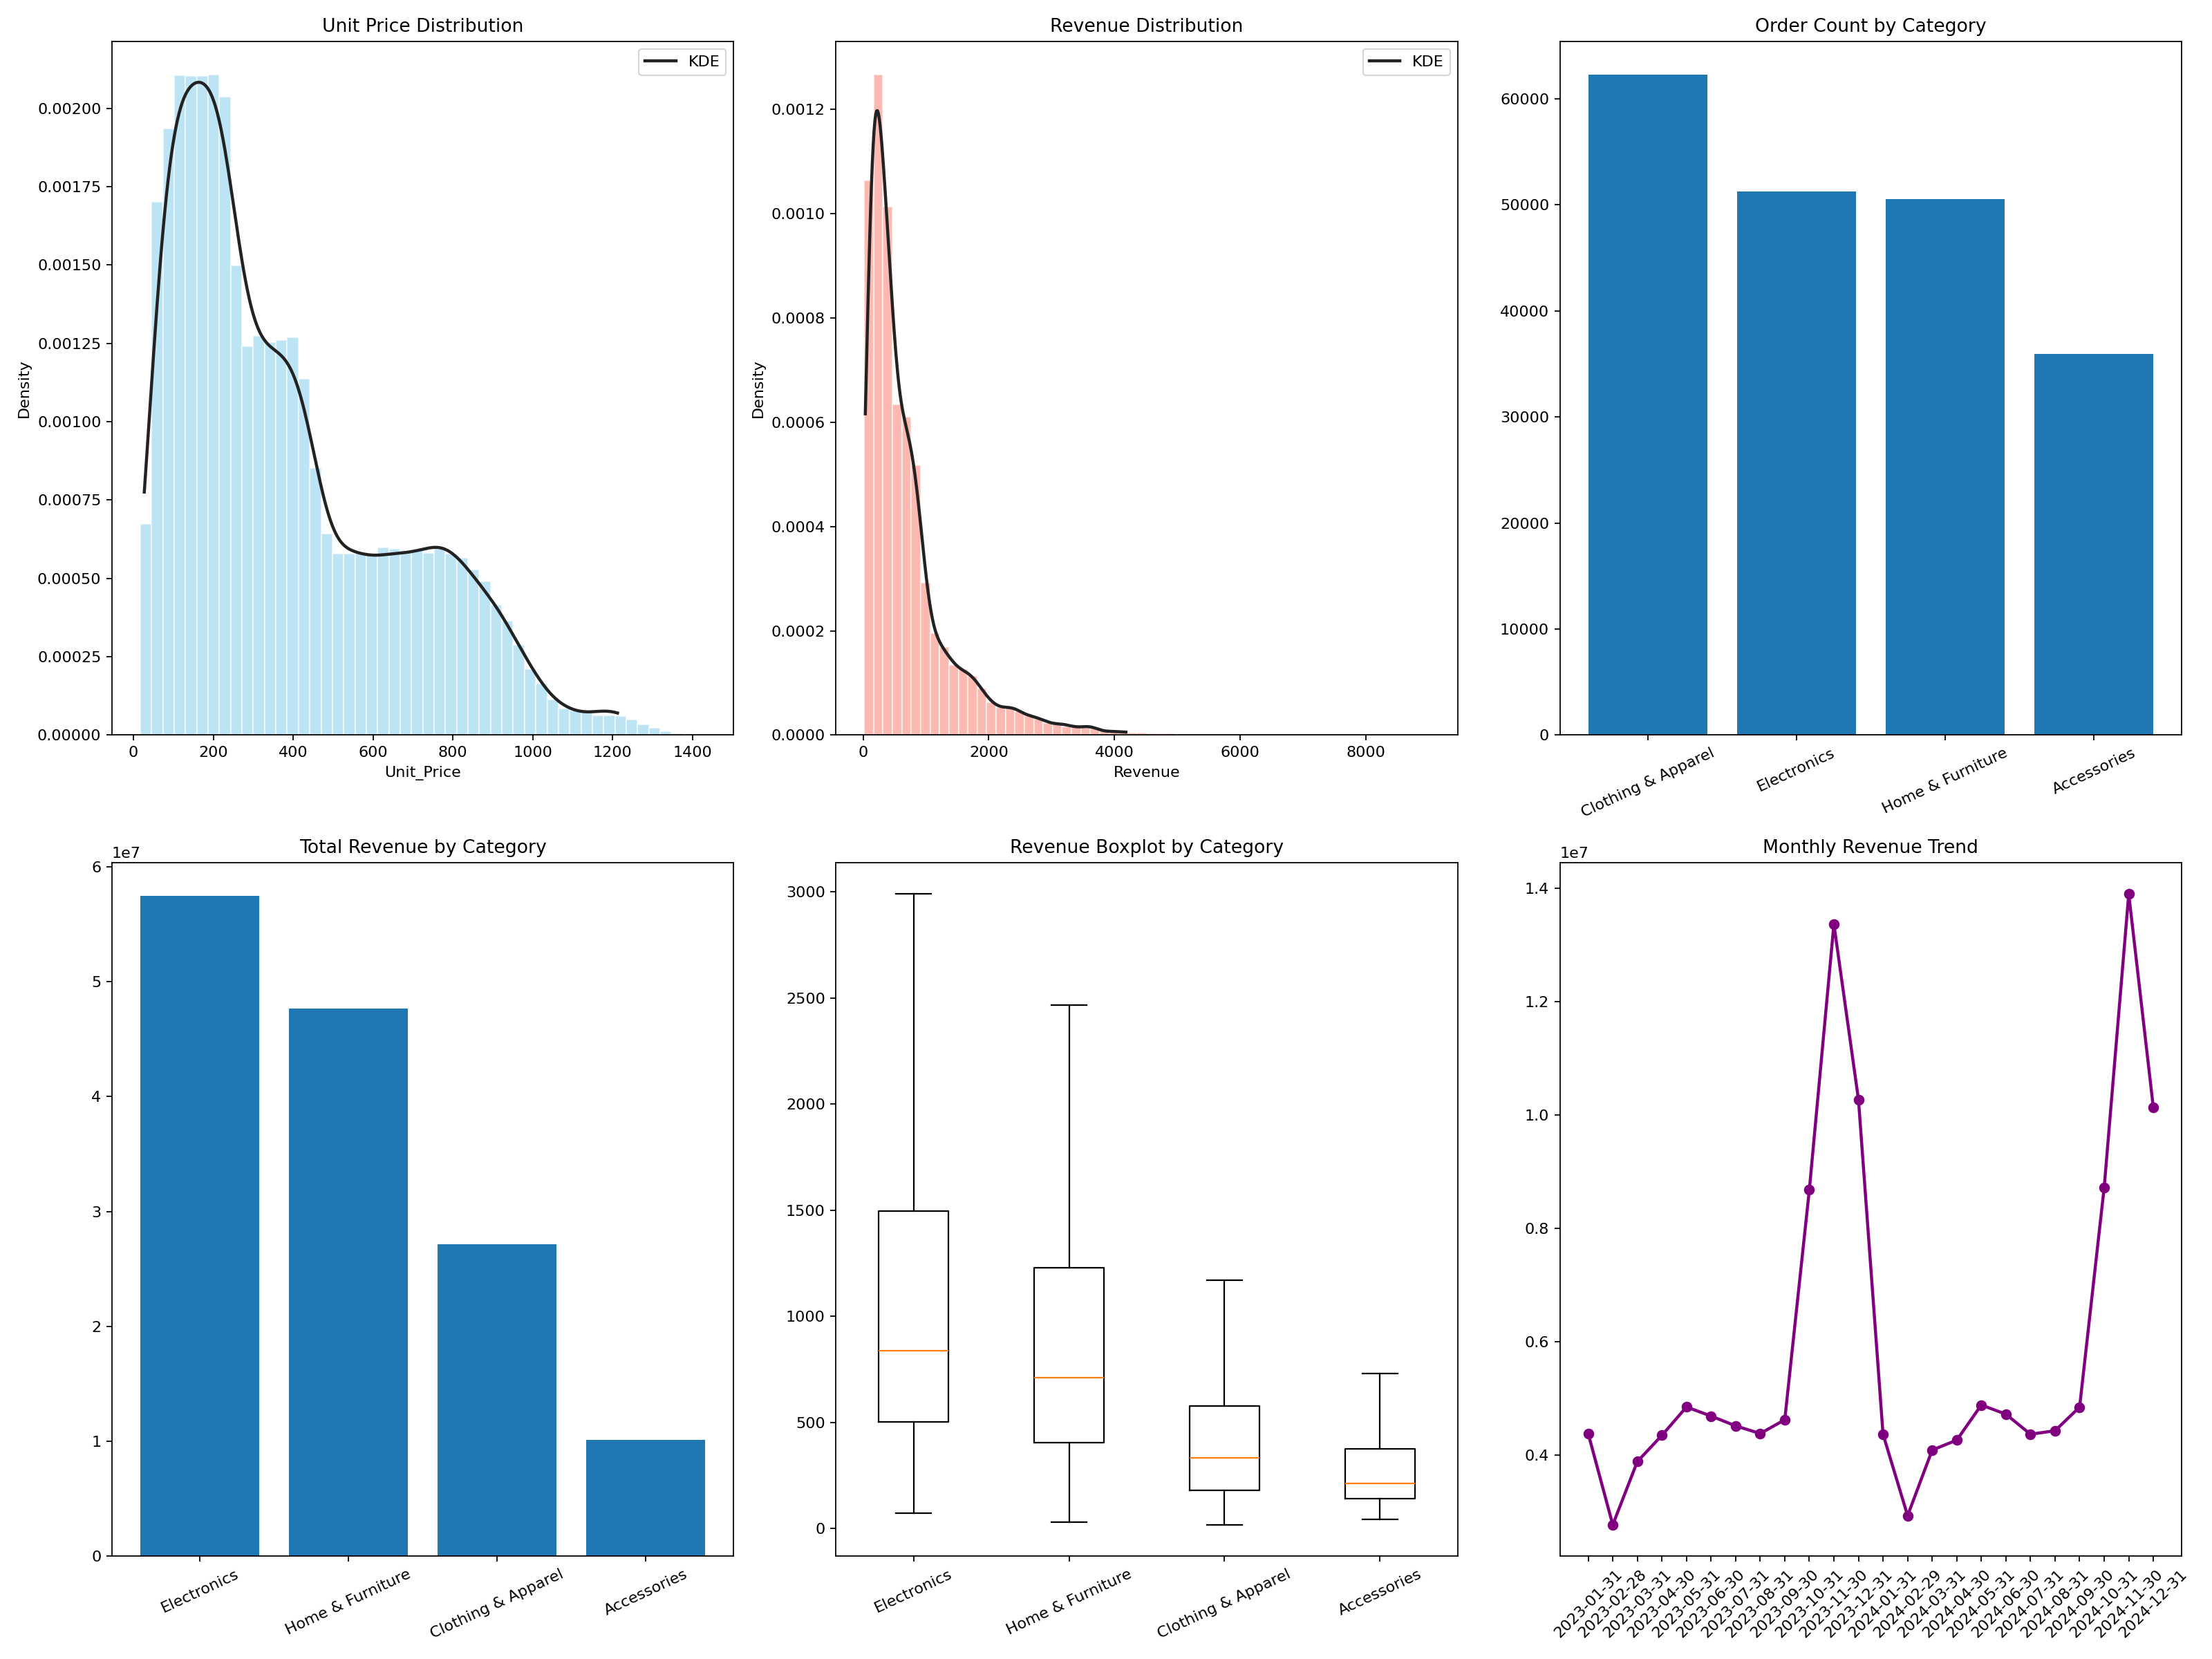
\includegraphics[width=\textwidth]{figures/lab02/notebook_full_eda_dashboard_like_sample.png}
  \caption{Full EDA dashboard}
\end{figure}
\end{figure}

\begin{figure}[H]\centering
\begin{figure}[H]
  \centering
  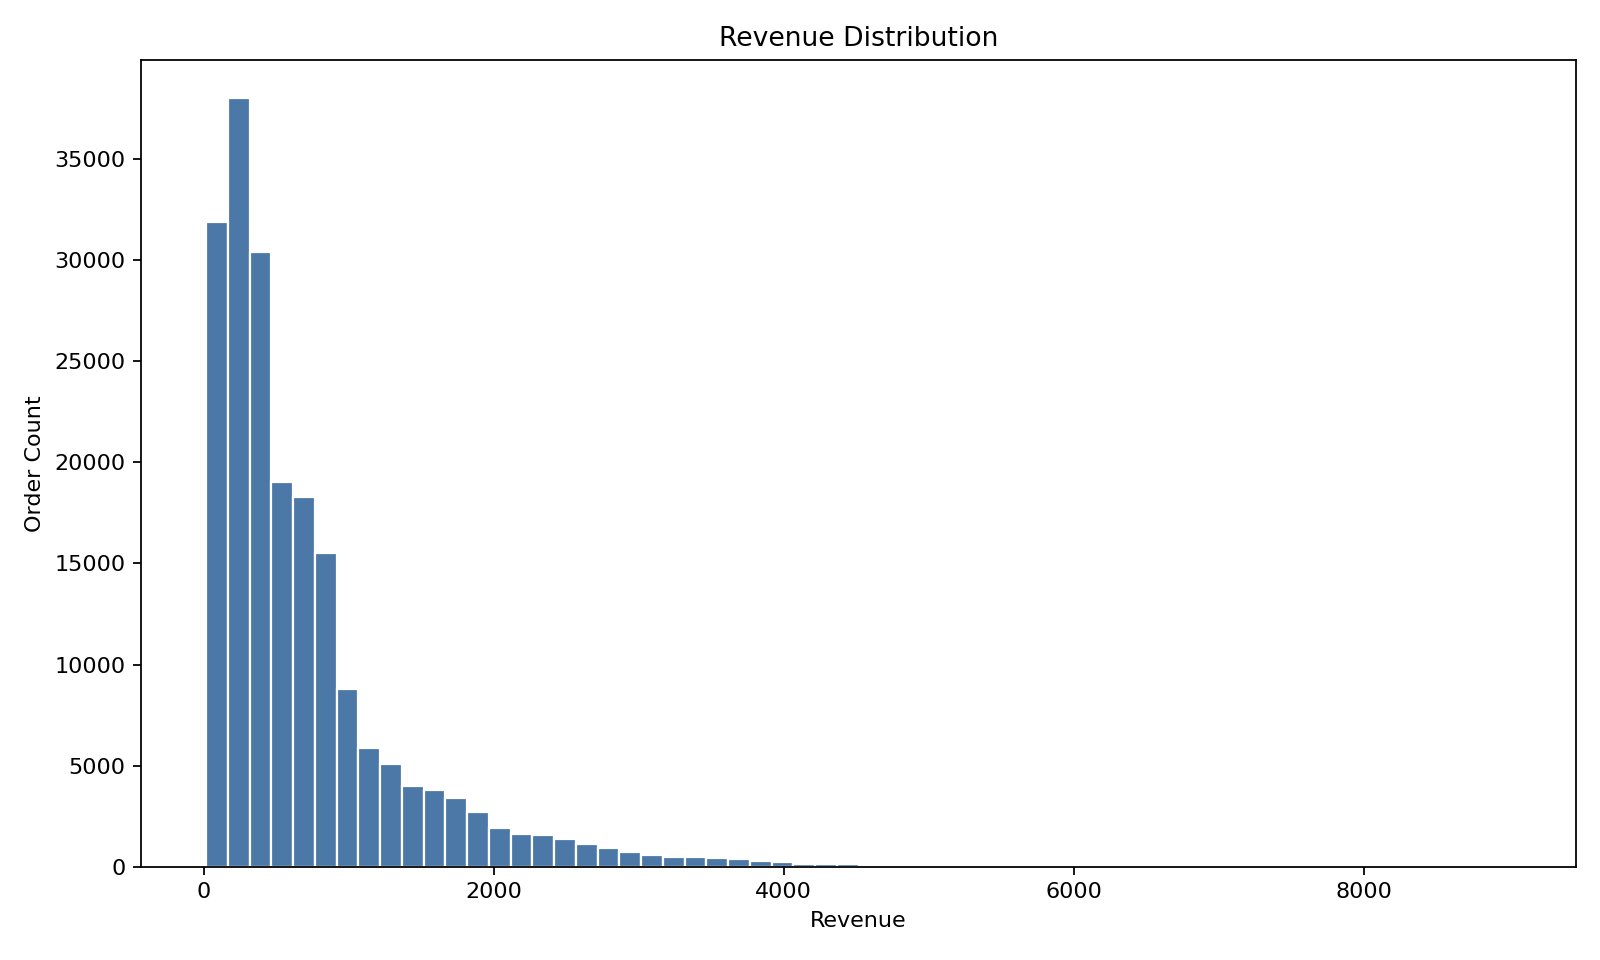
\includegraphics[width=\textwidth]{figures/lab02/revenue_distribution.png}
  \caption{Revenue distribution histogram}
\end{figure}
\begin{figure}[H]
  \centering
  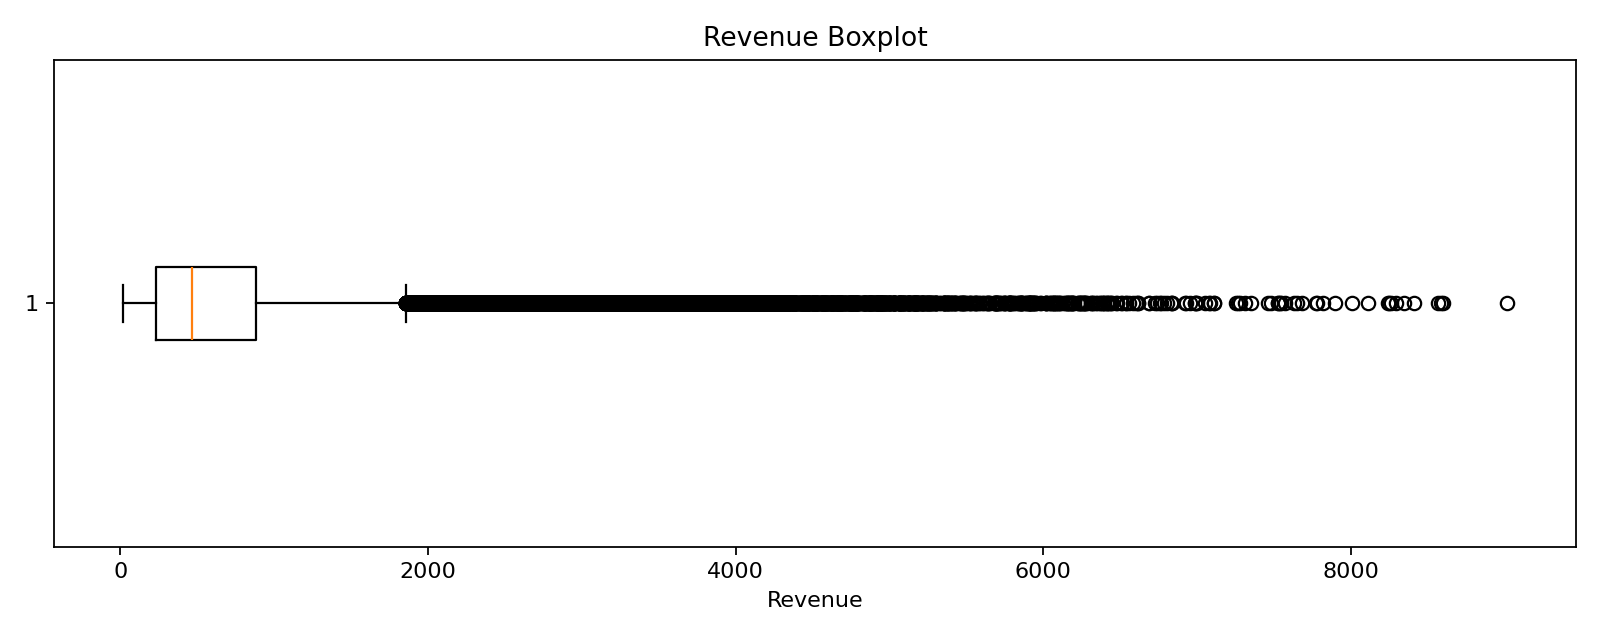
\includegraphics[width=\textwidth]{figures/lab02/revenue_boxplot.png}
  \caption{Revenue boxplot}
\end{figure}\
\vspace{4pt}
\begin{figure}[H]
  \centering
  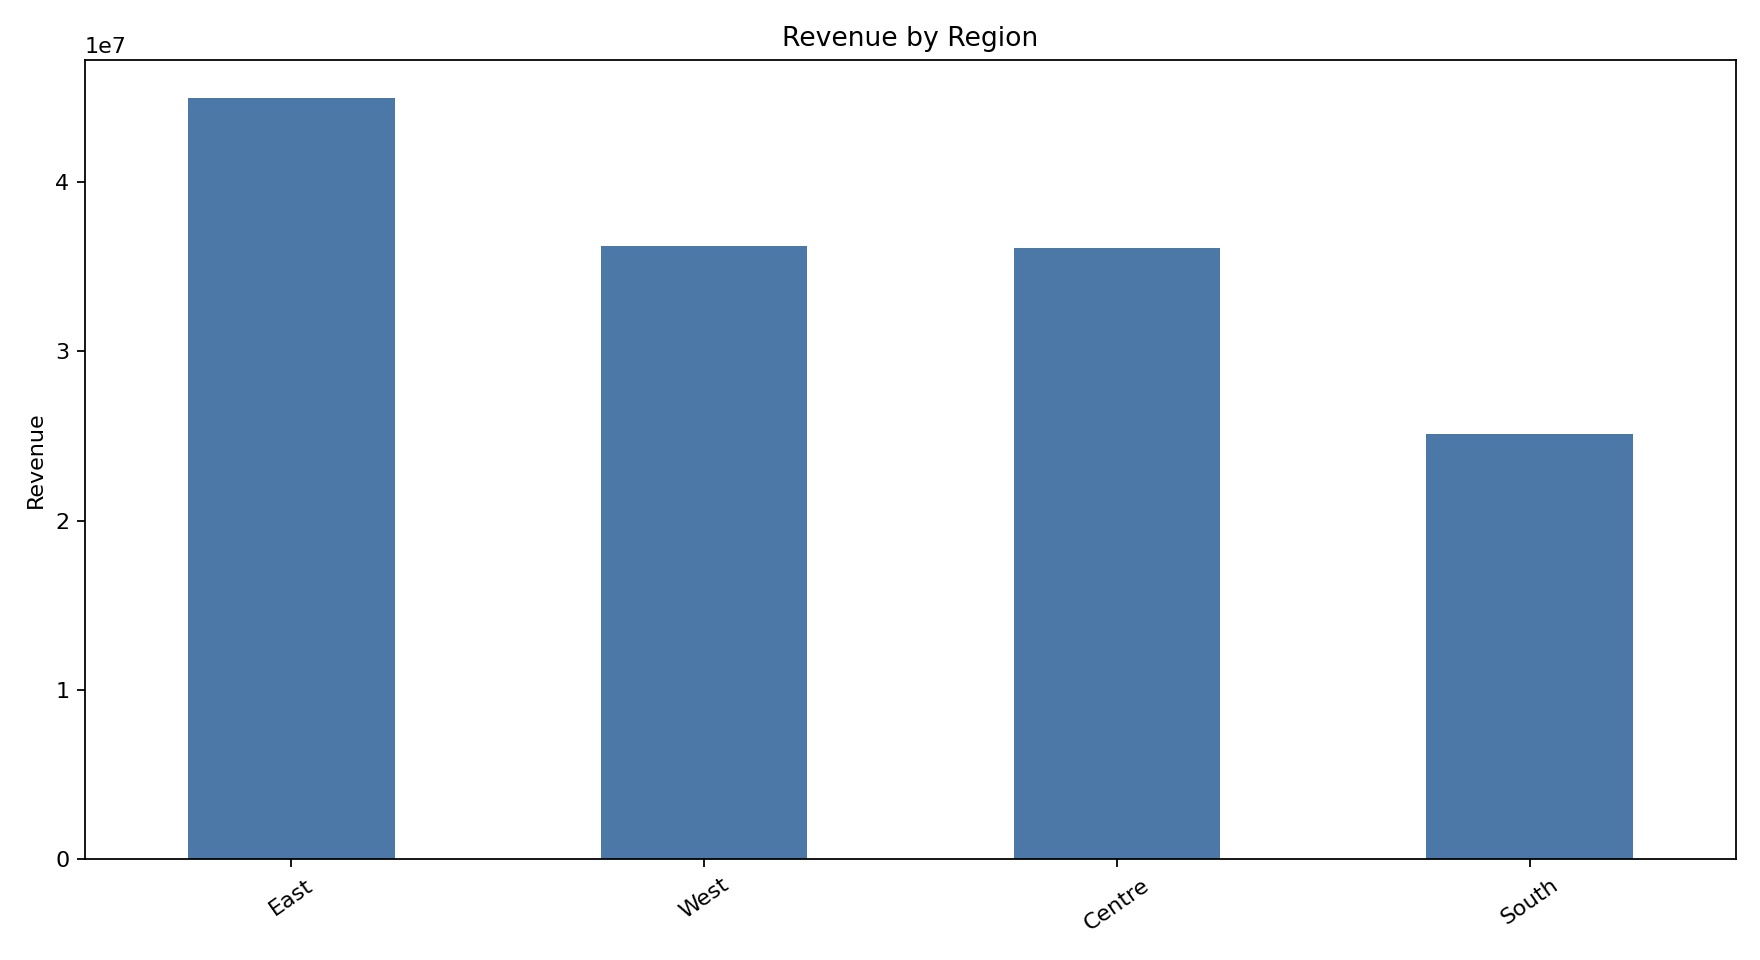
\includegraphics[width=\textwidth]{figures/lab02/revenue_by_region.png}
  \caption{Revenue by region}
\end{figure}
\begin{figure}[H]
  \centering
  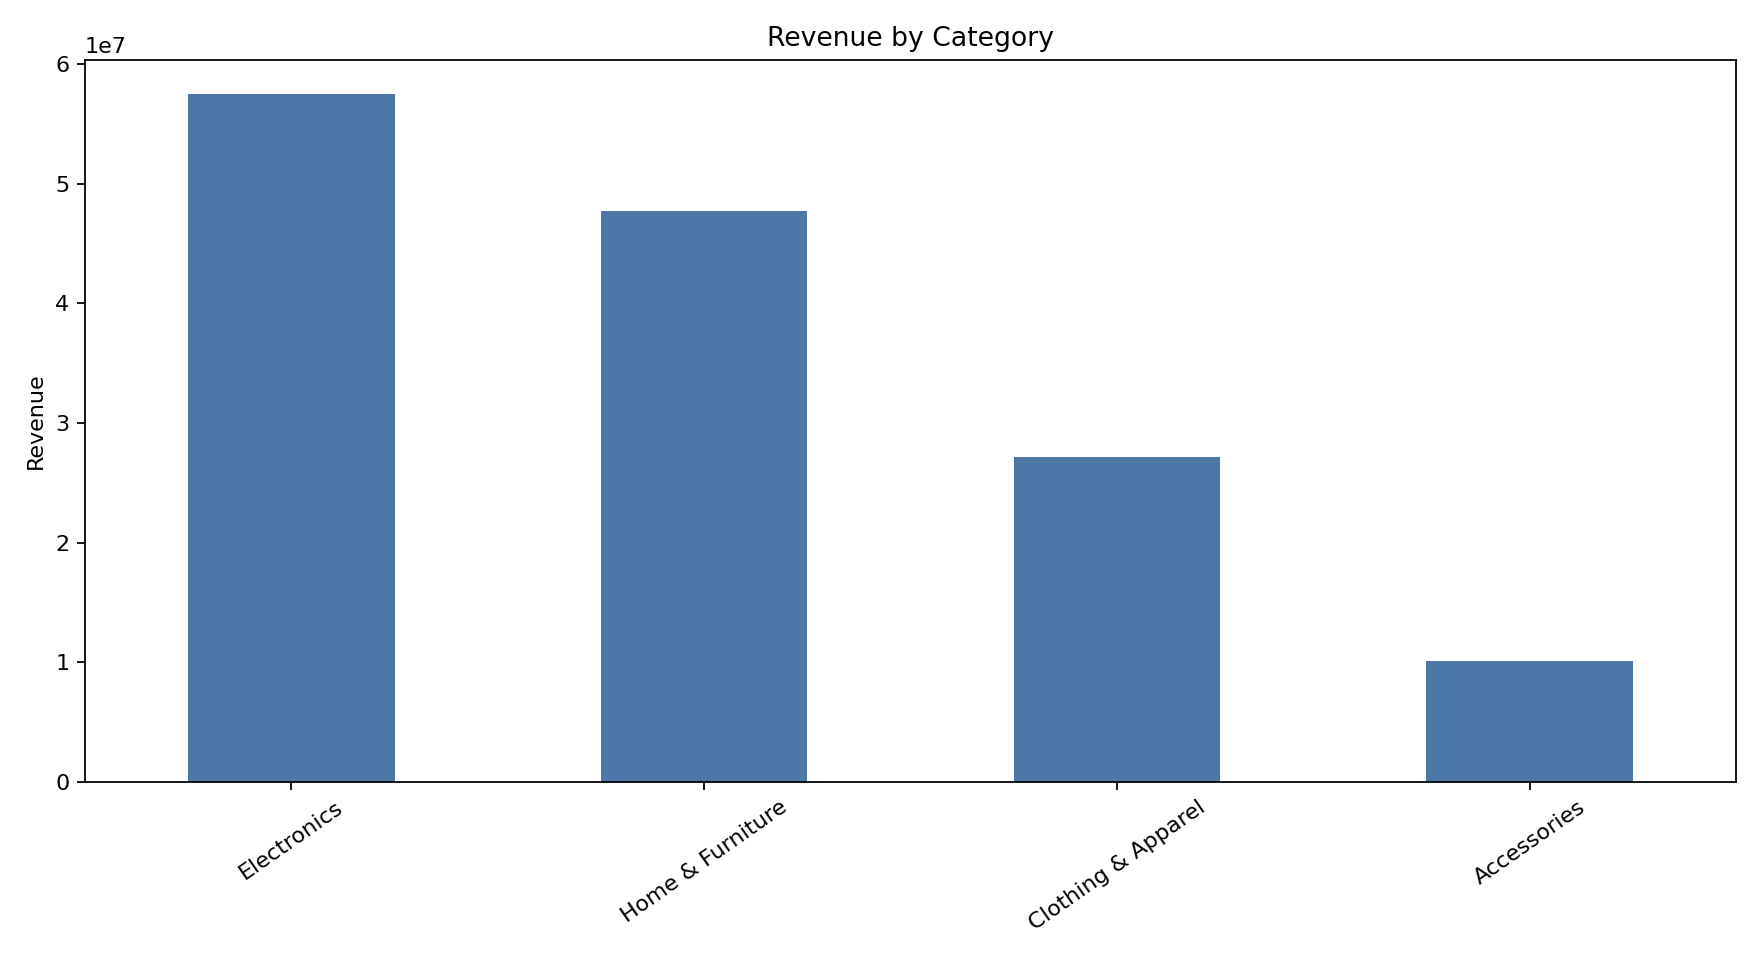
\includegraphics[width=\textwidth]{figures/lab02/revenue_by_category.png}
  \caption{Revenue by category}
\end{figure}\
\vspace{4pt}
\begin{figure}[H]
  \centering
  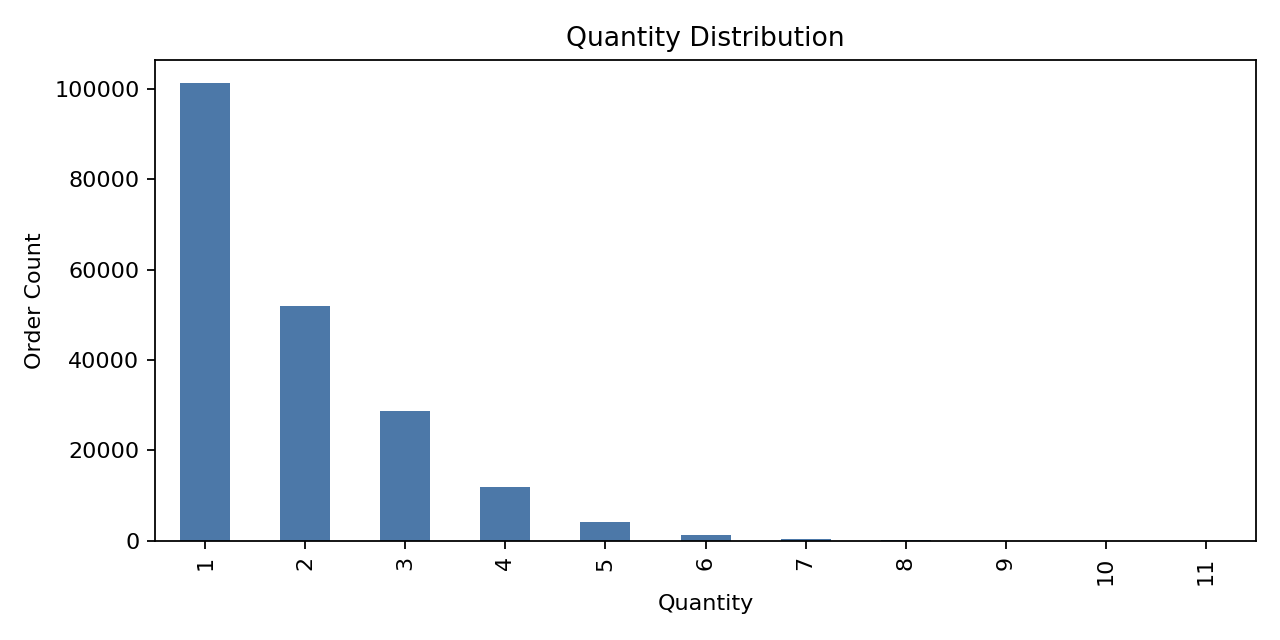
\includegraphics[width=\textwidth]{figures/lab02/quantity_distribution.png}
  \caption{Quantity distribution}
\end{figure}
\begin{figure}[H]
  \centering
  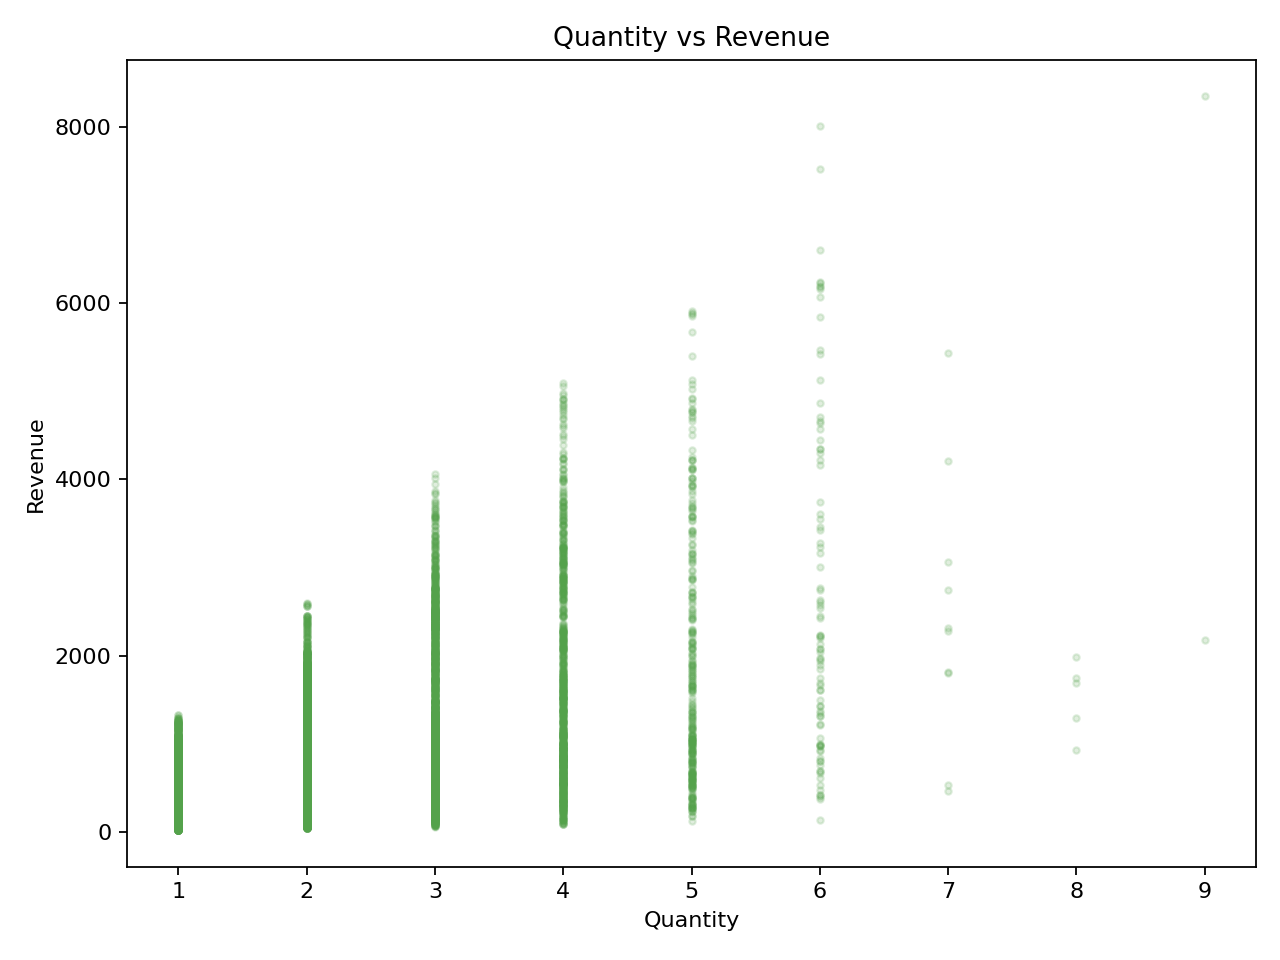
\includegraphics[width=\textwidth]{figures/lab02/quantity_vs_revenue.png}
  \caption{Quantity vs. revenue}
\end{figure}\
\vspace{4pt}
\begin{figure}[H]
  \centering
  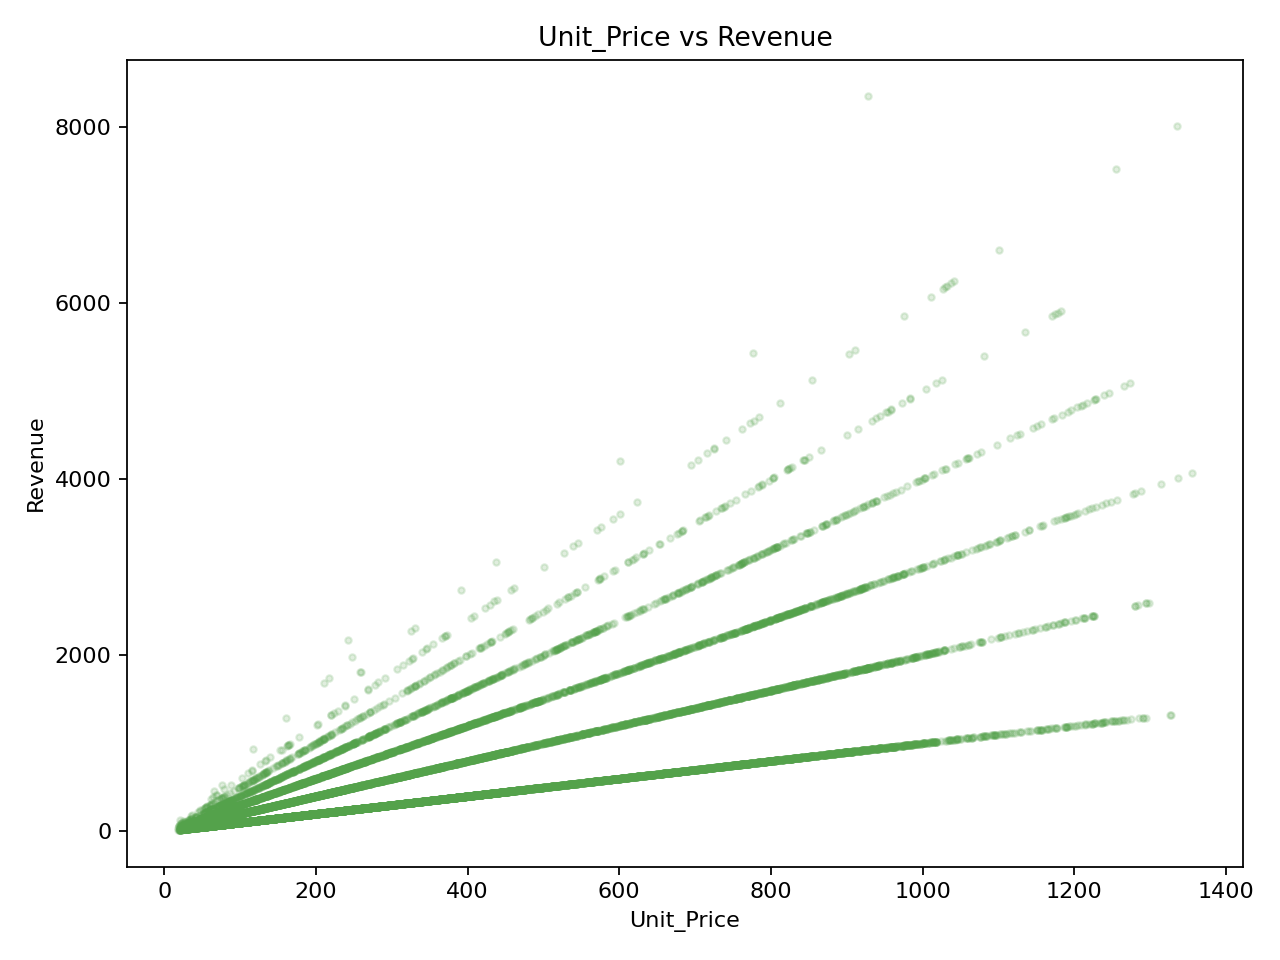
\includegraphics[width=\textwidth]{figures/lab02/unit_price_vs_revenue.png}
  \caption{Unit price vs. revenue}
\end{figure}
\begin{figure}[H]
  \centering
  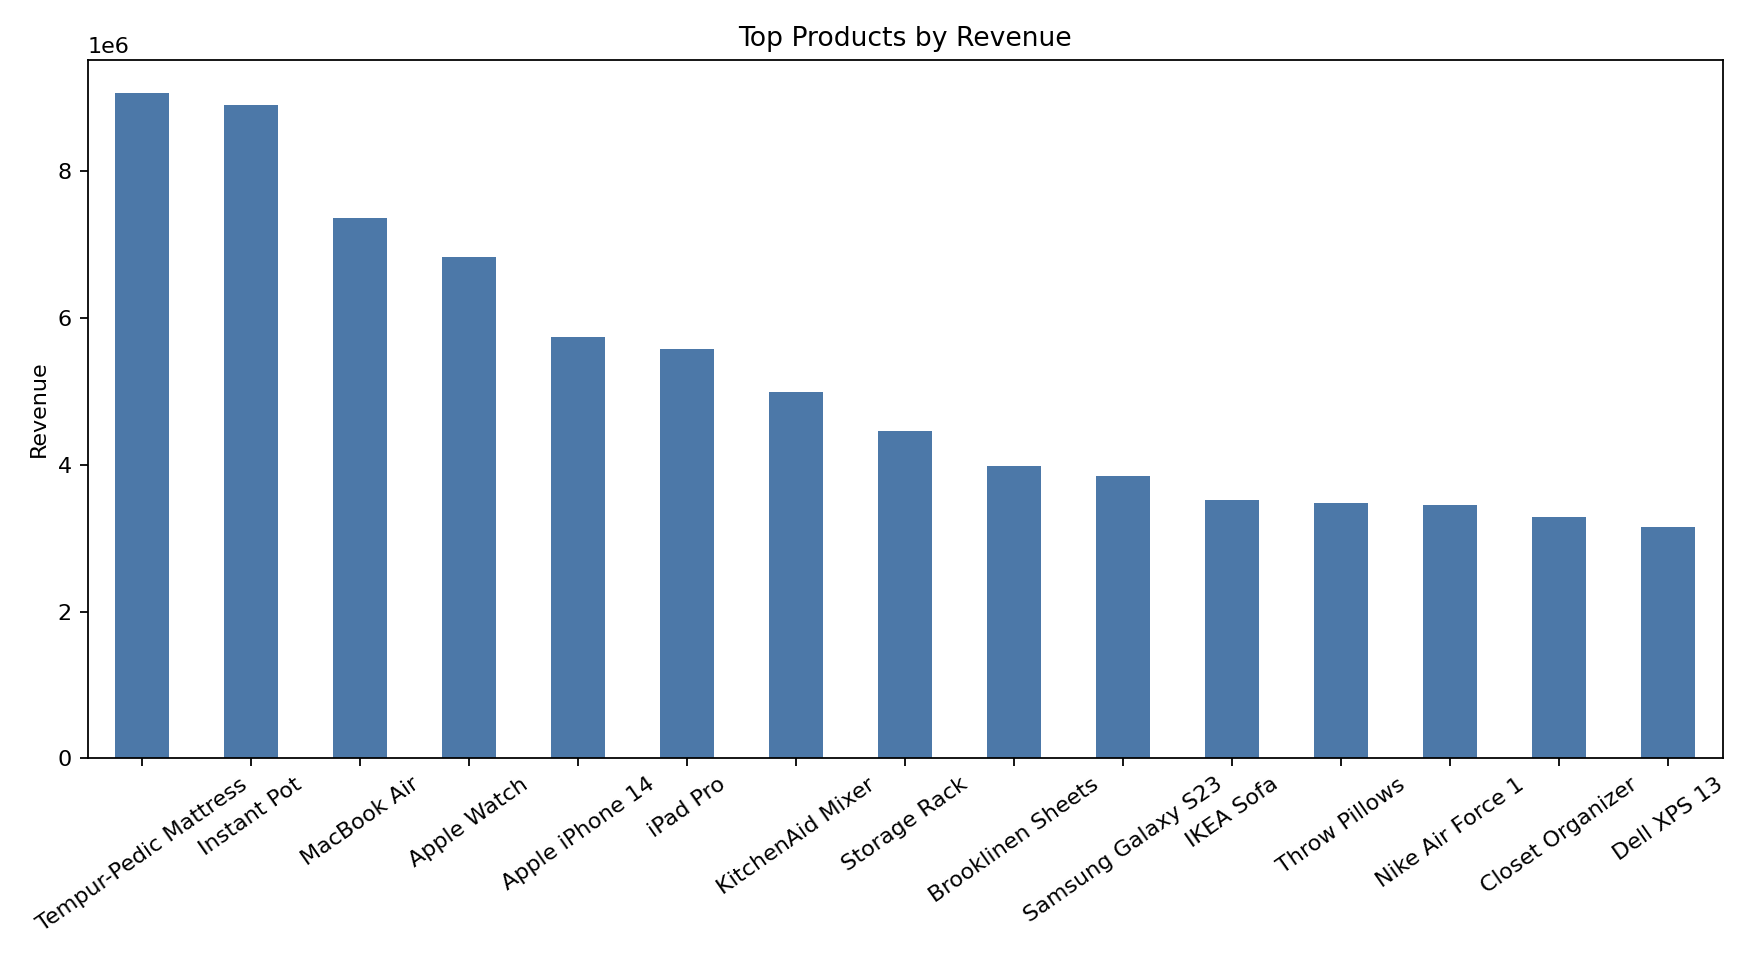
\includegraphics[width=\textwidth]{figures/lab02/top_products_by_revenue.png}
  \caption{Top products by revenue}
\end{figure}\
\vspace{4pt}
\begin{figure}[H]
  \centering
  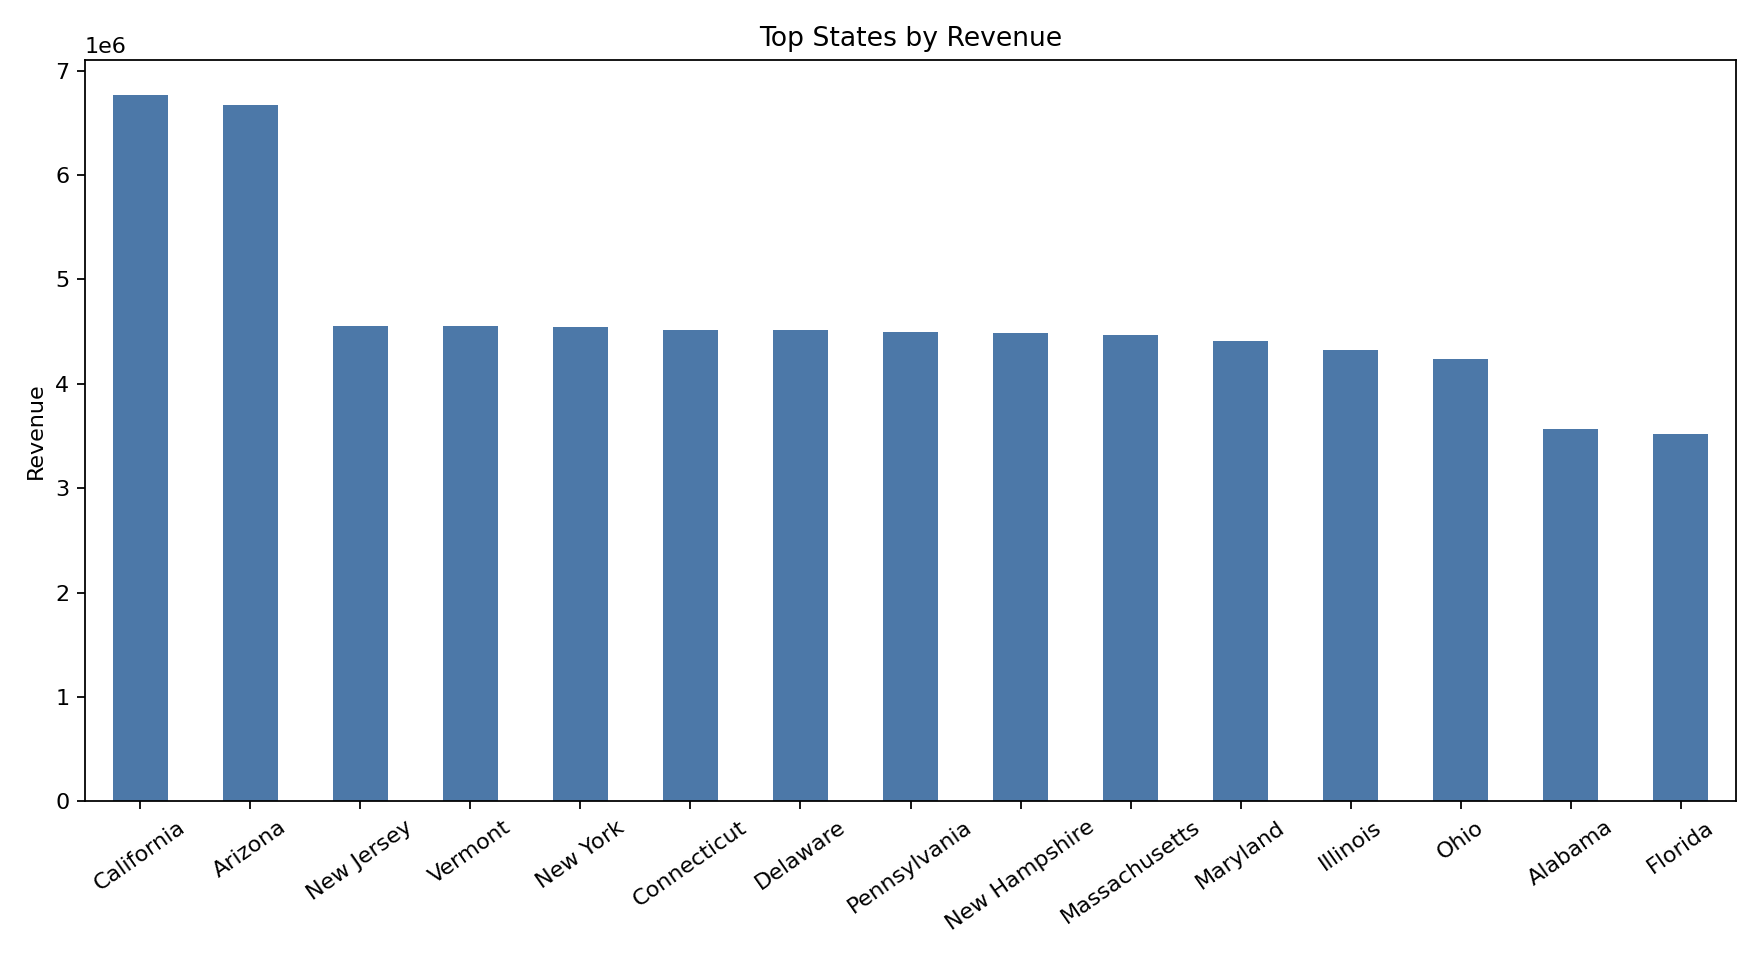
\includegraphics[width=0.48\textwidth]{figures/lab02/top_states_by_revenue.png}
  \caption{Top states by revenue}
\end{figure}
\end{figure}

\begin{notebox}
\textbf{HGB + Lag\_28 ensemble reduces RMSLE by 0.144 over the strong seasonal baseline.} The combination of boosting's non-linear pattern discovery with a seasonal baseline's stability is the key design pattern. Lag features consistently dominate feature importance — past sales are the strongest predictor of future sales. The 60/40 blend ratio balances pattern complexity against variance.
\end{notebox}
